\documentclass{thesis}
\newcommand{\normal}[2]{\mathcal{N}\left(\, {#1} \,,\,~{#2} \,\right)}
\newcommand{\multinormal}[4]{\mathcal{N}_{#1\times #2}\left(\, {#3} \,,\,~{#4} \,\right)}
\newcommand{\matrixnormal}[4]{\mathcal{MN}_{#1,#2}\left(\, {#3} \,,\,~{#4} \,\right)}

\newcommand{\vect}[1]{\boldsymbol{\mathbf{#1}}}
\newcommand{\mat}[1]{\boldsymbol{\mathbf{#1}}}

\newcommand{\tbm}[1]{$\mathbf{#1}$}
\newcommand{\tvect}[1]{$\boldsymbol{\mathbf{#1}}$}
\newcommand{\tmat}[1]{$\boldsymbol{\mathbf{#1}}$}

%\newcommand{\bm}[1]{\mathbf{#1}}
\newcommand{\paren}[1]{\left(#1\right)}

\newcommand{\texto}[1]{~~\text{#1}~~}

\newcommand{\til}[1]{\tilde{#1}}




\newcommand{\bfy}{\mathbf{y}}
\newcommand{\bfb}{\mathbf{b}}

\newcommand{\pinv}[1]{{#1}^{\dagger}}
\newcommand{\inv}[1]{{#1}^{-1}}
\newcommand{\trans}[1]{{#1}^\intercal}

\newcommand{\rmA}{\mathrm{A}}
\newcommand{\rmB}{\mathrm{B}}
\newcommand{\rmF}{\mathrm{F}}
\newcommand{\rmG}{\mathrm{G}}
\newcommand{\rmL}{\mathrm{L}}
\newcommand{\rmR}{\mathrm{R}}
\newcommand{\rmK}{\mathrm{K}}
\newcommand{\rmX}{\mathrm{X}}
\newcommand{\rmW}{\mathrm{W}}
\newcommand{\rmU}{\mathrm{U}}
\newcommand{\rmV}{\mathrm{V}}

\newcommand{\bfalpha}{\boldsymbol{\alpha}}
\newcommand{\bfbeta}{\boldsymbol{\beta}}


\newcommand{\calL}{\mathcal{L}}

\newcommand{\nullH}{\mathcal{H}_0}
\newcommand{\altH}{\mathcal{H}_1}

\begin{document}

\hyphenation{
cross-va-li-da-tion
}
%\titlehead{
    \parbox{1\textwidth}{\centering
   			\includegraphics[height=12mm]{Figures/logos.pdf}}%
    \vspace{12mm}}
\title{Genetic association of high-dimensional traits}
\subject{This dissertation is submitted for the degree of Doctor of Philosophy}
\author{Hannah Verena Meyer}
\date{September 2017}
\publishers{%
    %\vfill doesn’t work properly on title page due to excess glue
    \vspace{6\baselineskip}
  	University of Cambridge\\
  	Jesus College\\[0.2\baselineskip]
    European Bioinformatics Institute}

\lowertitleback{%
    \centering
    {\footnotesize The source code of the thesis is available at
        \url{https://github.com/HannahVMeyer/thesis}.}}


\maketitle


%This dissertation is the result of my own work and includes nothing which is the outcome of work done in collaboration except as declared in the Preface and specified in the text.

It is not substantially the same as any that I have submitted, or, is being concurrently submitted for a degree or diploma or other qualification at the University of Cambridge or any other University or similar institution except as declared in the Preface and specified in the text. I further state that no substantial part of my dissertation has already been submitted, or, is being concurrently submitted for any such degree, diploma or other qualification at the University of Cambridge or any other University or similar institution except as declared in the Preface and specified in the text. 

This dissertation does not exceed the limit of \num{60000} words as specified by the Biology Degree Committee.
% Introduction
\tableofcontents
%\listoffigures
%\listoftables

\chapter{GWAS of left ventricular wall thickness}
\label{chapter:GWAS-3Dheart}
The structure of the human heart is determined by an interplay of genetic factors and and complex environmental influences \citep{Payne1995, Sanoudou2005, OToole2008}. One common, heritable trait used to predict clinically relevant heart conditions is left ventricular mass (LVM). In particular, the increase in LVM is associated with an increased risk of heart failure and sudden death \citep{Haider1998,Post1997,Lorell2000}.  The increase in LVM through the thickening of the left ventricular wall is a direct response to a rise in hemodynamic burden which causes the hypertrophy of existing myocytes \citep{Lorell2000}. The thickening of the wall can occur in a symmetric fashion through concentric thickening of the ventricle with a small cavity dimension. However, about \num{58}\%  of all cases of left ventricular hypertrophy are asymmetric \citep{Davies1995} and the observed asymetry patterns are diverse in distribution and occurence \citep{Hughes2004,Florian2012}. A number of genetic factors have been shown to be involved in these asymmetric changes in the structure of the left ventricle \citep{Davies1995,Chen1999,VanderMerwe2008}. To date, genome-wide association studies (GWAS) in African American \citep{Fox2013}, Caucasian \citep{Vasan2007, Vasan2009, Arnett2009} and more recently Japanese cohorts \citep{Sano2016} have attempted to identify genomic loci that are significantly associated with LVM, where LVM was assessed using echocardiographic measures or 2D cardiac magnetic resonance (CMR) imaging. However, none of the studies find associations that pass the commonly applied genome-wide significance threshold. Many factors might have influenced the success of the studies and the lack of finding genetic associations such as lack in power through small sample or effect size. Given the genetic effects of the clinical LVM phenotypes observed \citep{Davies1995,Chen1999,VanderMerwe2008}, the assumptions for a genetic contribution to the natural variation in heart morphology holds, despite the negative results obtained in these studies. However, the asymmetric nature of changes in heart morphology might make LVM an inaccurate phenotype for detecting these genetic effects. To investigate genetic influences on overall heart structure instead of on a reduced representation such as LVM, spatially resolved, quantitative heart phenotypes are needed. 

A recent advance in CMR imaging is the use of 3D imaging of the heart as a whole as opposed to multiple transversal sections of the heart by 2D imaging. The latter technique has been the clinical gold standard but recent studies have shown that 3D imaging improves spatial resolution especially at the base and apex of the heart (\cref{fig:heart}) and can avoid technical issues arising from 2D imaging \citep{deMarvao2014}. Detailed images derived from the 3D imaging technique combined with genotype data would allow for an investigation into spatially-confined changes in heart morphology. Genetic association studies based on imaging phenotypes are widely applied In the field of neuroscience \citep{Filippini2009,Ho2010,Jahanshad2013,Hibar2015}. The first unbiased study using genome-wide genetic markers to find genetic associations with brain activity patterns was conducted by Stein and colleagues. They associated every voxel of 3D brain scans with all genetic markers. Following this approach, associating heart morphology as represented in the 3D scans would require testing approximately \num{140000} voxels. However, voxel-wise GWAS is limited in power and does not take into account any spatial correlation between the voxels \citep{Ge2014}. 

To overcome these limitations and offer more practical measurements for clinical use, De Marvao and colleagues have developed a technique to extract 3D features of the cardiac morphology from the 3D scans \citep{deMarvao2014}. As part of the `digital heart project' \citep{Cook2010}, they created the first at scale cohort of about \num{1500} detailed 3D statistical models of the variation in cardiac morphology from healthy volunteers. Based on these models, standard clinically relevant measurements such as LVM can be computed. Far beyond these simple 1D measurements, the 3D models allow spatially derived phenotypes such as left-ventricular wall thickness or curvature to be resolved for over \num{27000} coordinates. However, there still remains the substantial challenge in handling this still large number of correlated dimensions present in these models remain.

In the following chapter, I describe the genome-wide association study of phenotypes dervied from the 3D statistical models of the `digital heart project'. Within this project, I was responsible for the quality control and imputation of the genotypes, and conducted the GWAS from the 3D phenotypes. My colleagues collected the DNA samples, performed MRI scans and provided the 3D phenotyping. I will first describe the genotyping and phenotyping strategy and then show the results from applying different dimensionality reduction techniques to the 3D heart phenotypes. Based on the criteria described in \cref{chapter:DimReduction}, I chose the most suitable methods and conducted a GWAS with components derived thereof as proxy phenotypes. Finally, I investigated the significantly associated loci for any spatial association with the 3D heart phenotypes.

Using the genotype information which I processed and imputed, a preliminary publication on genetic associations was accepted for publication \citep{Biffi2017} and we are currently planning the publication of the analyses and results described in this chapter.



\section{Data}
\subsection{Genotypes}
\label{subsection:genotypes}
\paragraph{Quality Control.} Genotyping and genotype calling were carried out at the Genotyping and Microarray facility at the Wellcome Trust Sanger Institute, UK and Duke-NUS Medical School, Singapore. Genotypes were assessed in five batches using Illumina HumanOmniExpress- 12v1-1 (Sanger, two batches), Illumina HumanOmniEx\-press-24v1-0 (Duke-NUS, two batches) and Illumina HumanOmniExpress- 24v1-1 chips (Duke-NUS). \glspl{snp} were called via the GenCall software for clustering, calling and scoring of genotypes \citep{Teo2007}. For batches run on the same platform, genotype signals were combined and called in a single analysis, leading to three independent genotype batches: Sanger12 (\num{1344} samples), Duke-NUS12 (\num{284} samples), Duke-NUS3 (\num{96} samples). I carried out the \gls{qc} on the raw genotype calls, the phasing and the imputation, at a per-batch level. The final \gls{qc} of the imputed data was conducted across all batches and only \glspl{snp} passing the control in every batch were used in subsequent analyses. 

Prior to \gls{qc}, I matched the rsID descriptions (chromosome, chromosomal positions and allele order) of the three batches to the reference set I would use for imputation, a combined UK10K \citep{UK10KConsortium2015} and \num{1000} Genomes \citep{1000Genomes2015} reference panel. For rsIDs not included in the reference panel I retrieved location and allele order from the ensembl human variation annotation (GRCh37p13, 15.04.2016). rsIDs that matched to neither reference were removed from further analyses (\num{4681} across all chips). In order to avoid batch effects in \gls{snp} calling simply based on the probe sequences, I confirmed that probes targeting the same \gls{snp} on different chip versions had the same sequence. As this was the case, no \glspl{snp} were removed at this stage. 
I followed an adapted quality control protocol from \citet{Anderson2010} to asses the quality of the genotyping on a per-individual and per-marker level. Unless stated otherwise, the PLINK software (version 1.9) \citep{Purcell2007, Chang2015} was used for all \gls{qc} analyses. In summary, the per-individual \gls{qc} included the identification of individuals with discordant sex information, missing \gls{snp} rates (more than 3\% of \glspl{snp} not called) and heterozygosity rate outliers (three standard deviations outside of the mean heterozygosity rate). Population substructures arising due to different ethnical origins of samples were examined by comparing the sample genotypes to genotypes from the HapMap Phase III study \citep{HapMap2005} for four ethnic populations (with subpopulations, \cref{fig:kinshipQC} in the appendix). Samples that clustered with HapMap III individuals of Caucasian ancestry were kept for further analyses. The per-marker \gls{qc} included filtering of \glspl{snp} with missing call rate in more than \num{1}\% of the samples and \glspl{snp} which significantly deviate from Hardy-Weinberg equilibrium (HWE, \(p < 0.001\)). After removing samples and \glspl{snp} that failed \gls{qc}, I confirmed that any pattern of missing genotype information was not batch-specific. To analyse these patterns, I treated each pair-wise combination of batches as a case-control set-up and computed the differential missingness of \glspl{snp} common to all batches. None of the \num{631877} common \glspl{snp} had to be removed due to significant differential missingness (\(p < 10^{-5}\)). Table~\ref{tab:genoOverview} shows an overview of sample and \gls{snp} numbers before and after the \gls{qc} described above. The \gls{qc} plots for each step can be found in \cref{fig:sampleQC,fig:SNPQC,fig:kinshipQC} in the appendix. 
\\
% Table generated by Excel2LaTeX from sheet 'GenotypesSummary'
\begin{table}[htbp]
  \centering
  \caption[\textbf{Sample and SNP numbers before and after the QC. }]{\textbf{Sample and SNP numbers before and after the QC. } For each batch (first column), the number of male (m)/female (f) samples and \glspl{snp} before and after \gls{qc} are listed. Rate specifies the genotyping rate of samples within one batch after \gls{qc}. }
    \begin{tabular}{lrrrrrr}
    \toprule
          & \multicolumn{2}{c}{pre-\gls{qc}} &       & \multicolumn{3}{c}{post-\gls{qc}} \\
\cmidrule{2-3}\cmidrule{5-7}          & samples (m/f) & \glspl{snp}  &       & samples (m/f) & \glspl{snp}  & Rate \\
\cmidrule{2-7}    Sanger12 & \num{1344}  (\num{614}/\num{730}) & \num{719665} &       & \num{998} (\num{463}/\num{535}) & \num{677036} & \num{0.998} \\
    Duke-NUS12 & \num{284} (\num{118}/\num{166}) & \num{716503} &       & \num{179} (\num{68}/\num{111}) & \num{682016} & \num{0.998} \\
    Duke-NUS3 & \num{96} (\num{48}/\num{48}) & \num{7713014} &       & \num{62} (\num{34}/\num{28}) & \num{657497} & \num{0.998} \\
    \bottomrule
    \end{tabular}%
    \label{tab:genoOverview}%
\end{table}%

\paragraph{Phasing and imputation.} Phasing and imputation were conducted in two separate steps. For phasing, I used SHAPEIT ( version 2.r727) \citep{Delaneau2012,Delaneau2013} to generate estimated haplotypes for each sample that passed the quality control. The window size for phasing was set to 2Mb, and the number of conditioning states per \gls{snp} to \num{200}. All other parameters were set to default values. The phased genotypes were then imputed with IMPUTE2  (version 2.3.0) \citep{Marchini2007, Howie2009} based on the combined \num{1000} Genomes \citep{1000Genomes2015} and UK10K \citep{UK10KConsortium2015} reference panel. I set the imputation interval to 3Mb,  with a buffer region of \num{250}kb on either side of the analysis interval. As suggested in the user manual, I used an effective population size of \num{20000} and set the number of reference haplotypes to use to \num{1000}. Again, for the additional, non-specified parameters the default was used.

\paragraph{Combining datasets.} I combined the three genotype batches after imputation and filtered them again on a per-sample and per-marker level. On the per-sample level, I excluded related individuals because of the difficulties that might arise in adjusting for relatedness in the processing of the phenotypes via dimensionality reduction. A more detailed explanation will follow in \cref{section:DimRed-heart}. Relatedness was estimated by the proportion of \glspl{snp} shared between two individuals and subsequent calculation of identity by descent estimated as PI\_HAT on the genotyped \glspl{snp} via PLINK as described by \citep{Anderson2010}. For any pair of individuals with a PI\_HAT of greater than \num{0.125}, the individual with the higher \gls{snp} calling rate was retained in the analysis. For the quality control on the per-marker level, I used the statistical information about the imputation certainty, the `info' metric,  given as additional output by IMPUTE2. The metric typically takes values between zero and one, with values closer to one indicating high imputation certainty. I excluded any \gls{snp} with an info score of less than \num{0.4} in at least one of the batches. Approximately \num{60}\% of all imputed \glspl{snp} were excluded based on this criterion.  After combining the datasets, I used SNPTEST (v2.5) \citep{Marchini2010} to compute the \gls{maf} and p-value for deviation from Hardy-Weinberg equilibrium per \gls{snp}. \glspl{snp} with a significant deviation from Hardy-Weinberg equilibrium (\(p <0.001\)) and a minor allele count of less than \num{20} alleles (corresponding to a minor allele frequency of \num{0.008}) were removed, leading to a decrease in \glspl{snp} of another approximately \num{41}\%, a total reduction from imputed \glspl{snp} to \glspl{snp} that passed every filtering criteria of \num{23}\%.  A summary showing the magnitude of the number of imputed \glspl{snp} per batch, the number of \glspl{snp} after imputation quality filtering and filtering for \gls{maf} and Hardy-Weinberg-equilibrium deviation is depicted \cref{fig:imputeQC}. Exact numbers can be found in \cref{tab:imputationQC}.

\begin{figure}[hbtp]
	\centering
	\includegraphics[trim = 0mm 0mm 0mm 20mm, clip, width=\textwidth]{Chapter5/Figures/combinedSNPsperChr.pdf}
	\caption[\textbf{Overview of SNP numbers after imputation and imputation quality control. }]{\textbf{Overview of SNP numbers after imputation and imputation quality control. } The imputation of the \glspl{snp} based on the genotypes from \gls{snp} arrays was done on a per-batch level. The number of \glspl{snp} for each batch after imputation is shown as red bars and is very similar for each of the three batches (exact numbers in \cref{tab:imputationQC}). About \num{40}\% of \glspl{snp} are retained after filtering for the `info` metric (light grey bars). The bars in dark grey show the final number of \glspl{snp} per chromosome. }
 	\label{fig:imputeQC}
\end{figure}
%
After imputation and imputation quality control, the dataset contains \num{9233118} \glspl{snp} from \num{1207} samples. IMPUTE2 yields imputed genotypes encoded in triplets of posterior probabilities for the possible allele combinations \((AA, AB, BB)\). These probabilities were converted into expected genotypes \(G\) by the dosage model \citep{Howie2011}:

\begin{equation}
	G = 0 \times p(AA) + 1 \times p(AB) + 2 \times p(BB) = p(AB) + 2 \times p(BB)
\end{equation}


\subsection{Phenotypes}
\label{subsection:phentoypes}
The phenotyping was done by my collaborators, in particular Antonio de Marvao. CMR imaging and generation of 3D models of the left ventricle derived from these images were conducted at Hammersmith Hospital, London. In the following, I will briefly describe the methodology of their automatic phenotyping approach. The technical details of the image acquisition, the analysis and their improved performance over standard methods are described in detail in \citep{deMarvao2014}. 

In the automated phenotyping approach developed by Antonio de Marvao and colleagues, cardiac structures are accurately extracted from raw 3D cadiac magnetic resonance images (\cref{fig:segmentation}, \subfig{1}) to generate 3D models of the individuals' hearts  (\cref{fig:segmentation}, \subfig{3}). The cardiac structures of interest in this study were left ventricular cavity, myocardium and right ventricular bloodpool at end-diastole and end-systole. The approach uses a local database of segmented and quality controlled cardiac \gls{mri} atlases, to which each newly acquired image is compared. The database was created by Antonio, who initially selected \num{20} subjects and manually classified the approximately \num{140000} voxels per image into the three categories named above. In the database generation phase, subsequent successful segmentation of new images described by the method below were added, yielding a total of \num{1072} images in the final database. In addition to serving as a database for the segmentation algorithm, the database images were used to generate a template image of average heart size, position and orientation. 

For each new image, six landmarks are manually placed on the image, which enables the subsequent image registration between the target and the atlas images. After registration, a multi-atlas PatchMatch algorithm finds corresponding patches of adjacent voxels within the atlas and target images (\cref{fig:segmentation},\subfig{2}). Each patch in the target image is given the label of the closest matching atlas patches and combining the labels of all patches produces the final segmentation. Lastly, the segmented image is registered to the template image to make the spatial coordinates in the 3D models consistent between all samples.  

Using a surface rendering algorithm allows for the extraction of information from a segmentation volume such as the left ventricular myocardium into a surface representation. Through such an algorithm, the wall thickness, curvature and  fractional wall thickening at \num{27623} positions in the left ventricle were extracted for each individual (\cref{fig:segmentation}\subfig{2}). %In addition, the left ventricular mass was computed based on the volume and density of the myocard. 
\\

\begin{figure}[h]
	\centering
	\includegraphics[trim = 0mm 0mm 0mm 0mm, clip,width=\textwidth]{Chapter5/Figures/Segmentation.pdf}
	\caption[\textbf{Cardiac phenotyping based on cardiac magnetic resonance images. }]{\textbf{Cardiac phenotyping based on cardiac magnetic resonance images. }1. Detailed 3D images of the heart were acquired in the left ventricular short axis plane from base to apex. 2. The images were segmented into left ventricular myocardium (green), left ventricular blood pool (red) and right ventricular blood pool (yellow) and registered to a common template image via a multi atlas-based technique. 3. Through a surface rendering algorithm of the registered segmentation, a 3D model of the heart was generated and wall thickness measurements derived at \num{27623} positions of the left ventricle. The left ventricle is shown in solid colors, with the color scheme representing average wall thickness, increasing from light to darker colors. As a point of reference, the right ventricle is depicted as a mesh.}
 	\label{fig:segmentation}
\end{figure}
%
To assess the reproducibility of the phenotyping approach, one individual was scanned eight times and the images segmented as described above. These repeat scans allowed for the quantification of variation in the segmentation by the \gls{cv}. The \gls{cv} is a standardised measure of dispersion and is defined as the ratio of the standard deviation to the mean value. I computed the \gls{cv} for each of the \num{27623} positions in the 3D heart model across the eight scans and projected the results onto the template image (\cref{fig:reproducibility}). Overall, the dispersion is very low i.e. the reproducibility high. Only at the base of the left ventricle in proximity to the right ventricle can a slight increase in dispersion be observed (\cref{fig:reproducibility}, red area). The low dispersion shows the accuracy of the segmentation and surface rendering methods. Based on this result and further quality control criteria such as the comparison between the segmentations and manually labelled images (details in \citep{deMarvao2014} the wall thickness measurements were considered reliable phenotypes for subsequent analyses. 
\\ 

\begin{figure}[h]
	\centering
	\includegraphics[trim = 0mm 0mm 0mm 0mm, clip,width=0.5\textwidth]{Chapter5/Figures/Dispersion.pdf}
	\caption[\textbf{Phenotype reproducibility. }]{\textbf{Phenotype reproducibility. }The dispersion in left ventricular wall thickness at \num{27623} positions was computed as the standard deviation over the mean across eight segmentation derived from independent scans of one individual. The right ventricle is shown as a point of reference (mesh structure). }
 	\label{fig:reproducibility}
\end{figure}
%

%\bibliography{myLibrary2}
%\bibliographystyle{ebi}

%\beginsupplement
%\section{Quality control: genotyping}

\begin{figure}[hbtp]
	\centering
	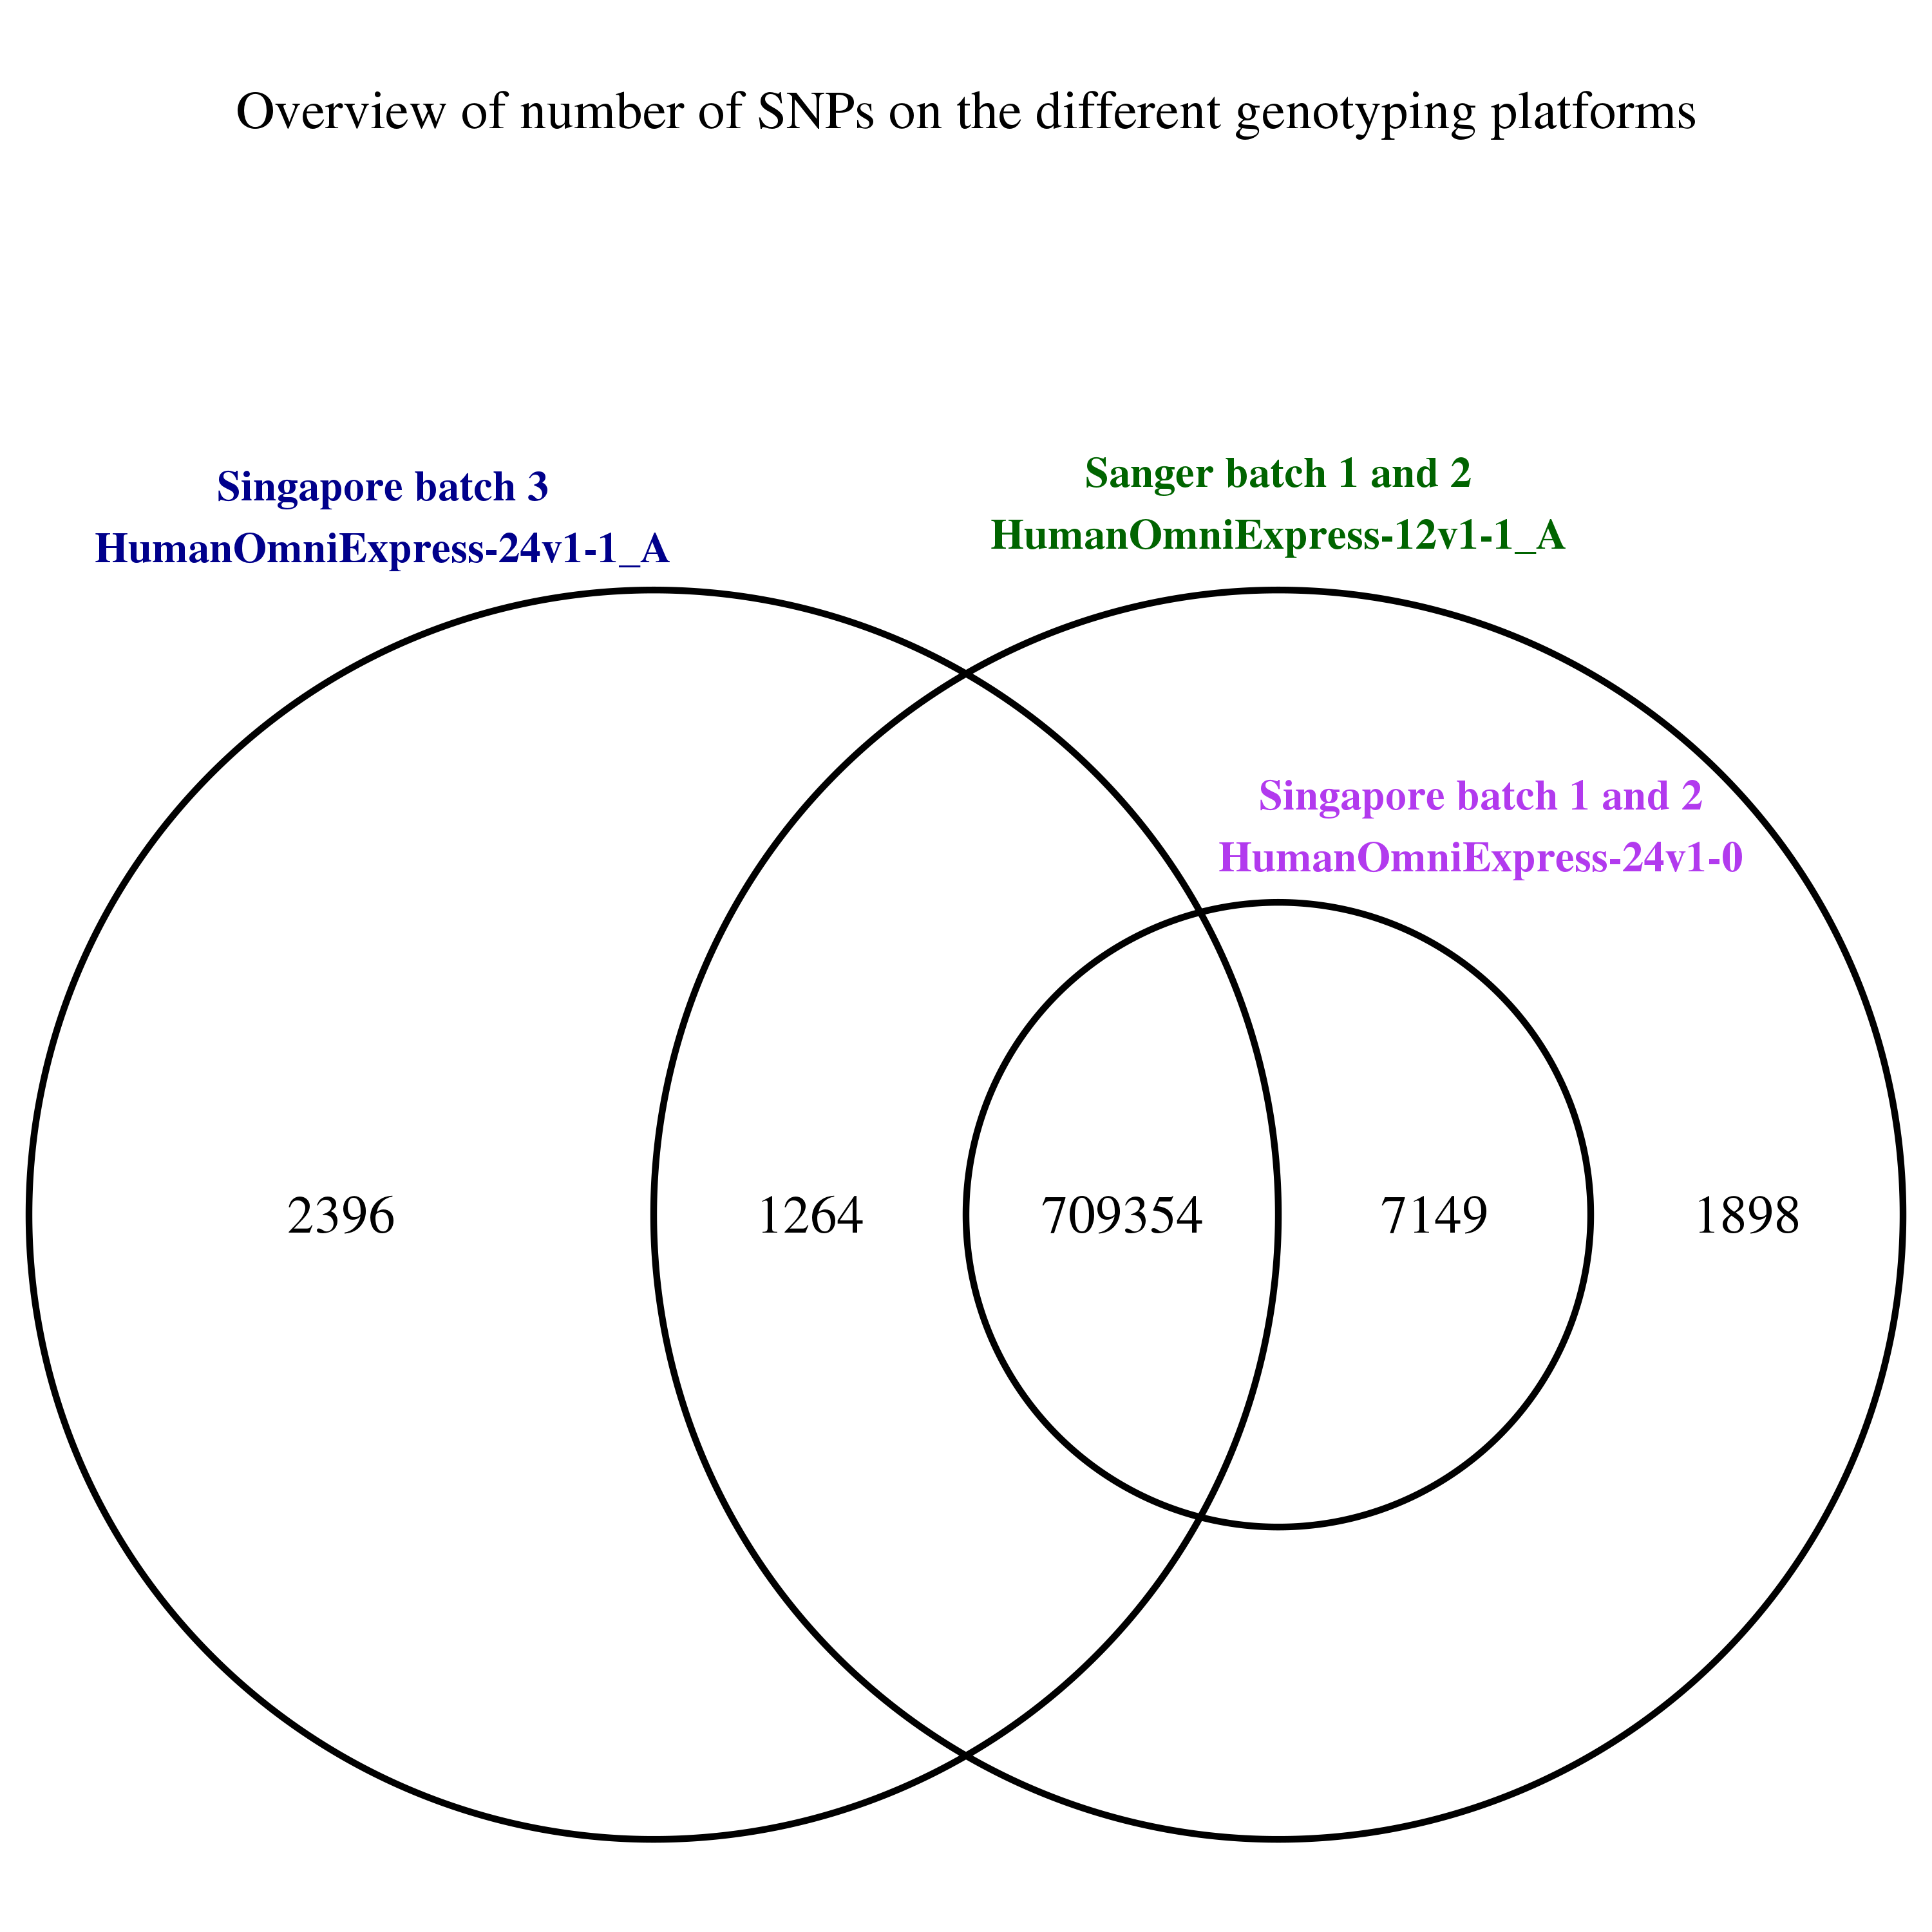
\includegraphics[trim = 0mm 0mm 0mm 20mm, clip, width=0.8\textwidth]{Figures/Venn_genotyping_batches.png}
	\caption{\textbf{.} .}
 	\label{fig:probeoverlap}
\end{figure}

\begin{figure}[hbtp]
	\centering
	\includegraphics[trim = 0mm 0mm 0mm 20mm, clip, width=0.8\textwidth]{Figures/SampleQC.pdf}
	\caption{\textbf{.} .}
 	\label{fig:sampleQC}
\end{figure}

\begin{figure}[hbtp]
	\centering
	\includegraphics[trim = 0mm 0mm 0mm 20mm, clip, width=0.8\textwidth]{Figures/SNPQC.pdf}
	\caption{\textbf{.} .}
 	\label{fig:SNPQC}
\end{figure}

\begin{figure}[hbtp]
	\centering
	\includegraphics[trim = 0mm 0mm 0mm 20mm, clip, width=0.8\textwidth]{Figures/kinshipQC.pdf}
	\caption{\textbf{.} .}
 	\label{fig:kinshipQC}
\end{figure}

\section{Quality control: imputation}

\begin{figure}[hbtp]
	\centering
	\includegraphics[trim = 0mm 0mm 0mm 20mm, clip, width=0.8\textwidth]{Figures/perBatchSNPsperChr.pdf}
	\caption{\textbf{.} .}
 	\label{fig:imputeQC}
\end{figure}
\end{document}


\clearpage
\chapter*{Summary}
\addcontentsline{toc}{chapter}{Summary}
\label{section:summary}

\begin{singlespace}
Over the past ten years, more than \num{4000} genome-wide association studies (GWAS) have helped to shed light on the genetic architecture of complex traits and diseases. In recent years, phenotyping of the samples has often gone beyond single traits and it has become common to record multi- to high-dimensional phenotypes for individuals. Whilst these rich datasets offer the potential to analyse complex trait structures and pleiotropic effects at a genome-wide level, novel analytic challenges arise. This thesis summarises my research into genetic associations for high-dimensional phenotype data.

First, I developed a novel and computationally efficient approach for multivariate analysis of high-dimensional phenotypes based on linear mixed models, combined with bootstrapping (LiMMBo). Both in simulation studies and on real data, I demonstrate the statistical validity of LiMMBo and that it can scale to hundreds of phenotypes. I show the gain in power of multivariate analyses for high-dimensional phenotypes compared to univariate approaches, and illustrate that LiMMBo allows for detecting pleiotropy in a large number of phenotypic traits.

Aside from their computational challenges in GWAS, the true dimensionality of very high-dimensional phenotypes is often unknown and lies hidden in high-dimensional space. Retaining maximum power for association studies of such phenotype data relies on using an appropriate phenotype representation. I systematically analysed twelve unsupervised dimensionality reduction methods based on their performance in finding a robust phenotype representation in simulated data of different structure and size. I propose a stability criteria for choosing low-dimensional phenotype representations and demonstrate that stable phenotypes can recover genetic associations.

Finally, I analysed genetic variants for associations to high-dimensional cardiac phenotypes based on MRI data from \num{1500} healthy individuals. I used an unsupervised approach to extract a low-dimensional representation of cardiac wall thickness and conducted a GWAS on this representation. In addition, I investigated genetic associations to a trabeculation phenotype generated from a supervised feature extraction approach on the cardiac MRI data.

In summary, this thesis highlights and overcomes some of the challenges in performing genetic association studies on high-dimensional phenotypes. It describes new approaches for phenotype processing, and genotype to phenotype mapping for high-dimensional datasets, as well as providing new insights in the genetic structure of cardiac morphology in humans.


\end{singlespace}


% Increasing sample sizes have allowed to extend the genotype to phenotype mapping from common to rare variants.
% far beyond standard methods that work in the regime of up to 30 phenotypes. 

\chapter{Introduction}

The field of quantitative genetics has come far since Fisher's initial studies on growth traits in wheat in 1918 \citep{}. While back then the concept of inheritance existed, little was known about the molecule responsible.  The discovery of the DNA structure by Franklin, Watson and Crick and technical break-throughs in analysing its sequence some xx years later, have allowed to investigate genetic variance on a much more detailed scale, moving from whole chromosomes and linkage studies to the analysis of DNA variation on a single-base pair level. The developments gentoyping and sequencing technologies in the recent years, have made large scale studies on genetic variation feasible. With the sinking costs of genotyping techniques, the number of samples investigated has risen and studies investigating effect of single DNA bases often comprise thousands of individuals, especially in the field of human genetics.  Together with the increased number of samples available in these studies, the number of phenotypes that are measured for each individual has grown from a few measurements to tens or even hundreds. The availability of these rich datasets provides great opportunities in studying genetic variations and its outcomes, such as studying pleiotropy and xx.  However, it also poses technical challenges in analysing these dataset. 

 Many cohort studies now have rich, high dimensional datasets ranging from studies in model organism such as yeast and arabidopsis thaliana to human molecular, morphological or imaging derived traits \citep{Bloom2013,Atwell2010,Astle2009,Shaffer2016,Stein2010}. However, these cohorts have often been analysed trait by trait partly for simplicity and partly because of a paucity of models suitable for the anlaysis of the high dimensional phenotype data.

\section{Multi-trait mapping}
Many cohort studies today, ranging from studies in model organism such as yeast and arabidopsis thaliana to human, have rich, high dimensional datasets including molecular, morphological or imaging derived traits \citep{Bloom2013,Atwell2010,Astle2009,Shaffer2016,Stein2010}. However, these traits have often been analysed separately,  partly for simplicity and partly because of a paucity of models suitable for the anlaysis of high-dimensional phenotype data. A variety of multi-trait models have been developed which can be broadly grouped into three different classes: i) dimensionality reduction techniques, ii) meta-analysis approaches and iii) multivariate regression models (reviewed in \citep{Shriner2012,Yang2012}). 
\paragraph{Dimensionality reduction techniques}  
Dimensionality reduction methods in genotype-phenotype mapping seek to find a linear combination of the phenotypes \(\mat{Y} \in \mathcal{R}^{N,P}\) into a lower dimensional space \(\tilde{\mat{Y}} \in \mathcal{R}^{N,K}\):
\begin{equation}
\tilde{\mat{Y}} = b_1\mat{y}_1 + b_2\mat{y}_2 + \dots + b_P\mat{y}_P
\end{equation}

Two commonly employed dimensionality reduction methods are principal component analysis (PCA) and canonical correlation analyses (CCA). In PCA, the components of the new phenotype representation are called principal components (PC) and are the eigenvectors \tmat{W} of the empirical covariance matrix \(\mat{Y}^T\mat{Y}\): \(\mat{Y}^T\mat{Y} = \mat{W}\mat{\Lambda}\mat{W}^T\). The eigenvalues \(\Lambda\) corresponding to the PCs are equivalent to the variance explained by their components. The transformation of the phenotype data into principal components leads to a projection where the highest amount of phenotypic variance explained lies in the first component, the second highest variance in the second component and so forth. The dimensionality reduction is achieved by using the first \(K\) principal components until the cumulative sum of the eigenvalues reaches a predefined threshold of total phenotypic variance that should be retained. These \(K\) principal components are used as proxy phenotypes for the association study. PCA as a dimensionality reduction technique has for instance been used in studies to find links between genotypes and facial features or obesity phenotypes \citep{Liu2012,Claes2014,He2008}. Recently, Aschard and colleagues \ref{Aschard2014} demonstrated that simply focusing on the principal components with the highest variance might not exploit the full potential of using PCA for genetic association. They propose a model of combined PCA where the PCs are grouped based on the level of variance they explain. They show a power gain in detecting genetic associations compared to simple approaches of only testing the top few PCs.

While the PCA dimensionality reduction approach focus on the phenotype space and subsequent association with the genotypes, CCA finds the optimal transformation of \tmat{Y} into \(\tilde{\mat{Y}}\) while simultaneously testing for the association with the genotypes. Originally proposed by Hotelling for any set of variables that remain invariant under internal linear transformation\citeyear{Hotelling1936}, in quantitative genetics CCA seeks to maximise the canonical correlation \(\hat{\rho}\) between  \(\tilde{\mat{Y}}= A^T\mat{Y}\) and a genotype \(\mat{X} \in \mathcal{R}^{N,1}\):   \(\hat{\rho} = cor(\mat{X},\tilde{\mat{Y}}) = \Sigma_{XY}A(A^T\Sigma_{YY}A\Sigma_{XX})^{-\frac{1}{2}}\). \(\Sigma_{YY},\Sigma_{XX} \text{ and } \Sigma_{XY}\) are the empirical sample covariance matrices of the phenotypes, the genotypes and cross-covariance of the phenotypes and genotypes, respectively. \(\hat{\rho}\) is maximised by finding the squared root of the largest eigenvalue of the \(\Sigma_{YY}^{-1}\Sigma_{YX}\Sigma_{XX}^{-1}\Sigma_{XY}\) covariance matrix and the corresponding eigenvector \tmat{A} contains the coefficients for constructing \(\tilde{\mat{Y}}\) \citep{Yang2102}. CCA finds the transformation \(\tilde{\mat{Y}}\) that explains the maximum amount of the covariation between the genotype and all traits. The significance of the correlation i.e. the genotype-phenotype association can be tested via Bartlett's likelihood ratio test with the null hypothesis of \(\text{H}_\text{0: }\Sigma_{YX} = 0\) \citep{Bartlett1941}. Ferreira and Purcell showed in simulations that CCA with multiple traits and one genetic marker \tmat{X} controls well for type I errors and has increased power compared to multivariate tests. In order to extend the CCA method to more than one marker, the genotypes also undergo a linear transformation: 
 \(\hat{\rho} = cor(B^T\mat{X},A^T\mat{Y}) = B^T\Sigma_{XY}A(A^T\Sigma_{YY}AB^T\Sigma_{XX}B)^{-\frac{1}{2}}\) and the maximum \(\hat{\rho}\) is found by solving for the largest eigenvalue of both \tmat{A} and \tmat{B}. As the number of genotype markers in GWAS exceeds the number of samples, estimates of the covariance matrix \(X^TX\) become unreliable \citep{Schaefer2005}. Several methods have been developed to circumvent this issue, making use of sparse matrices \citep{Parkhomenko2009} or a priori grouping of the genotypes \citep{Naylor2010}. 

 \paragraph{Meta-analysis approaches}
Meta-analysis approaches combine the simplicity of the univariate approaches with the advantages of the multivariate approach. For each phenotype, a univariate association study is conducted and the summary stastics of these tests combined. Many methods for combining the summary statistics \citep{Xu2003,Yang2010,Yang2012,Bolormaa2014} go back to the work by O'Brien \citep{O'Brien1984}, who proposed to use a linear combination of the observed test statistics for each univariate test \(\mat{T} =(T_1, \dots, T_P)^T\) as the new statistics to be evaluated for significance.  \tmat{T} is asymptoctically normal distributed with mean \(\mat{\mu} = (\mu_1,\ldots, \mu_P)^T\) and covariance matrix \(\mat{\Sigma}\). O'Brien stastistic allows for testing the Null hypothesis \(H_0: \mu = 0\) against the alternative hypothesis of  \(H_1: \mu_p \ge 0, p=1, \ldots , P \) and is most powerful if \(\mu_1= \ldots =\mu_P\) \citep{Xu2003}. It is defined as: \(S = \mat{J}^T \mat{\Sigma}\mat{T}\), with \(\mat{J} = (1, 1, \ldots, 1)^T\).  The statistic has been modified in a number of studies, by adapting either the weighting matrix \tmat{J}, the covariance matrix \tmat{\Sigma} or both. Xu and colleagues \citeyear{Xu2003} optimised \(S\) to allow for testing against a general \(\mu\) rather then for a case where  \(\mu_1= \ldots =\mu_P\) by allowing for flexible, but restrained weights in \tmat{J}. Similarily, Yang and colleagues  \citeyear{Yang2010} proposed non-uniform weights to reflect heterogeneity in the means and use a sample splitting and cross-validation approach to determine the optimal weights. 
While the previous two studies showed an increase in power for using the combined statistic, they either used a small marker set or small number of phenotypic traits.  Bolormaa and colleagues showed that these power gains also hold for genotype to phenotype mapping of 32 traits across all genome-wide markers \citep{Bolormaa2014}. In their study, the weights of O'Briens proposal are substituted by the signed t-statistic. 

\paragraph{Regression models} There are a number of different regression models that allow for the multivariate analysis of phenotypes. Among them are graphical models, generalized estimation equations and frailty models, for which a summary of methods and application can be found in \citep{Shriner2012,Yang2012}. Here, I will focus on describing the development of multivariate linear regression models for genotype-phenotype mapping. The underlying models and their derivation have been described in \cref{sec:intro}. Before the era of GWAS, QTL mapping in linkage experiments have demonstrated the increase in power when jointly analysing traits with common underlying genetics. Jiang and colleagues \citeyearpar{Jiang1995} proposed a multi-trait model where the phenotypes are jointly modeled as the sum of the fixed genetic effects of interest, fixed effects for genetic background variation and residual noise. They show that the joint analysis of traits can increase power to detect the underlying genetics and can increase the precision of the parameter estimates. The significance of the association is determined via a likelihood ratio test of the parameter estimates under the Null model where the fixed genetic effect is zero and the parameter estimates under the alternative model. The alternative model design depends on the underlying biological hypothesis regarding the effect of the genetic variant. Here, Jiang and colleagues differentiate hyptheses for a simple joint mapping of phenotypes, pleiotrophy and gene-environment interactions. Joint mapping does not make any assumptions about the underlying genetic architecture and simply tests if an association can be found when both traits are analysed jointly, i.e. the effect of the genetic variant is non-zero for at least one of the traits. This hypothesis can be extended in requiring that the effect on both traits is unequal to zero. In this case, the genetic variant is considered to be pleiotrophic. To test for gene-environment interaction, the different conditions a trait was studied in can be treated as different traits and be jointly mapped. If the effect size estimates of the genetic variant are not equal, the variant is considered to have environmental interactions.  Methods developed thereafter often use the same underlying hypotheses for the mapping, but different techniques for the evaluation of the significance. For instance, two other groups developed methods for the joint analysis of traits based specifically on the residual sum of squares (RSS) matrix of the standard linear model (\cref{eq:lm}) estimated at each locus tested \citep{Knott2000,Korol2001}. In the model proposed by Knott and Haley, the different properties and descriptors of the RSS are used to determine the significance of the QTL mapping. To test for pleiotropy for instance, the determinent of the RSS at the test locus is compared to the RSS of the null model of no association. In contrast, Korol and colleagues propose to use the RSS of the multi-trait mapping as a means for trait transformation and dimensionality reduction. The resulting one-dimensional trait per sample is fitted in a single-trait test for significance testing.  While methods described so far have only used fixed genetic effects, Korte and colleagues \citeyear{Korte2012} were the first to introduce a random genetic effect into the model. Based on the original model by Jiang, they substituted the fixed effect accounting for background genetics by a random effect, turning the multivariate linear model into a mulitvariate linear mixed model (Equation~\ref{eq:lmm}). Based on these principals and method development for the efficient analysis of large cohort sizes, a number of publically available frameworks for the genome-wide mapping of a moderate number of traits via multivariate linear mixed models were developed. \citep{Korte2012,Yang2011,Lippert2014,Zhou2014,Casale2015}. 

Out of the differerent approaches described above, multivariate linear mixed models (LMMs) have the additional advantage that they can control for population structure (\cref{sec:intro}). In LMMs, both the residual noise and the genetic backgound are modeled as random effects. For the random genetic effect, a complex covariance structure can be modeled such that family structure and relatedness captured in the genotypes can be exploited to model background genetic correlations in phenotype\citep{Yu2006,Kang2008} (\cref{eq:lmm}). The random effects are assumed to be composed of a sample-to-sample and trait-to-trait covariance component. The genetic sample covariance can be obtained from the data itself, e.g. using a genetic relationship matrix (GRM) or identity by descent, whereas the trait covariance terms need to be estimated from the observed data. Since the introduction of LMM for multi-trait GWAS studies, LMMs have been extended to handle the large sample sizes obtained in particular in human studies, allowing for cohort sizes of \red{xxx}  individuals \citep{Zhou2014}. However nearly all current methods scale poorly in the number of traits ($P$) due to a bottle neck caused by estimating the trait covariance terms. 

Together with Francesco Paolo Casale, a PhD student in Oliver Stegle's research group at the EBI, I developed a simple, but surprisingly effective heuristic which uses a linear mixed model with bootstrapping (LiMMBo) that allows for the analysis of datasets with a large number of phenotypic traits. In order to validate LiMMBo and show its applicability to high-dimensional phenotypes, I developed a phenotype simulation framework which allows for the simulation of well-defined phenotypes with different underlying genetic structures and noise distributions. This chapter describes this simulation strategy and the LiMMBo approach and its validity. 

\section{Genetic variation}
\section{Genome-wide association studies}
\begin{figure}[hbtp]
	\centering
	\includegraphics[trim = 0mm 0mm 0mm 0mm, clip, width=\textwidth]{Introduction/Figures/GenotypePhenotype.pdf}
	\caption[\textbf{.}]{\textbf{.} } 
	 	\label{fig:GenoPheno}
\end{figure}

\subsection{From genotype arrays to genome-wide SNP data}
\begin{itemize}
	\item Reference panel: HapMap, 1000Genomes, Uk10K
	\item Phasing and Imputation
\end{itemize}

\subsection{From molecular to organismal phenotypes}
\begin{itemize}
	\item eQTLs, eWAS
	\item intermediate phenotypes: organ level, brain, facial morpholgy
	\item case-control studies
\end{itemize}

\subsection{Linear Mixed Models}

Fixed genetic background componts are standardly modeled via principal components (PCs) of genotype data \citep{Price2006} and have been shown to adjust well for population structure based on ancestry differences \citep{Patterson2006}. However, PCs perform poorly in modeling family structure or cryptic relatedness.  By modeling genetic background as a random effect, more complex covariance structures can be used such that correlations in phenotype reflect family structure and relatedness \citep{Yu2006,Kang2008}.
	
Pruning for LD structure to construct kinship matrices \citep{Eu-ahsunthornwattana2014}
Derivation of kinship matrix as  \(\frac{1}{7}\) \citep{Speed2012}
	
\subsection{Linear models}
In genotype to phenotype mapping, the most simple linear model (LM) describes the linear relationship between a phenotype \(y\) and a genetic marker \(x\). Optionally, known covariates \(F\) can be included as explanatory variables. There are a variety of different types of models, depending on the structure of background effects and the number of phenotypes that are modeled simultaneously. In the following, a short description of the models relevant for this project is outlined. 

\label{sec:ssection:lm}
\paragraph{Uni-variate linear models for genetic analyses}
The uni-variate LM models a single phenotype \(y\) as the sum of a fixed effect of the genetic marker \(x\) and \(K\) known covariates \(F\) and residual noise \(\psi\) across \(N\) samples:

\begin{equation}
\mat{y} = \mat{F}\mat{\alpha} + \mat{x}mat{\beta} + \mat{\psi},\text{ }
\mat{\psi} \sim \normal 0 {\sigma_e^2\matsub{I}{N}}.
\label{eq:lm-uv}
\end{equation}

with
\begin{align*} 
& \text{the phenotype vector } \mat{y} \inR N 1,\\
& \text{the matrix of $K$ covariates }\mat{F} \inR N K,\\
& \text{the effect of covariates } \mat{\alpha} \inR K 1,\\
& \text{the genetic profile of the SNP being tested }\mat{x} \inR N 1 \text{and}\\
& \text{the effect size of the SNP } \mat{\beta} \inR x x \\
\end{align*} 


\noindent The association between phenotypes and the genetic markers can be assesed by testing the hypothesis that the genetic variant has an effect \(\beta \neq 0\) versus having no effect on the phenotype. The log likelihood ratio (LLR) test statistic \(\Lambda\) is a commonly used statistic to compare the likelihood of the full model \taltH (Equation~\ref{eq:lm-uv}) with \(\beta \neq 0\) to the one of the Null model \tnullH:
\begin{equation}
\nullH: \mat{y} =\mat{F}\mat{\alpha}  + \mat{\psi},\text{ }
\mat{\psi}\sim \normal 0 {\sigma_e^2\matsub{I}{N}}
\label{eq:lm_null}
\end{equation}

\noindent The LLR test statistic \(\Lambda\) is defined as
\begin{equation}
\Lambda  =  \mathcal{L} (\hat{\beta}, \hat{\alpha}, \hat{\sigma_{e}}) -  \mathcal{L} (0, \hat{\alpha}, \hat{\sigma_{e}})
\label{eq:llr}
\end{equation}

\noindent where \(\mathcal{L} (\hat{\beta}, \hat{\alpha}, \hat{\sigma_{e}})\) are the maximum likelihood estimators (MLE) of  \taltH and \(\mathcal{L} (0, \hat{\alpha}, \hat{\sigma_{e}})\) the MLE of \tnullH. 

\noindent \(2\Lambda\) follows a \(\chi^2_{df}\) distribution with \(df\) degrees of freedom \citep{Wilks1938} 
\begin{equation}
2\Lambda \sim \chi^2_{df} 
\label{eq:lambda}
\end{equation}

\noindent and allows for the calculation of the P value as :
\begin{equation}
P(\Lambda) = 1 - F_{\chi^2}(2\Lambda, df)
\label{eq:pvalue}
\end{equation}

\paragraph{Multi-variate linear models for genetic analyses.} Extending the model to a multi-variate linear model, i.e. jointly modeling multiple phenotypes \(P\), requires the introduction of trait-design matrices for the fixed effects (\(\mat{A}\) and \(\mat{B}\) for the covariate and genetic effect respectively) and a trait-by-trait covariance matrix \tmatsub{C}{n} for the residual noise:
\begin{equation}
\mat{Y} =\mat{F}\mat{A}\matsub{W}{\alpha} +\mat{x}\mat{B}\matsub{W}{\beta} + \mat{\psi},\text{ }
\mat{\psi}\sim \multinormal N P 0 {\matsub{C}{n} \otimes\matsub{I}{N}}
\label{eq:lm-mv}
\end{equation}

with
\begin{align*} 
& \text{the Kronecker product } \otimes \\
& \text{the phenotype matrix }\mat{Y} \inR N P,\\
& \text{the matrix of $K$ covariates }\mat{F} \inR N K,\\
& \text{the effect of covariates } \mat{A} \inR K M,\\
& \text{the trait design matrix of the covariates }\matsub{W}{\alpha} \inR M P,\\
& \text{the genetype vector of the SNP being tested }\mat{x} \inR N 1\\
& \text{the effect size of the SNP } \mat{B} \inR 1 L \text{and}\\
& \text{the trait design matrix of the genotype }\matsub{W}{\beta} \inR L P,\\
\end{align*} 

The trait design matrices \(\mat{W}_{\alpha}\) and \(\mat{W}_{\beta}\) allow different scenarios of the cross-trait architecture of the independent effects on the phenotype.  For instance, in an 'common effect' setup where the genetic variant is assumed to have the same effect across all traits,  \tmat{B} is equal to \(1_{1xP}\) (\(L=1\)). Allowing different effects across all traits corresponds to  \( \mat{B} =  \matsub{I}{P} \) (\(L=P\)). In such a `any effect' setup, the multi-trait modelling simply serves to increase power for detecting genetic variants. 

\subsection{Linear mixed models}
Linear mixed models (LMMs) include both fixed and random effects in the model. In genetics, LMMs can model both fixed genetics effects, i.e. single variants, and background genetic effects, i.e. controling for population structure and accounting for polygenic background \citep{Yu2006}. Population structure and relatedness between individuals can be captured in a genetic relatedness matrix, which accounts for the pairwise genetic similarity between individuals. The relatedness matrix is estimated as
 \begin{equation}
 R = \frac{1}{S}XX^T
 \label{eq:relatedness}
 \end{equation}
 where \(S\) is the number of SNPs used for the estimation and \(X\) is the \(S \times N\) genotype matrix. As described for the linear model, there are uni-variate and multi-variate LMM set-ups for genetic association analyses. 


\paragraph{Uni-variate LMM for genetic analyses.} The genetic background and residual noise are modeled as random effects with a scalar MLE for the genetic \(g\) and noise trait-variance \(\psi\),   \(\sigma_g^2\) and \(\sigma_e^2\):

\begin{equation}
\mat{y} =\mat{F}\mat{\alpha} +\mat{x}\beta +\mat{g}+\mat{\psi},\text{ }
\mat{g} \sim \normal 0 {\sigma_g^2\mat{R}},\text{ }
\mat{\psi} \sim\normal 0 {\sigma_e^2\mat{I}_N}
\label{eq:lmm-uv}
\end{equation}

with
\begin{align*} 
& \text{the phenotype vector }\mat{y} \inR N 1,\\
& \text{the matrix of $K$ covariates }\mat{F} \inR N K,\\
& \text{the effect of covariates } \mat{\alpha} \inR K 1,\\
& \text{the genetic profile of the SNP being tested }\mat{x} \inR N 1,\\
& \text{the effect size of the SNP } \mat{\beta} \inR x x \text{ and}\\
& \text{the sample relatedeness matrix }\mat{R} \inR N N,
\end{align*} 

\paragraph{Multi-variate LMM for genetic analyses.} In the multi-variate case, the MLE of the trait covariances are \(P\times P\) trait-by-trait covariance matrices \tmatsub{C}{g} and \tmatsub{C}{n} for the genetic and noise components, respectively (Equation \ref{eq:lmm-mv}).

\begin{equation}
\mat{Y} =\mat{F}\mat{A}\mat{W}_{\alpha} +\mat{x}\mat{B}\mat{W}_{\beta} +\mat{g}+\mat{\psi},\text{ }
\mat{g}\sim \multinormal N P 0 {\matsub{C}{g} \otimes \matsub{R}{N}},\text{ }
\mat{\psi}\sim \multinormal N P 0 {\matsub{C}{n} \otimes \matsub{I}{N}}
\label{eq:lmm-mv}
\end{equation}

with
\begin{align*} 
& \text{the Kronecker product } \otimes \\
& \text{the phenotype matrix }\mat{Y} \inR N P ,\\
& \text{the matrix of $K$ covariates }\mat{F} \inR N K,\\
& \text{the effect of covariates } \mat{A} \inR K M,\\
& \text{the trait design matrix of the covariates }\matsub{W}{\alpha} \inR M P,\\
& \text{the genetype vector of the SNP being tested }\mat{x} \inR N 1\\
& \text{the effect size of the SNP } \mat{B} \inR 1 L \text{and}\\
& \text{the trait design matrix of the genotype }\matsub{W}{\beta} \inR L P,\\
\end{align*} 

\begin{figure}[hbtp]
	\centering
	\includegraphics[trim = 0mm 0mm 0mm 0mm, clip, width=\textwidth]{Introduction/Figures/GWASstats.pdf}
	\caption[\textbf{.}]{\textbf{.} } 
	 	\label{fig:GWAs-stats}
\end{figure}



Under Hardy-Weinberg:
allele frequencies: 
\begin{equation}
p + q =1
\end{equation} 

genotype frequencies: 
\begin{equation}
p^2 + 2pq + q^2 = 1
\end{equation} 

additive genotype encoding, allele dosages: 
\(d(a_{alt},a_{alt}) = 0\) 
\(d(a_{alt},a_{ref}) = 1\) 
\(d(a_{ref},a_{ref}) = 2\) 

Expected genotype per SNP: 
\begin{equation}
E(x) =  d(a_{alt},a_{alt}) \times p^2 + d(a_{alt},a_{ref}) \times 2pq + d(a_{ref},a_{ref}) \times  q^2)
E(x) = 2pq + 2q^2 = 2(1-q)q + 2q^2 = 2q 
\end{equation}

Variance and standard deviation of genoytpe per SNP: 
\begin{equation}
Var(x) = E(x^2) - E(x)^2 = d(a_{alt},a_{alt})^2 \times  p^2 + d(a_{alt},a_{ref})^2  \times 2pq + d(a_{ref},a_{ref})^2  \times q^2 - (2q)^2 =  2q(1-q)
\end{equation}

\begin{equation}
\sigma(x) = \sqrt(Var(x)) = \sqrt(2q(1-q))
\end{equation}

standardised genotypes:
\(x_{SNP} = \frac{x_{SNP}-2q_{SNP}}{\sqrt{2q_{SNP}(1-q_{SNP})}}\)

normal distribution for phenotypes\\
In both data sets, we quantile-transformed each single pheno-
type to a standard normal distribution to guard against model misspecification. Although this strategy does not guarantee that the transformed phenotypes follow a multivariate normal distri- bution jointly, it often works well in practice when the number of phenotypes is small \citep{Stephens2013,Zhou2014}

Quantitative measurements of organisms have been a bedrock of genetics since the birth of this science \citep{FisherWheat}. One can measure many different traits of an organism and it is natural to want to jointly analyse the measurements to discover genetic loci, generically called multi-trait analysis. Many cohort studies now have rich, high dimensional datasets ranging from studies in model organism such as yeast and arabidopsis thaliana to human molecular, morphological or imaging derived traits \citep{Bloom2013,Atwell2010,Astle2009,Shaffer2016,Stein2010}. However, these cohorts have often been analysed trait by trait partly for simplicity and partly because of a paucity of models suitable for the anlaysis of the high dimensional phenotype data. For few traits, a variety of multi-trait models have been developed in quantitative genetics going back to the work of Jiang and collegues \citeyearpar{Jiang1995} first proposed a model for the joint analysis of quantitaive trait loci. Existing methods can be broadly grouped into three different classes of models: i) dimension reduction techniques (e.g. principal component analysis or canonical correlation analysis), ii) meta-analysis approaches and iii) multivariate models (reviewed in \citep{Shriner2012}). Linear mixed models (LMM) belong to the latter class and methods based thereon are appealing because they control for population structure and other confounding factors using an additional random-effect term in the model. Multi-trait generalizations of LMMs are based on modelling phenotypic covariance using a sum of fixed effects, and random effects, where the random effect component has a sample and trait-trait component. 
The sample covariance can be obtained from the genetic variation data itself, e.g. using realized relation or IBD, IBS. The trait-trait covariance needs to be estimates from the observed data, which is a bottle neck of existing methods. params scales quadratic in P. Forthermore, the computational complexity in P is .. 



Multiple measurements are often modelled as a sum of the SNP of interest and then often two additional components, one for other genetic loci and one for other non-genetic variance. These components can be modelled as either fixed or random effects. 

 Korte and colleagues were the first to combine one of these methods with GWAS statistical tools to allow for multi-trait linear-mixed modeling of paired-phenotypes on a genome-wide level \citeyearpar{Korte2012}. These models have been extended to handle the large sample sizes present in particular in human studies \citep{Zhou2014,Casale2015}, however nearly all current methods scale poorly in the number of  traits ($P$), with complexity of commonly used methods rangig to up to \(O(P^6)\). In practice this limits these methods to traits of 10 or less. 

Here we develop a simple, but surprisingly effective heuristic which uses a linear mixed models with bootstrapping (LiMMBo) that allows for the analyse of datasets with a large number of phenotypic traits. We show in simulations that the critical step of estimating the variance decompostion of phenotypes in its genetic and noise component via LiMMBo yields consistent results to exisiting methods when applied to dataset with moderate number of traits. However LiMMBo can scale up to far greater high-dimensional phenotypes. We show that linear mixed models for high-dimensional phenotypes are feasable when using LiMMBo for variance decomposition. To show the effectiveness of LiMMBo on real datasets, we analysed a publically available yeast quantitative trait dataset \citep{Bloom2013} with 41 measurements. We see both an increase in power compared to uni-variate models and explore the benefits of jointly modelling large numbers of traits in genetic studies.

\subsection{Imaging genetics}


\chapter{PhenotypeSimulator}
\label{chapter:simulation} 
Often, a first step in new method development is to reverse the task of genotype to phenotype mapping. The latter is commonly realised by fitting a linear model to the phenotype measurements and treating the genotype and possible covariates as explanatory variables. In order to evaluate new methods, one needs to have a set of well-characterised genotypes and phenotypes to know the ground truth based on which comparisons of the model performance can be made. Based on the underlying linear association methods, the phenotypes are often simulated as a linear composition of different effect components. 

For the methods development and selection process in this thesis (\cref{section:limmbo} and \cref{section:dimreduction}), I needed well-characterised phenotypes for evaluation before applying the methods to real datasets and biological questions. In the following section, I will first describe the simulation of genotypes with different levels of population structure and relatedness, followed by a description of the phenotype simulation. The simulation strategies described in this section apply to all simulated datasets within this thesis. 

\section{Genotype simulation}
\label{section:genotype-simulation}
Genotypes can either be generated by sampling from real data sets or by simulating SNPs anew. In the latter case, assuming bi-allelic SNPs, each SNP is simulated from a binomial distribution with two trials and probability equal to the given allele frequencies  This simple approach, however, does not account for any LD structure in the genome. In contrast, sampling from a diverse set of real genotypes does not only facilitate retaining realistic LD structure in the genotypes, it also allows for the simple simulation of more defined population structure and relatedness within a cohort. As I wanted to evaluate the methods described in this thesis across different levels of relatedness and population structure, 
I chose to simulate the genotypes based on real genotype data from four European ancestry populations of the 1000 Genomes (1KG) Project (populations: CEU, FIN, GBR, TSI) \citep{Abecasis2012}, similar to strategies described in \citep{Loh2014,Casale2015}. I simulated three genotype sets, each with 1,000 samples, that differed i) in the number of ancestors \(N\) from which the genotypes were chosen and ii) the subpopulations the ancestors were chosen from:
\begin{enumerate}
\item unrelatedPopStructure: unrelated individuals with prior assigment of ancestral population  (\(N=10\))
\item unrelatedNoPopStructure: unrelated individuals with mixed ancestral population  (\(N=10\))
\item relatedNoPopStructure: related individuals with mixed ancestral population (\(N=2\))
\end{enumerate}

The number of ancestors sets the the level of relatedness within a cohort, where low numbers of \(N\) introduce relatedness among individuals, while high numbers of \(N\) lead to low levels of structure and relatedness. The choice of ancestrial population determines the level of subpopulation formation in the simulated genotypes: allowing for random selection of ancestors independent of the four subpopulations in the 1KG datasets yields low levels of population structure, whereas choosing ancestors based on their subpopulation gives rise to subpopulations in the simulated dataset as well. 
For the simulation, each newly synthesised individual is assigned to \(N\) ancestors from the original 1KG Project and their genome split into blocks of 1,000 SNPs. For each SNP block, an ancestor is chosen at random either from the whole dataset (NoPopstructure) or a subpopolution (Popstructure)  and its genotype is copied to the individuals genome. 

The level of structure and relatedness introduced by this simulation strategy can be visualised by examining the GRM and the principal components of the genotypes. The kinship as estimated via \cref{eq:kinship} is a measure of relatedness between the individuals, while principal components reflect the genotypic variance in the data. The hierarchical clustering of the genetic relationship estimates and scatter plots of the first two principal components for each genotype set are shown in \cref{fig:kinship-matrices}. Samples cluster tightly based on their ancestrial subpopulations (\cref{fig:kinship-matrices}\subfig{A}), while there is no clustering and an even spread in the PC plot for the cohort of unrelated individuals with ancestors sampled across all subpopulations (\cref{fig:kinship-matrices}\subfig{B}). The cohort of related individuals shows less spread in the second principal component and higher individual genetic relationship  estimates (\cref{fig:kinship-matrices}\subfig{C}).


\begin{figure}[htbp]
	\centering
	\includegraphics[page=2, trim = 0mm 10mm 15mm 0mm, clip, scale=0.25]{Chapter1/Figures/simulatedCovarianceMatrices_kinship.png}
	\caption[\textbf{Genetic relationship matrices and principal components of three simulated European ancestry cohorts.}]{\textbf{Genetic relationship matrices and principle components of three simulated European ancestry cohorts.} The genotypes were simulated based in genotype data from four European ancestry populations (ancestry colour key in panel A). Depending on the choice and number of ancestors for the sampling of chromosomes to simulate an individual's genotype, cohorts with differing levels of population and relatedness structure will arise. The left column depicts the hierarchical clustering of the sample-to-sample  genetic relationship coefficients (complete linkage clustering of euclidean distance between coefficients), the right column the first and second principal component (PC) of the sample genotypes for the three different cohorts: A. unrelated individuals, with population structure: \(N=10\), prior assigment to ancestral population; B. unrelated individuals, no population structure: \(N=10\), no prior assigment to ancestral population; C. related individuals, no population structure: \(N=2\), no prior assigment to ancestral population.}
 	\label{fig:kinship-matrices}
\end{figure}


\section{Phenotype simulation}
\label{section:phenotype-simulation}
The simulation of phenotypes and their components can be described on two levels, either based on the biological meaning they reflect or the statistical type of the effect. In statistics, one distinguishes the fixed effects which are constant across individuals, from random effect which can vary (discussed in detail in \citep{Gelman2005}). On the biological level, we can classify the phenotypic components into genetic and non-genetic (noise) components.
Commonly simulated phenotype components are fixed and random genetic effects and fixed, correlated and random noise effects (e.g.\citep{Stephens2013,Marigorta2014,Zhou2014,Loh2014}). 

Genetic fixed effects are the effects of interest in genetic association studies i.e. the SNPs that are significantly associated with a phenotype. Genetic effects that are not associated on a per-SNP basis but reflect underlying population structure and relatedness in a cohort are simulated as random genetic effects. These effects are based on genetic relationship estimates or IBD which can be derived from the samples' genotypes. Non-genetic effects are used to simulate environmental, experimental or noise effects. Fixed noise effects are use to simulate confounding variables or covariates in an analysis, such as sex, age, weight or disease status. When simulating such confounding structures, assumptions about their distribution have to be made and this choice depends on the specific biological effects that should be modeled. Common distribution are binomial (e.g. sex), normal or uniform distribution (e.g. weight, height) or categorical (e.g disease status). Random noise effects simulate any non-specified noise effects that could arise due to, for instance, experimental measurement error.  Correlated noise effects are a type of random effect that can be used to simulate a phenotype component with a defined level of correlation between traits. For instance, such effects can reflect correlation structure decreasing in phenotypes with ordered or spatial components e.g. in imaging data. 

In addition to the different sources of variation these components model, they can further differ in their effect distribution across the simulated traits and the proportion of the variance they explain out of the total phenotypic variance. The simulation strategy of these components, the effect distribution and the scaling of the components to a specifc proportion of variance are described below. 
\\
\\
The phenotypes \( \mat{Y} \inR N P\) of \(N\) samples and \(P\) traits are generated as the sum of i) fixed genetic effects \( \mat{U}  \inR N P\) , ii) random genetic effects \( \mat{G} \inR N P\), iii) fixed noise effects \( \mat{C} \inR N P\), iv) random noise effects \( \mat{\Psi} \inR N P\) and v) correlated noise effects \( \mat{T} \inR N P\). For component i-iv, a certain percentage of their variance is shared across all traits (shared) and the remainder is independent (ind) across traits.

\begin{enumerate}
\item \textit{Fixed genetic effects:} For the fixed genetic effects, \(S\) random SNPs for \(N\) samples are drawn from the simulated genotypes. From the \(S\) random SNPs, a proportion \tbm{\theta} is selected to be causal across all traits.\(\matsup{U}{shared}\inR N P\) is simulated as the matrix product of this shared causal SNP matrix \(\matsup{X}{shared}\inR N {\theta \times S}\) and the shared effect size matrix \(\matsup{B}{shared} \inR {\theta  \times S} P\) . \tmatsup{B}{shared} in turn is the matrix product of the two normally distributed vectors \(b_s \inR {\theta  \times S} 1\) and \(b_p^T \inR 1 P\). The remaining \((1- \theta ) \times S\) SNPs are simulated to have an independent effect across a limited number of traits \(p^{\text{ind}}\). To realise this structure, \(\matsup{B}{ind} \inR {(1-\theta) \times S} P\) is initialised with normally distributed entries. Subsequently, \(1 - p^{\text{ind}}\) traits are randomly selected and the row entries for \tmatsup{B}{ind} at these traits set to zero. \(\matsup{U}{ind} \inR N P\) is the matrix product of \(\matsup{X}{ind} \inR N {(1 - \theta)  \times S}\) and \tmatsup{B}{ind}.
The fixed genetic effect \tmat{U} is the sum of \tmatsup{U}{shared} and \tmatsup{U}{ind}.

\item \textit{Fixed noise effects:} The fixed noise effects \tmat{C} are based on \(K\)  confounders \(\mat{F} \inR N K\), with a proportion \(\gamma\) being shared across all traits yielding the shared confounder matrix \(\matsup{F}{shared} \inR N {\gamma \times K} \). The proportion of \(1- \gamma\) confounder that are independent make up the independent confounder matrix \(\matsup{F}{ind} \inR N {(1-\gamma) \times K}\). The distributions for each of the \(K\)  confounders are independent and can be either normal, uniform, binomial or categorical.  The effect size matrices  \(\matsup{A}{shared} \inR {\gamma \times K} P\)  and \(\matsup{A}{ind}  \inR {(1-\gamma) \times K} P \) were designed as described for the fixed genetic effects. The total fixed noise effect is then \(\mat{C} =  \matsup{F}{shared} \matsup{A}{shared} + \matsup{F}{ind}  \matsup{A}{ind} \).

\item \textit{Random genetic effects:} The random genetic effects \(\mat{G} \inR N P\) are modeled as a matrix-normally distributed random variable, defined by its mean \(\mat{M} \inR N P\), its column covariance \(\mat{C} \inR P P\) and its row covariance \(\mat{D} \inR N N\): 

\begin{equation}
\mat{G} \sim \matrixnormal N P M D C.
\end{equation}

The \(N \times N\) genetic relationship matrix \tmat{R}, estimated according to Equation~\ref{eq:kinship} from the SNP genotypes (of the simulated samples) represents the row covariance \tmat{D}.  The structure of the trait-to-trait covariance \tmat{C} depends on the design of the covariance effect, which can be either shared or independent across traits. To construct \tmat{G} from shared and independent random genetic effects, assume a matrix-normally distributed random variable \tmat{Z} with \(\mat{M}=0\)  and \(\mat{D} = \mat{R}\):

\begin{equation}
\mat{Z} \sim  \matrixnormal N P 0 R C
\end{equation}

\tmat{Z} can be expressed in terms of a multivariate normal distribution 

\begin{equation}
\text{vec}(\mat{Z}) \sim \multinormal N P {\mat{0}} {\mat{C} \otimes \mat{R}}.
\end{equation}

With the cholesky decompositon of \tmat{K} and \tmat{C} into  \(\mat{E}=\mat{BB}^T\) and \(\mat{C}=\mat{AA}^T\) 

\begin{equation}
\text{vec}(\mat{Z}) \sim \multinormal N P {\mat{0}} {\mat{AA}^T  \otimes \mat{BB}^T},  
\end{equation}

which can be rearranged as 

\begin{equation}
\begin{aligned}
\text{vec}(\mat{Z}) \sim \multinormal N P {\mat{0}} {(\mat{A} \otimes \mat{B}) \mat{I} (\mat{A}^T \otimes \mat{B}^T)} \\
\text{vec}(\mat{Z})  \sim \multinormal N P {\mat{0}} {(\mat{A }\otimes \mat{B}) \mat{I} (\mat{A} \otimes\mat{B})^T)}, 
\end{aligned}
\end{equation}
with \tmat{I} as the identity matrix.
 
Using the property of a normally distributed random variable \tmat{Y} with mean \tmat{\mu} and covariance matrix \tmat{\Sigma}

\begin{equation}
\begin{aligned} 
w \mat{Y} \sim \normal {w\mat{\mu}}  {w\mat{\Sigma} w^T},
\end{aligned}
\end{equation}

we can let  \(\text{vec} (\mat{Z}) =  (\mat{A} \otimes \mat{B}) \text{vec} (\mat{Y})\)  and \(\mat{Y} \sim \multinormal N P {\mat{0}} {\mat{I}}\) such that

\begin{equation}
\begin{aligned}
(\mat{A} \otimes\mat{B}) \text{vec} (\mat{Y})  \sim \multinormal N P {\mat{0}} {(\mat{A} \otimes \mat{B}) \mat{I} (\mat{A} \otimes \mat{B})^T}
\end{aligned}
\end{equation}

Using \citep{Horn1991}: Lemma 4.3.1, we get 
\begin{equation}
(\mat{A} \otimes \mat{B}) \text{vec}(\mat{Y}) = \text{vec}(\mat{BYA}^T) 
\end{equation}

For the independent effect, \tmatsup{A}{ind} is a diagonal matrix with normally distributed entries: \((\matsup{A}{ind})^T = \text{diag}(a_1, a_2,  \dotsc , a_P) \sim \normal 0 1\), such that \(\matsup{G}{ind} =  \text{vec}(\mat{BY}(\matsup{A}{ind})^T) \). \tmatsup{A}{shared} of the shared effect is a matrix of row rank one, with normally distributed entries in row 1 and zeros elsewhere: \(a_{1,j} \sim \normal 0 1\) and \(a_{i \neq 1,j} = 0\) such that \(\matsup{G}{shared} =  \text{vec}(\mat{BY}(\matsup{A}{shared})^T) \). The total random genetic effect \tmat{G} is \(\mat{G} = \matsup{G}{shared} + \matsup{G}{ind}\). 

\item \textit{Random noise effects:} The random noise effects \tmat{\Psi} are simulated as the sum of a shared and an independent random noise effect. The shared random effect \tmatsup{\Psi}{shared} is simulated as \(\text{vec}(\matsup{\Psi}{shared}) \sim \normal 0 1\). The independent random effect \tmatsup{\Psi}{ind} is simulated as the matrix product of two normally distributed vectors \(\mat{a} \sim \multinormal N 1 0 1\) and \(\mat{b} \sim \multinormal P 1 0 1\): \(\matsup{\Psi}{ind} = \mat{ab}^T\).


\item \textit{Correlated noise effects:}  Correlated noise effects are simulated as a multivariate normal distribution with a covariance matrix described by the trait-trait correlation. The trait-trait correlation matrix \tmat{C} is constructed as follows: traits of distance \(d=1\) (adjacent trait columns) will have the highest specified correlation \(r\), traits with \(d=2\) have a correlation of \(r^2\), up to traits with \(d=(P - 1)\) with a correlation of \(r^{(P - 1)})\) , such that the correlation is highest at the first off-diagonal element and decreases exponentially by distance from the diagonal. The final correlated noise effect matrix is simulated as \(\mat{T} \sim \multinormal N P {\mat{0}} {\mat{C}}\).
\end{enumerate}

Before combining the different components into the final phenotype, each component is rescaled by a factor \(a\) such that their average column variance explains \(x\) percent of the total variance. The scale factor \(a\) is derived as follows: 
Let \(X\) be a random variable with expected value \(E[X] = \mu_{x}\) and variance \(V[X] = E[(X - \mu_{x})^2]\) and let  \(Y = aX\). Then
  
\begin{equation}
\begin{aligned}
E[Y] &= a\mu_{x} \\
V[Y] &= E[(Y - \mu_{y})^2] \\
V[Y] &= E[(aX - a\mu_{x})^2] \\
		&= a^2 E[(X - \mu_{x})^2]. \\
\end{aligned}
\end{equation}

Hence, the scaling of a random variable by \(a\) leads to the scaling of its variance by \(a^2\). To scale the phenotype components such that their average column variance \(\overline{V_{col}} = \frac{V_1 + ... + V_p}{p} \) explains a specified  percentage \(x\) of the total variance, choose the scaling factor \(a\) such that: 
\begin{equation}
\begin{aligned}
x  &= a^2 \times \overline{V_{col}} \\
a  &= \sqrt{\frac{x}{\overline{V_{col}}}}
\end{aligned}
\end{equation}

The final simulated phenotype is expressed as
\begin{equation}
\mat{Y} = \matsup{U}{scaled}   + \matsup{C}{scaled} +  \matsup{G}{scaled} +  \matsup{\Psi}{scaled} + \matsup{T}{scaled}. 
\end{equation}

In \cref{fig:simulation}, I show an example of a simulated phenotype and its different components based on the simulation strategy described above. The phenotype consists of five traits for each of the \num{1000} samples from a cohort of related individuals with no population structure. There are a total of ten causal SNPs and four covariates associated with the phenotype. In addition, it is composed of background genetic and noise effects as well as a correlated noise effect (correlation: \num{0.8}). The total genetic variance accounts for \num{60}\% of the variance leaving \num{40}\% of variance explained by the noise terms.

\begin{figure}[hbtp]
	\centering
	\includegraphics[trim = 0mm 0mm 0mm 0mm, clip, width=\textwidth]{Chapter1/Figures/simulatedPhenotypes.png}
	\caption[\textbf{Phenotype simulation.}]{\textbf{Phenotype simulation.} Heatmaps of the trait-to-trait correlation (Pearson correlation) of a simulated phenotype and its five phenotype components: fixed (fixedGenetic) and random (randomGenetic) genetic effects and fixed (fixedNoise), random (randomNoise) and correlated (correlatedNoise) noise effects. The fixed noise effects consist of four independent components, two following a binomial and two following a normal distribution, the fixed genetic effect of ten causal SNPs. The highest correlation for the correlated noise effect was set at \num{0.8}. Apart from the correlated noise component, each component was simulated with \num{80}\% of its variance shared across all traits, while the rest remained independent. The total genetic variance accounted to \num{60}\% leaving \num{40}\% of variance explained by the noise terms.}
	\label{fig:simulation}
\end{figure}


Developing new methods in quantitative genetics often requires simulated datasets with a well-characterised phenotype structure. Thereby, the number of phenotype components and their contribution to the final phenotypic variants depend on the task at hand. In order to provide a tool for phenotype simulation that is easily accessible and allows flexible simulation set-ups, I turned this simulation framework into the R package \textit{PhenotypeSimulator}, which can be installed from the Comprehensive R Archive Network \citep{Meyer2017} \red{describe in more detail?}.



\chapter{Extending linear mixed models to high-dimensional phenotypes}
\label{chapter:limmbo}
Different strategies and challenges for multi-trait GWAS of high-dimensional phenotypes have been discussed in \cref{subsection:joint-analysis}. Phenotypes can either be transformed into a lower dimensional space prior to the association study or the summary statistics from single-trait GWAS can be combined post-hoc to obtain quasi multi-trait association results. In contrast, multivariate LMMs can directly model the genotypic association across a moderate number of phenotypes. In the following chapter, I will describe the challenges of multivariate LMMs for high-dimensional phenotypes and present LiMMBo, a new method for the genotype-phenotype mapping of high-dimensional datasets. 

Linear mixed models have become a workhorse in genetic association studies as they allow to control for complex sample-by-sample covariance structures that can reflect population structure and relatedness (discussed in detail in \cref{subsection:lmm-genetics}). In summary, LMMs commonly describe the phenotype as a linear combination of fixed effects -- experimental and/or technical  covariates and the genotype marker of interest, and a random genetic effect and residual noise which capture the genetic and residual covariances between traits. The association of the genetic marker is evaluated by comparing the alternative hypothesis that the genotype has an effect on the phenotype which is unequal to zero to the null model of no effect (\cref{subsubsection:model-design}). In practice, this means estimating the effect size of the fixed genetic effects and the random effect covariance terms for the alternative model and the random effect covariance terms for the null model where the effect size of the genetic marker is zero. 

The first LMM implementations estimated all variance components (genotype ef- fect size and random effect covariance terms, \cref{eq:lmm-mv-likelihood}) anew for each SNP-phe\-notype association. However, in human genetics effect sizes are generally assumed to be small compared to the overall phenotypic variance \citep{Kang2010,Zhang2010}. Consequently, estimates of the random effect covariance terms under the null model can serve as a good approximation. Based on these differences in the estimation of the random effect covariance terms, LMMs can broadly be grouped into two categories. The exact methods with covariance estimates under the alternative model and approximate methods, where the random effect covariance terms are only estimated once under the null model of no fixed genetic effect and are then used as predefined random effects in the alternative models for all genome-wide associations. 

Within these two categories, one can further distinguish between methods only applicable as univariate tests or methods that allow for multivariate testing. \Cref{tab:lmmframeworks} summarises commonly used frameworks and describes their computational complexity\footnote{The computational complexity and algorithms for the GCTA implementations \citep{Yang2011} of multivariate genetic variance estimation \citep{Lee2012} and LMM for association testing \citep{Yang2014} could not be found in the original publications and are therefore not listed}.
\\
% Table generated by Excel2LaTeX from sheet 'LMMOverview'
\begin{table}[h]
  \centering
  \caption[\textbf{Linear mixed model frameworks for genetic association studies.}]{\textbf{Linear mixed model frameworks for genetic association studies.} A list of popular LMM frameworks, grouped by their usage of covariance estimates when fitting the alternative model (first column: E:exact, A: approximate). The complexity describes the complexity for fitting a single LMM as specified in the original publication or summarised elsewhere, as indicated by the footnotes. \(P\) indicates the trait size that the model was designed for (according to the original publication). Models with specific parameters are described in more detail in the text (FaST-LMM-select and TASSEL). \(N\): number of samples;  \(s_c\): number of SNPs used for singular value decomposition; \(c\):  compression factor with \(c=\frac{N}{g}\) for \(g\) individuals per group; \(t, t_1 \text{and} t_2\): average number of iterations needed to find parameter estimates. GRAMMAR-Gamma, FaST-LMM-select: \(t\) steps of the Brent's algorithm;  GEMMA, MTMM: \(t_1\) steps of the EM algorithm, \(t_2\) steps of the NR algorithm; BOLT-LMM: \(t\) steps of the variational Bayes and conjugate gradients; TASSEL: \(t\) steps of the ProcMixed algorithm in SAS; mtSet: \(t\) steps of the L-FBGS.}
  \begin{small}
     \begin{tabular}{llrrr}
    \toprule
     & Framework & Complexity \(O\) & \(P\) & Reference \\
    \midrule
    \multirow{3}[1]{*}{E} & FastLMM-select & \(Ns_c^2 + N^2 + tN\) & \num{1} & \citep{Lippert2011} \\
          & \multicolumn{1}{l}{\multirow{2}[0]{*}{GEMMA}} & \(N^3 + N^2P  + \)&  \multirow{2}[0]{*}{\num{10}} & \citep{Zhou2014} \\
          \addlinespace[-.2ex]
          & & \( t_1NP^2 + t_2NP^6\) & &\citep{Zhou2014} \\
    \addlinespace[3ex]
    \multirow{9}[1]{*}{A} & \multicolumn{1}{l}{\multirow{2}[0]{*}{MTMM}}  & \(t_1N^3P^3 + t_2N^3P^7 \) &  \multirow{2}[0]{*}{\num{2}} &  \multirow{2}[0]{*}{\citep{Korte2012}}\footnotemark[2] \\
                    \addlinespace[-.2ex]
          &  & \(+ N^2P^2\) & & \\
    		& EMMAX & \(N^3 + tN + N^2\) & \num{1} & \citep{Kang2010} \\
          & TASSEL & \(\frac{1}{c^3}N^3\) & \num{1} & \citep{Zhang2010} \\
          & GRAMMAR- & \multirow{2}[0]{*}{\(N^3 + tN + N\)} & \multirow{2}[0]{*}{\num{1}} & \multicolumn{1}{r}{\multirow{2}[0]{*}{\citep{Svishcheva2012}}} \\
          \addlinespace[-.5ex]
          & Gamma &       &       &  \\
          & BOLT-LMM & \(tN\) & \num{1} & \citep{Loh2014} \\
          & mtSet & \(N^3 + N^2 + tNP^5\) & \num{10} & \citep{Casale2015} \\
    \bottomrule
    \end{tabular}
  \end{small}
  \label{tab:lmmframeworks}%
\end{table}%
%
Among the exact methods, FaST-LMM-select reduces the complexity best in terms of sample size by selecting the number of SNPs to use for the estimation of the GRM.  However, it can only be applied in univariate analyses while MTMM and GEMMA extend to multivariate cases.  BOLT-LMM scales best with increasing samples sizes in the group of approximate tests, by directly using the genotypes and not computing or storing the GRM. All other methods have an upfront \(O(N^3)\) operation for the eigendecomposition of the GRM. TASSEL reduces this complexity based on grouping of the samples and thereby effectively reducing the size of the GRM.
%\citet{Eu-ahsunthornwattana2014} analysed several LMM frameworks including FaST-LMM, GEMMA and EMMAX with respect to their control for type I errors and estimation of kinships and compared the results obtained from each method. They find that the results of most methods tested are in concordance and their performance similar in terms of power and calibration when applied to real and simulated data. In conclusion, they recommend to choose a framework based on complexity and data structure requirements. 

With the generation of ever-increasing cohort sizes in genetic association studies, most LMM frameworks are optimised for the number of samples as described above for BOLT-LMM and TASSEL. While the remaining methods still have the upfront cubic computation of the GRM's eigendecomposition, subsequent steps have been adapted to scale linearly or quadratically with the number of samples for the majority of the applications. The reduced complexity in the sample term comes as a trade-off with the number of traits that can be analysed. From the multivariate methods listed above, the complexity in terms of trait number ranges from \(O(P^5)\) to \(O(P^7)\) which originates from the estimation of the trait-by-trait covariance components of the random effects and, in practice, limits these models to moderate trait numbers\footnotetext[2]{Listed in \citep{Zhou2014}}.

\section{LiMMBo: Linear mixed modeling with bootstapping}
\label{section:intro-limmbo}
To extend the range of LMMs for high-dimensional phenotype sets, I chose to build on an approximate model in order to avoid the repeated estimation of the trait-by-trait covariance matrices. In that respect, the multivariate LMM developed by Lippert, Casale and colleagues \citep{Lippert2014,Casale2015} harboured many advantages. It is computationally efficient for a moderate number of traits, has successfully  been used in multi-trait studies \citep{Cannavo2016,Schor2017} and collaboration with its developers was easily realisable. 
Their model is cast as
\begin{equation}
\mat{Y} = \mat{G} + \mat{\Psi},
\label{eq:vd}
\end{equation}
%
where the \(N \times P\) phenotype matrix \tmat{Y} for \(N\) individuals and \(P\) traits is modelled as the sum of a genetic (or polygenic) component \tmat{G} and a noise component \tmat{\Psi}. Here, \tmat{G} and \tmat{Psi} are random effects following multivariate normal matrix distributions:
\begin{equation}
\begin{aligned}
\mat{G} &\sim\matrixnormal N P {\mat{0}}{\mat{R}} {\matsub{C}{g}}  \\
\mat{\Psi} &\sim\matrixnormal N P {\mat{0}}{\mat{I}_N} {\matsub{C}{n}}.
\end{aligned}
\end{equation}
%
where \tmat{R} is the genetic relationship matrix, \tmatsub{I}{N} is the \(N \times N\) identity matrix while \tmatsub{C}{g} and \tmatsub{C}{n} are the genetic and residual trait covariance matrices, respectively. This model has been used to decompose the phenotypic covariances into genetic and environmental covariances via restricted marginal likelihood (REML). 

The complexity of the variance decomposition model (\cref{eq:vd}) is \(O(N^2 + NP^5)\) with \(N\) the number of samples, \(P\) the number of traits, and \(t\) the number of iterations of Broyden's method (\cref{subsection:lmm}) for optimising the REML of the parameter estimates. From this equation, it becomes evident that as the number of traits increases, the complexity increases by a power of four and explains why this LMM set-up is not feasible for large trait sets. To overcome the bottleneck of estimating the trait-by-trait covariance matrices as a whole which is the reason for the complexity of \(P^5\), I developed a simple method that efficiently uses a linear mixed model bootstrapping (LiMMBo) approach to estimate \tmatsub{C}{g} and \tmatsub{C}{n}.
\section{Covariance estimation via bootstrapping}
\label{section:bootstrapping-limmbo}
The key innovation of LiMMBo is to perform the variance decomposition on \(b\) bootstrap samples of \(s\) traits instead of on the whole dataset, and use those bootstrap samples to reconstruct the full \tmatsub{C}{g} and \tmatsub{C}{n} matrices (\cref{fig:vd}). In detail, from the total phenotype set with \(P\) traits, \(b\) subset of \(s\) traits are randomly selected. \(b\) depends on the overall trait size \(P\) and the sampling size \(s\) and is chosen such that each two traits are drawn together at least \(c\) times (default: \(c=3\)). For each subset, the variance decomposition is estimated via the null model of the mvLMM, i.e. without the fixed genetic effect \(\mathbf{x}\) (\cref{eq:vd}) and the $s \times s$ covariance matrices \tmatsupsub{C}{s}{g} and\tmatsupsub{C}{s}{n} recorded.  For each trait pair, their covariance estimate is averaged over the number of times they were drawn. The challenge lies in combining the bootstrap results in such a way that the resulting \tmatsub{C}{g} and \tmatsub{C}{n} matrices are true covariance matrices i.e. positive semi-definite and serve as good estimators of the true covariance matrices. This is achieved by fitting (least-squares estimate) the covariance estimates of the \(b\) subsets to the closest positive-semidefinite matrices via the BFGS (\cref{section:REML}, \citep{Byrd1995}), using the average estimates to initiate the matrices. 

\begin{figure}[hbtp]
	\centering
	\includegraphics[trim = 0mm 0mm 0mm 0mm, clip, width=\textwidth]{Chapter2/Figures/LiMMBoScheme.pdf}
	\caption[\textbf{Variance decomposition.}]{\textbf{Variance decomposition.} On the left-hand side, the phenotype set of \(P\) traits and \(N\) samples is decomposed into its \(P \times P\) trait-to-trait covariances \tmatsub{C}{g} and \tmatsub{C}{n}, based on the provided genetic sample-to-sample kinship estimate matrix \tmat{R}. The noise sample-to-sample matrix \(\mat{I}\) is assumed to be constant (identity matrix). Standardly, this is done by restricted maximum likelihood estimation of the null model of the mvLMM (Eq.~\ref{eq:vd}). However, this direct variance decomposition (VD) via REML only works for moderate number of phenotype sizes. For higher trait-set sizes, LiMMBo serves as an alternative to the standard REML (right-hand side). Here, the phenotypes' variance components are estimated on \(b\) \(s\)-sized subsets of \(P\) which are subsequently combined into the overall \(P \times P\) covariance matrices \tmatsub{C}{g} and \tmatsub{C}{n}.} 
	 	\label{fig:vd}
\end{figure}


\section{Data simulation}
\label{section:data-limmbo}
Using PhenotypeSimulator (\cref{chapter:simulation}), I simulated a number of different phenotype datasets to evaluate LiMMBo in terms of scalability, model calibration and power. The datasets differed in their overall trait size \(P\), the percentage of variance explained by genetics \(h_2\) (sum of fixed and random genetic effects) and the number of different phenotype components simulated to create the final phenotype. The phenotypes were simulated as described in \cref{section:phenotype-simulation}, based on the parameters and parameter values described in \cref{tab:pardescription} and \cref{tab:parvalues}. Parameter values were generally chosen to cover a wide range a possible combinations and trait sizes. Parameters for levels of variance explained by the genetic and noise components were set to test their effect on the variance decomposition algorithm of the underlying LMM framework \citep{Casale2015}. The variance decomposition is initiated by allocating an even split of variance explained to the genetic and random noise effects. The levels of variance explained were thus set to \(0.5\) each and deviations from this equal split into either direction (\(0.2\),\(0.8\)). 

% Table generated by Excel2LaTeX from sheet 'SimulateDataParameters'
\begin{table}[htbp]
  \centering
  \caption[\textbf{Parameters for phenotype simulation.}]{\textbf{Parameters for phenotype simulation.} The genetic and noise effects have both a random and fixed effect. For each, the total variance is the sum of their random and fixed effect variance and has to add to 1. Each fixed and random component has a certain percentage of its variance that is shared across traits, while the rest is independent.}
    \begin{tabular}{clrrr}
    \toprule
          &       & variance explained & shared & independent \\
    \midrule
    \multirow{3}[1]{*}{genetic effects} & total & \(h_2\) &       &  \\
          & fixed & \(h_2^s\) & \(\theta\) & 1-\(\theta\) \\
          & random & \(h_2^g\) & \(\eta\) & 1-\(\eta\) \\
   \addlinespace[1.5ex]
    \multirow{3}[1]{*}{noise effects} & total & (1-\(h_2\)) &       &  \\
          & fixed & (1-\(h_2\))\(\delta\) & \(\gamma\) & 1-\(\gamma\) \\
          & random & (1-\(h_2\))(1-\(\delta\)) & \(\alpha\) & 1-\(\alpha\) \\
    \bottomrule
    \end{tabular}%
  \label{tab:pardescription}%
\end{table}%

% Table generated by Excel2LaTeX from sheet 'SimulateDataValues'
\begin{table}[htbp]
  \centering
  \caption[\textbf{Parameter values of simulated phenotypes for assessing scalability, calibration and power.}]{\textbf{Parameter values of simulated phenotypes for assessing scalability, calibration and power.} The `genotype' parameter specifies the simulated genotype cohort which was used to simulate fixed and random genetic effects (described in \cref{section:genotype-simulation}). \(P\) are the different traitset sizes that were simulated. The parameters that follow are described in \cref{tab:pardescription} and specify the variance explained by each of the phenotype components. A variance explained equals zero means that this component was not simulated and corresponding non-applicable variance terms are designated with `-'.} 
    \begin{tabular}{lrr}
    \toprule
          & \multicolumn{2}{c}{Parameter values} \\
\cmidrule{2-3}    Parameter & Power  & Calibration \\
    \midrule
    \multicolumn{1}{c}{\multirow{3}[1]{*}{Genotypes}} & \multicolumn{1}{c}{\multirow{3}[1]{*}{relatedNoPopstructure}} & relatedNoPopstructure \\
          &       & unrelatedNoPopstructure \\
          &       & unrelatedPopstructure \\
          \addlinespace[1.5ex]
    \(P\) & 10, 50, 100 & 10, 20, \(\ldots\), 100 \\
   \addlinespace[1.5ex]
    \(h_2^s\) & 0.48, 0.3, 0.12 & 0 \\
    \(h_2^g\) & 0.32, 0.2, 0.08 & 0.8, 0.5, 0.2 \\
    \(h_2\) & 0.8, 0.5, 0.2 & 0.8, 0.5, 0.2 \\
    (1-\(h_2\))\(\delta\) & 0.08, 0.2, 0.32 & 0 \\
    (1-\(h_2\))(1-\(\delta\)) & 0.12, 0.3, 0.48 & 0.2, 0.5, 0.8 \\
    (1-\(h_2\)) & 0.2, 0.5, 0.8 & 0.2, 0.5, 0.8 \\
    \(\theta\) & 0.6   &  - \\
    \(\eta\) & 0.8   & 0.8 \\
    \(\gamma\) & 0.6   &  - \\
    \(\alpha\) & 0.8   & 0.8 \\
    \bottomrule
    \end{tabular}%
\label{tab:parvalues}%
\end{table}%

\section{Scalability of LiMMBo}
\label{section:scalability-limmbo}
The complexitiy of the variance decomposition of the LMM framework that LiMMBo builds on is \(O(N^2 + t(NP^2 + NP^5))\). The second term depends on the overall trait size and describes the complexity of estimating the trait-by-trait covariance matrices  \tmatsub{C}{g} and  \tmatsub{C}{n}. By bootstrapping \(s\)-sized samples from the overall trait size, this complexity term changes to \(bt(Ns^2 + Ns^5)\), with the covariance estimation carried out for \(b\) bootstraps. In addition to the estimation of the covariance terms, the overall complexity of LiMMBo also depends on the fitting the BFGS algorithm \(n\) times to the full traitset of size \(P\). LiMMBo makes use of a cholesky decomposition of the matrices to be fitted, resulting in $\frac{1}{2}P(P+1)$ model parameters to be fitted for both  \tmatsub{C}{g} and  \tmatsub{C}{n}. Thus, the overall complexity of LiMMBo is \(O(N^2 + bt(Ns^2 + Ns^5) + n(\frac{1}{2}P(P+1))\), which is the sum of the complexity of the bootstrap variance decompositions and the complexity of fitting the BFGS algorithm.  

In order to assess and compare how LiMMBo scales, I performed variance decomposition both with LiMMBo and the standard REML approach on phenotypes with trait sizes ranging from \numrange{10}{100} traits (parameters for phenotype simulation as described in \cref{tab:parvalues}, total of ten simulated datasets per setup). For \(P=10\), the sampling datasize \(s\) was set to \(s=5\), otherwise  \(s=10\).  \Cref{fig:proctime} shows the overall time taken by the standard REML approach, LiMMBo and its two main components, the bootstrapping and the combination of the bootstrap results. The majority of the run time of LiMMBo is taken by the VD of the bootstrapped subsets, which accounts for at least \num{85}\%  (\num{70} traits) and on average \num{97}\%  of the total runtime. As a comparison, the time taken by the standard REML approach quickly exceeds the time of LiMMBo and becomes unfeasable for more than \num{30} traits. 

While the bootstrapping keeps the complexity of LiMMBo effectively at \(O(P^2)\), it has the major advantage of allowing for parallelisation of the covariance estimation step. Thus, LiMMBo computes the variance decomposition of each bootstrap independently and enables the use of multiple cores, allowing for an additional speed up of the process. 


\begin{figure}[hbtp]
	\centering
	\includegraphics[trim = 0mm 0mm 0mm 0mm, clip, width=1\textwidth]{Chapter2/Figures/proctime.pdf}
	\caption[\textbf{Scalability of LiMMBo  compared to standard REML.}]{\textbf{Scalability of LiMMBo  compared to standard REML}. Empirical run times for LiMMBo and the standard REML approach on three simulated datasets per phenotype size, with \(N=\)\num{1000} individuals each and different amount of variance explained by the genetic background signal (\num{0.2}, \num{0.5}, \num{0.8}). Points mark the mean run time across the different set-ups, error bars indicate their standard deviation. Lines were fitted for the bootstrapping step (orange): \(n(s^2 + s^5)\); the combination of the bootstrapping (blue): \(\frac{1}{2}P(P+1)\) and their combined runtime (turquoise):  \(n(s^2 + s^5) + \frac{1}{2}P(P+1)\). \(b\): number of boostraps, \(s\): bootstrap size, \(P\): phenotype size. The majority of the runtime is required for the bootstrapping. The runtime for the standard REML results (red) are only depicted up to \(P=40\) when they already exceed the runtimes for \(P=100\) in the LiMMBo approach ( REML: \(O(N^2 + t(NP^2 + NP^5))\)).}
	 	\label{fig:proctime}
\end{figure}

\section{LiMMBo yields covariance estimates consistent with REML estimates for moderate trait numbers}
\label{section:covariance-limmbo}
I evaluated the suitability of LiMMBo for covariance estimation of \tmatsub{C}{g} and \tmatsub{C}{n} on simulated datasets with different strength of background genetic effects. I simulated phenotype sets composed of background genetic effects \tmat{G} and noise effects \tmat{\Psi} only, omitting any specific genetic effects (additional parameters as described in \cref{tab:parvalues}) and estimated these variance components subsequently with LiMMBo and standard REML. Variance estimation on simulated datasets allows for the comparison of the estimated covariance matrices to the true covariance matrices based on which the phenotypes were simulated. By computing the root mean squared deviation (RMSD) between the true and estimated covariance matrices from both methods, I obtain a measure that is directly comparable and independent of the traitset size: 
\begin{equation}
\text{RMSD}=\sqrt{\frac{\sum_{t=1}^n (C_{\text{true}} - C_{\text{estimate}})^2}{n}}
\label{eq:rmsd}
\end{equation}
\Cref{fig:covsimilarity} shows the comparison of both standard REML and LiMMBo-derived covariance matrices compared to the simulated, true covariance matrices. In the regime where REML is feasible, i.e. moderate trait sizes of up to \num{30}, the RMSD can directly be compared: both methods provide consistent estimates across trait sizes with little difference between the methods. Importantly, the RMSD stays constant for the LiMMBo-derived estimates of the covariances, even for phenotypes of higher sizes. 

\begin{figure}[h]
	\centering	
	\includegraphics[trim = 0mm 0mm 0mm 0mm, clip, width=0.6\textwidth]{Chapter2/Figures/covarianceSummary.pdf}\\
	\caption[\textbf{Comparison of trait-by-trait covariance estimates derived from standard REML and LiMMBo.}]{\textbf{Comparison of trait-by-trait covariance estimates derived from standard REML and LiMMBo.} Phenotypes with different percentage of variance explained by genetics (\(h_2={0.2, 0.5, 0.8}\)) and different trait numbers were simulated. Subsequently, the genetic and noise trait-by-trait covariance matrices \tmatsub{C}{g} and \tmatsub{C}{n} were estimated both via LiMMBo and standard REML. These estimates were compared to the true (simulated) covariance matrix by computing their root mean squated deviation (RMSD; \cref{eq:rmsd}). The boxplots summarize the RMSD across different variance levels. For moderate traitset sizes ranging from \numrange{10}{30} traits, LiMMBo and the REML approach yield consistent covariance estimates. Covariance estimation via LiMMBo stays stable with these observations in the higher trait sizes (\(P={50,100}\)). }
	  \label{fig:covsimilarity}%
\end{figure}

\section{mtGWAS with LiMMBo-derived covariance matrices are well calibrated across all phenotype sizes}
\label{section:calibration-limmbo}
One key aspect in statistical method development is to ensure that the method is well-calibrated under the null model. Apart from gaining knowledge about the genetic and noise trait-by-trait covariance structure of a phenotype, variance decompostion into different random effect components yields estimates that can be supplied as known parameters to approximate mvLMM methods and multi-trait GWAS (mtGWAS). As introduced by Jiang and colleagues \citeyear{Jiang1995} and adapted by Korte and colleagues \citeyear{Korte2012}, there are different model designs for mvLMM, depending on the underlying biological hypothesis regarding the effect of the genetic variant. The different models were described in \cref{section:model-design} and include any effect (effect size is unequal to zero for at least one trait), common effect (same effect size across all traits) and specific effect test (specific effects of the variant on a given trait). In practice, it is common to test for any effect as a means of discovering associated genotypes and to refine the type of asssociation later. As such, I chose to apply an any effect test for both the calibration and power analysis.

In order to test if LiMMBo-derived covariance estimates yield well calibrated test statistics, I simulated phenotype sets composed of random genetic and noise effects only with \num{10}, \num{20}, \num{30}, \num{50} and \num{100} traits and parameters described in \cref{tab:parvalues}. For trait sizes of up to \num{30} traits, I compared the calibration of mtGWAS for LiMMBo- and REML-derived covariance matrices. As shown in \cref{fig:calibration}, both methods yield p-values following a uniform distribution under the null mode across all phenotype sizes and variance explained by genetics, thus show aapropriate calibration. 

For higher trait sizes, I also compared the calibration of mtGWAS using a mvLMM to using a simple multivariate linear model (mvLM, Eq.~\ref{eq:mvLM}). The mvLM does not require the variance decompostion into different random effects, i.e. avoids the computational bottleneck, but simply uses pricipal components of the genotypes as fixed effects to adjust for population structure. As depicted in \cref{fig:calibration-LM}, the calibration of the mvLM depends strongly on the population structure. For populations without related indivduals, the LM shows a uniform p-value distribution, however for structured populations (\cref{fig:calibration-LM}, related\_nopopstructure), it is poorly calibrated and clearly demonstrates the difficulty of adjusting for population structure via fixed effects in highly structured populations. In these scenarios, multi-trait mapping is only possible via LiMMBo. 

\begin{figure}[hbtp]
	\centering	
	\includegraphics[trim = 0mm 0mm 0mm 0mm, clip, width=\textwidth]{Chapter2/Figures/calibrationSummaryQQAll}\\
	\caption[\textbf{Calibration of mtGWAS based on covariance estimates from standard REML and LiMMBo.}]{\textbf{Calibration of mtGWAS based on covariance estimates from standard REML and LiMMBo.} For moderate traitset sizes ranging from \numrange{10}{30} traits, phenotypes with different percentage of variance explained by genetics were simulated. For each setup, ten random datasets were generated. The genetic and noise trait-by-trait covariance matrices \tmatsub{C}{g} and \tmatsub{C}{n} were then estimated both via LiMMBo and standard REML. The model calibration i.e. uniform distribution of p-values under the null model was assessed by mtGWAS with covariance estiamtes dervided from either LiMMBo or REML. Quantile-quantile plots show uniform distribution for both methods across all trait sizes and levels of proportion of variance explained by genetics.}
	  \label{fig:calibration}%
\end{figure}

\begin{figure}[hbtp]
	\centering	
	\includegraphics[trim = 0mm 0mm 0mm 0mm, clip, width=\textwidth]{Chapter2/Figures/calibrationSummaryQQLMMvsLM}\\
	\caption[\textbf{Calibration of mtGWAS via a simple linear model and a linear mixed model. }]{\textbf{Calibration of mtGWAS via a simple linear model and LiMMBo. } The three phenotype sets with \num{100} taits each were modeled as the sum of random noise and genetic effects. The basis for the random genetic effects build the three genotype cohorts simulated in \cref{section:genotype-simulation}. The phenotypic variance explained by genetics was set to \(h_2=0.8\). For the mvLMM,  covariance estimates were derived via LiMMBo. In the mvLM, population structure was adjusted for via the first ten PCs of the genotype data. The mvLM is well calibrated for populations without related individuals. For the populations containing the latter, only the mvLMM is well calibrated. }
	  \label{fig:calibration-LM}%
\end{figure}

\section{Multi-trait genotype to phenotype mapping increases power for high-dimensional phenotypes}
\label{section:power-limmbo}

Multi-trait LMM models for low to moderate phenotype sizes have been shown to improve power by leveraging correlated background structure and trait-trait correlations resulting thereof \cite{Casale2015}. For assessing the significance of the genotype-phenotype association via likelihood-ratio (LLR) test statistics where the likelihood of the full model is compared to the likelihood of the null model i.e. without the fixed genetic effect, the LLR statistic are translated into p-values via the appropriate \(\chi^2\) distribution with \(P\) degrees of freedom (\cref{section:hypothesis-testing},\cite{Wilks1938}).  In order to test if there is still a gain in power for a mvLMM with high-dimensional phenotypes, i.e. large number of degrees of freedom, I simulated phenotypes where I varied key parameters whose influence on power I wanted to investigate. 

I varied trait numbers (\(P={10,50,100}\)), genetic background contribution to the phenotypic variance (\(h_2={0.2,0.5,0.8}\) and proportion of traits that are affected by the fixed genetic effects (\(a={0.2}{1}\)). I simulated the phenotypes composed of random genetic and fixed and random noise effects with parameters described in \cref{tab:pardescription} and \cref{tab:parvalues}. For each of these phenotype sets, I added \num{20} fixed genetic effects to a subset of traits, creating phenotypes with different proportions of traits affected by the fixed effect genetics.  For each set-up, I simulated \num{50} independent phenotypes (a total of \( 2,250 \text{ phenotypes} = 3\text{ }h_2 \times 3 \text{ trait sizes} \times 50 \text{ permutations} \times 5 \text{subset sizes}\)) and estimated the trait-by-trait covariance matrices \tmatsub{C}{g} and \tmatsub{C}{n} via LiMMBo. I used these estimates in a mvLMM to test the association between the known causal SNPs (from the simulation) and the phenotypes. In addition, I determined the association of the causal SNPs for each trait independently via uvLMMs. The significance of the associations was assessed by comparing the p-values of these original associations to p-values obtained from mvLMM and uvLMM on \num{1000} permutation of the genotypes.  For the uvLMM,  the p-values were adjusted for multiple testing by the number of traits that were tested and the minimum adjusted p-value across all traits for a given SNP recorded. For each SNP, the number of times the (adjusted) p-value of the permutation was less or equal to the observed p-value was recorded and divided by the total number of permutations, yielding an empirical p-value per SNP.

I compared the results of the univariate and multivariate models to evaluate  two key differences in the models. First, I can test which burden of multiple association testing weights heavier, the correction for multiple testing in the uvLMM or the increased degrees of freedom in the mvLMM. This effect can be analysed by varying the number of traits in the phenotypes and keeping the other parameters constant. As depicted in \cref{fig:power}\subfig{A}, for the highest number of phenotypes tested, both models are comparable in the number of causal SNPs they detect. For the other trait sizes testes, the multivariate model out-performs the univariate model by far. For these comparisons, an ideal scenario was assumed and all traits were affected by the fixed genetics affects (\(a=1\)) and the total genetic variance was low (\(h_2=0.2\)). The influence of the proportion of traits affected by the causal SNPs on the power to detect these is depicted in \cref{fig:power}\subfig{B}. This analysis allows for the evaluation of the second key difference in the models. The multivariate model can exploit correlated background structure and allows for the detection of pleiotropic effects, while the univariate model can only detect simple SNP-trait associations. This advantage becomes clear in \cref{fig:power}\subfig{B}, where the median numer of dected true SNPs increases with increasing proportions of traits affected by the causal SNPs. \red{The number of SNPs detected in the uni-variate model remains constant} Here, the number of traits and total genetic variance were kept constant at \(P=50\) and \(h_2=0.2\). The influence of the proportion of phenotypic variance explained by all genetic, i.e. fixed and random genetic effects is shown in \cref{fig:power}\subfig{C}. For both models, the number of detected SNPs decreases with increasing \(h_2\), as the effect sizes of the SNPs become negligable compared to the overall genetic variance. However, the multi-variate model is still able to exploit the correlation of the fixed effects across traits and detectes more SNPs in regimes of high  \(h_2\). An overview of all parameter comparisons can be found in \cref{fig:power-all}. 
 
\begin{figure}[hbtp]
	\centering
	\includegraphics[trim = 0mm 0mm 0mm 0mm, clip, width=0.9\textwidth]{Chapter2/Figures/power.pdf}
	\caption[\textbf{Power comparison for mvLMM and uvLMMs of high-dimensional phenotypes.}]{\textbf{Power comparison for mvLMM and uvLMMs of high-dimensional phenotypes.} Each panels show the influence of one simulation parameter on the power to detect the causal SNPs. When investigating one parameter, the other parameters were fixed at a certain value. A. Influence of the number of traits: proportion of traits affected and the total genetic variance fixed at \(a=1\) and \(h_2=0.2\), respectively. B. Influence of proportion of traits affected: trait size and total genetic variance fixed to \(P=50\) and \(h_2=0.2\) repectively. C. Influence of total genetic variance:  trait size and  proportion of traits affected fixed to \(P=100\) and \(a=0.6\).} 
 	\label{fig:power}
\end{figure}


\subsection{Conclusion}
The simulation results show that Limmbo is effective in estimating large covariance matrices for multi-trait analysis. In a real, published dataset from yeast, I can show an increase in power by detecting new loci that could not be associated in single-trait analysis. As well as the gain in power, the analysis provides a more integrated view of the relationships between loci, with a number of loci showing similar beta-patterns, suggesting that they are part of the same biological mechanism. Interestingly, all linear mixed models probably require some level of population structure to form good estimates of the trait-by-trait covariance structure of the background effects; in situations with low levels of population structure the simpler approach of a linear model without a covariance matrix is better calibrated. Overall I have shown that Limmbo is a robust method for large scale trait analysis with benefits in real world settings.

\chapter{LiMMBo applied to multi-trait GWAS  in \emph{Saccharomyces cerevisiae}}
\label{chapter:yeast}
In the previous chapter, I introduced \gls{limmbo} and showed its calibration and power on simulated datasets. In this chapter, I will explore its utility on a real dataset. Amongst the publicly available studies, such as flowering, defense and developmental phenotypes in \textit{Arabidopsis thaliana} \citep{Atwell2010} or human blood metabolites \citep{Shin2014}, I found the dataset of 46 quantitative traits in yeast generated and analysed in the study by Bloom and colleagues \citep{Bloom2013} most suitable for several reasons. First, they investigated the growth of a yeast F2 cross on several different substrates.  The genetic architecture of an F2 cross is highly structured, making it an ideal test scenario for a linear mixed model capable of adjusting and profiting from population structure in the sample. Second, the measured phenotypic traits have a broad spectrum of correlation, with highly related phenotypes for metabolically similar compounds to very low correlation between certain chemicals. At the same time, the phenotypic measurements are all obtained by measuring the growth size of the colonies and hence, the variable type and unit is the same across phenotypes. Lastly, the collection and quality control of the data were well described and the data were easily accessible in a user-friendly format. However, as with many studies where multiple measurements per sample are obtained, not all samples were fully phenotyped. 

In the following chapter, I will first describe the data processing and imputation strategy for the yeast phenotypes. I will then show the results of applying \gls{limmbo} and subsequent \gls{mtgwas}to the dataset and compare the results to the association obtained from \gls{stgwas}. Finally, I will explore the benefits of jointly modelling large numbers of traits in genetic studies.

Like \gls{lmm} and methods based thereon, \gls{limmbo} requires fully phenotyped samples as the model cannot deal with missing values. In order to understand how to deal with missing values in the dataset, it is important to have an understanding of the underlying process generating the missing data \citep{Rubin1976}. In general, one can distinguish between three processes, \gls{mcar}, \gls{mar} and \gls{mnar} \citep{Little2002}. Their formal definitions are based on the data \(X  \in R^{N,P}\),  the binary indicator matrix \(M  \in R^{N,P}\)  and \(\phi\), the (unknown) parameter of the missing data process, i.e. the parameter of the conditional distribution \(g_\phi\) of \(M\) given \(X\). \(N\) is the number of observations and \(P\) the number of observed variables. Entries in \(M\) take two values,  \(m_{ij} = 1 \) if an observation is missing or  \(m_{ij} = 0\) if it is observed. The data \(X\) can formally be grouped into \(X=X_\text{obs} + X_\text{miss}\), where \(X_\text{obs}\) and  \(X_\text{miss}\) are the observed and missing parts of the data, respectively. Data are \gls{mar} if the distribution of missingness only depends on \(X_{\text{obs}}\)
\begin{equation}
g_\phi(M | X, \phi) =  g_\phi(M | X_{\text{obs}}, \phi)  \forall \, X_\text{miss}, \phi.
\end{equation}
If the distribution is also independent of \(X_{obs}\), 
\begin{equation}
g_\phi(M | X, \phi) =  g_\phi(M | \phi) \forall \, X, \phi,
\end{equation}
the data is \gls{mcar}. If, on the other hand, the distribution of missingness is dependent on \(X_{\text{miss}}\), hence
\begin{equation}
g_\phi(M | X, \phi) =  g_\phi(M | (X_{\text{obs}}, X_{\text{miss}}),\phi) \forall \, X, \phi,
\end{equation}
the data is classified as \gls{mnar} To illustrate these cases, consider an example where there are \(N\) colonies of yeast and one wants to automatically detect the size and the density of each colony with a suitable instrument (\(P=2\)). If the instrument fails with a constant probability \(\phi\) for any colony independent of the measurement, then the pattern of missing values in the data is \gls{mcar}. If the probability that the density measurement is missing changes with the value of the size measurement, but is not dependent on the density of colonies with the same size, then the data are \gls{mar}. In contrast, data are \gls{mnar} if the probability of obtaining a density measurement depends on the density of colonies with the same size. 

In practice, detecting the missing data mechanism often proves difficult. Testing for \gls{mcar} can be done via statistical tests \citep{Little1988}, but distinguishing between \gls{mar} and \gls{mnar} cannot be achieved formally as this would require knowledge of the missing values \citep{Little2002,vanBuuren2011}. However, there are visualisation tools that provide diagnostic plots and approximate measures which can help make assumptions about the missingness mechanism \citep{Templ2012,Garson2015}. 

When analysing datasets with missing data, there are four general approaches to choose from:  i) methods simply based on the complete data, ii) methods based on complete data with weighting procedures, iii) model-based and iv) imputation-based procedures. In the first class, incompletely recorded samples are simply excluded, which is the most easy to implement method, but is inefficient and can lead to major bias, especially if the data is \gls{mnar} \citep{Little2002}. Weighting procedures also exclude incompletely sampled data, but apply a weighting to the recorded samples, where the weights attempt to adjust for the missing data as if it were part of the sample design. Model-based procedures define a model for the observed data and base inference and parameter estimates on the likelihood or posterior distribution of that model. The last class of methods, imputation-based approaches, estimate the missing values based on the observed values and the completed dataset can be analysed by standard methods (an extensive review of the different methods can be found in \citep{Little2002}). The precise usage of the methods and underlying assumptions will be dependent on the missing data mechanism. 

I found the imputation approach most applicable for dealing with the missing phenotype values in the yeast dataset as they were simple to apply, did not lead to a decreased sample size and possible loss in power (as method i would have) and did not require recasting the model underlying \gls{limmbo} (as would have been required for method iii). There are a vast number of imputation methods available, which can be categorised by both the method for imputation and the number of times the missing values are imputed. Methods include simple mean prediction, where the missing data for a given variable is replaced by the mean of all known values of that variable and derivations thereof such as KNN or FKM, which use the mean of the k-nearest neighbours to replace the missing values \citep{Troyanskaya2001,Li2004}. Instead of imputing based on the mean, i.e. the centre of a distribution, other strategies use random draws from a predictive distribution of plausible values of the missing value, where the predictive distribution is conditioned on the observed data. These techniques can then be used to either impute one value for each missing item (single imputation) or more than one value to account for imputation uncertainty (multiple imputation) \citep{Little2002}. For complex datasets, multiple imputation has emerged as the method of choice \citep{Rubin1987,Schafer1997}. 


\section{Data set and imputation}
The dataset consists of phenotype and genotype data of \num{1008} prototrophic haploid \emph{Saccharomyces cerevisiae} segregants derived from a cross between a laboratory strain and a wine strain strain. It contains \num{11623} unique genotypic markers obtained via short-read sequencing for all \num{1008} segregants (no missing genotypes). For phenotyping, segregants were grown on agar plates in \num{46} different conditions, including different temperatures, pH and nutrient addition (see labels in \cref{fig:traitcorrelations}). The phenotypes were definded as end-point colony size normalized relative to growth on control medium. For the remainder of this chapter, a trait is defined as the normalised growth size in one condition. Out of the \num{1008} segregants, \num{303} segregants were phenotyped for all \num{46} traits.

\subsection{Missing data mechanism} 
In order to gain an understanding of the dataset, I first looked at the frequencies and distribution of missing values. There are \num{135} different combinations of missing values across the samples and the missing phenotypes are not evenly distributed (\cref{fig:missingness}\subfig{A}). Some traits such as cobalt chloride are present for almost all samples while others such as sorbitol or raffinose are lacking in more than a third of the samples. I used Little's global test for MCAR to analyse wether these observed data patterns can be acocunted for through a MCAR mechanism. Little's method tests the null hypothesis that the data is MCAR \citep{Little1988,Beaujean2015}, which can in this case be rejected with a p-value of \num{2e-34} (based on a \(\chi^2\) dsitribution, \(\chi^2=\)\num{5902}, \(df=\)\num{4631}). 

\begin{figure}[p]
	\centering
	\includegraphics[trim = 0mm 0mm 0mm 0mm, clip, scale=0.85]{Chapter3/Figures/frequency-patterns.pdf}
	\caption[\textbf{Frequencies and distributions of missing values in the yeast phenotype data.} Generated via R function \textit{VIM::aggr}]{\textbf{Frequencies and distributions of missing values in the yeast phenotype data.} A. The full dataset contains normalised colony sizes for growth in \num{46} different conditions of \num{1008} genotyped yeast segregants. \num{306} segregants are fully genotyped (bar chart, orange bar). B. Fully-phenotyped dataset of \num{306} segregants with simulated missing values based on the observed missingness pattern for the entire pool of \num{1008} segregants. In both panels, the aggregation plot (middle) depicts all existing combinations of missing (blue) and non-missing (orange) values in the traits. The bar chart on its right shows the frequencies of occurrence of the different combinations. The histogram on the top shows the frequency of missing values for each trait (R Package: \emph{VIM} \citep{Templ2012}). }
 	\label{fig:missingness}
\end{figure}

Determining if data is MAR or MNAR cannot be tested for formally and relies on approximate measures and assumptions based on the experimental procedures \citep{SchaferGraham2002,Garson2015,Templ2012}. Garson suggests to use significance tests of missingness \citeyear{Garson2015}. If it can be demonstrated that \num{1} or more variables in the dataset are significantly correlated with missing values, missingness may be predictable, which is the requirement for imputing MAR data. In order to test for predictable missingness, I created an indicator matrix for the phenotype matrix, where observed values where encoded as \num{0} and missing values as \num{1}. For each of the \num{46} traits in the dataset, I correlated the observed values across all samples with each column of the indicator matrix, i.e. the missingness patterns per trait. If all values were observed for a given trait, all values in the indicator matrix in this column were equal to \num{0} and the correlation between the trait and the missingness was set to NA. \Cref{fig:missingnesscorrelations} shows these correlation patterns between the phenotypes and the missing values per trait. The p-values of the correlations were adjusted for multiple testing via Benjamini and Hochberg's method \citep{Benjamini1995} and only significant correlations are depicted (\(\text{FDR} < 0.2\)).  For traits like cobalt chloride and magnesium sulfate where little data is missing, many entries are NA. Overall, for a number of traits and missingness patterns, there is sufficient evidence for predictable missingness and MAR assumptions for further analyses were considered valid. Most importantly, for data with MAR, the missing data mechanism is ignorable for maximum likelihood based methods and no further adjustments for the mechansims have to be made in the modeling \citep{Rubin1976,Little1988}. Thus, the MAR assumption of missingness in the yeast data allows for imputation via the likelihood-based method of multiple imputation and LMMs.


\begin{figure}[hbtp]
	\centering
	\includegraphics[trim = 0mm 0mm 0mm 0mm, clip, width=0.9\textwidth]{Chapter3/Figures/correlation_missingness.pdf}
	\caption[\textbf{Correlations of observed phenotypes with missing data values.} Generated via R function \textit{corrplot::corrplot}]{\textbf{Correlations of observed phenotypes with missing data values}. For each of the \num{46} traits, the Spearman's rank correlation coefficient \(\rho\) was computed with each column of the indicator matrix of the phenotypes, containing 0 for observed values and 1 for missing values. The p-values of the correlations were adjusted for multiple testing according to Benjamini and Hochberg's method \citep{Benjamini1995}. The strength and the direction of significant correlations (\(\text{FDR} < 0.2\)) are depicted above, with the original phenotypes in rows and the indicator matrix of the phenotypes across columns. Unsignificant correlations are left blank. Grey squares indicate NA, i.e. columns in the indicator matrix for which no traits were missing when correlated with the observed values for a given trait. }
 	\label{fig:missingnesscorrelations}
\end{figure}

\subsection{Imputation via MICE} 
Impution of missing values requires an understanding of which missing trait values can be reliable imputed and to find the best parameter settings for the imputation. In order to do this, I needed a fully phenotyped dataset with the same structure as the yeast dataset, where missing values could be introduced, imputed and subsequently compared to the true values. I chose a simple approach and used the subset of the \num{303} fully phenotyped samples and introduced missing values with a similar pattern of missingness as observed in the original dataset. The results for the real (\cref{fig:missingness}\subfig{A}) and simulated (\cref{fig:missingness}\subfig{B}) dataset are similar in terms of frequencies and combination of missing/non-missing traits. I used this simulated dataset as input to the imputation framework based on multiple imputation by chain equations (MICE) \citep{vanBuuren2011}. 

MICE belongs to the general class of multiple imputation frameworks, where several imputed versions of the dataset are generated and each variable is imputed separately. The imputed values are chosen from plausible values drawn from a distribution that is specific for each variable, in this case for each trait. This distribution is derived from the dataset \(X \in R^{N,P}\) itself,  with \(X\) split into missing and observed parts \(X = (X_\text{miss}, X_\text{obs})\), the binary indicator matrix for missingness \(M \in R^{N,P}\) and a set of predictor variables \(Z\). The MICE algorithm is usually divided into \num{4} steps \citep{Rubin1978,vanBuuren1999,Pigott2001}:
\begin{enumerate}
\item Specify the posterior predictive density \(p(X_\text{miss} | Z, M)\) given the non-response mechanism  \(p(M | X)\)  and the complete data model  \(p(X)\).
\item Draw imputations from this density to produce \(m\) complete data sets. 
\item Perform \(m\) complete-data analyses on each completed data matrix. 
\item Pool the \(m\) analyses results into final point and variance estimates.
\end{enumerate}
Garson describes the possibilty of switching step \num{3} and \num{4} \citeyear{Garson2015}, where the multiple imputations are first pooled and the subsequent analyses run on the pooled estimates. Employing this approach allows me to  obtain reliable imputation estimates while having to estimate the variance components via LiMMBo only once. As described in the previous chapter, LiMMBo strongly reduces the computation time for the variance decomposition, but it is still the time-consuming factor in the analysis. 

The two main choices in applying MICE for imputation have to be made in step 1: the type of the imputation model and the choice of predictor variables. 

\paragraph{Imputation model.} From the different imputation models available (examples described in \citep{vanBuuren2011}), I found predictive mean matching (PMM), a semi-parametric method which preserves non-linear relations in the data \citep{Little1988,vanBuuren2011}, a fast and sensible imputation option.  In brief, PMM finds the mean and covariance of the multi-variate distribution \(X\) with missing values (often simply based on the complete cases). Subsequently, for each incomplete sample it predicts the missing values \(X_\text{miss}\) based on \(X_\text{obs}\) and the provided predictor variables \(Z\). In addition, values of the complete samples for the same set of \(X_\text{miss}\) are predicted. The predicted values of the incomplete sample are than matched to the predicted values of the complete samples and the closest match is chosen. The imputed values for the incomplete sample are set to the observed values of the closest match \citep{Little1988}. In this way, only realistic and theoretically observable values (assuming proper quality control of the data prior to imputation) are imputed.

\paragraph{Predictor variables.} Collins and colleagues show, that as many valid predictor variables as possible should be included in the imputation to obtain the least amount of bias and maximal certainty about the predictions \citeyear{Collins2001}. In addition, Schafer demonstrated that using this strategy makes MAR assumptions more plausible \citep{Schafer1997}. However, not all predictors will be relevant and the choice of predictors can be done on a per-variable level. In order to select suitable predictors for each trait, I first computed the pairwise Spearman correlation coefficient \(\rho\) for all traits across the \num{303} fully-phenotyped segregants. Some of the traits like cadmium chloride or neomycin show very little correlation to any of the other traits, while many of the traits based on growth on different carbohydrate resources form a large cluster of moderate to strong correlation (\cref{fig:traitcorrelations}). 
I tested several sets of predictor variables, either using all traits as predictors or chosing predictors based on the pairwise \(\rho\) of the traits. For each trait, I included predictors that showed a correlation higher than a predefined threshold (\(\rho =\left\{0.1, 0.2, 0.3\right\}\)). In addition, I restricted the predictors to traits that had been measured in at least 20\% of the samples in the dataset. This excluded cadmium chloride  (21\% missing), hydrogen peroxide (24\%), raffinose (34\%), sorbitol (41\%) and YPD:4C (20\%) as predictor variables, but did not exclude them from being imputed.

\begin{figure}[hbtp]
	\centering
	\includegraphics[trim = 0mm 0mm 0mm 0mm, clip, width=0.9\textwidth]{Chapter3/Figures/correlation_pheno_noNA.pdf}
	\caption[\textbf{Pairwise correlations of \num{46} growth traits in \emph{Saccharomyces cerevisiae}.} Generated via R function \textit{corrplot::corrplot}]{\textbf{Pair-wise correlations of \num{46} growth traits in \emph{Saccharomyces cerevisiae}.} For each trait pair, Spearman's correlation coefficient \(\rho\) and the p-values of the correlation were computed. The p-values were adjusted for multiple testing according to Benjamini and Hochberg's method \citep{Benjamini1995}. The strength and the direction of significant correlations (\(p < 0.05\)) are depicted above. Unsignificant correlations are left blank. The traits are clustered based on complete-linkage clustering of \((1-\rho)\) as distance measurement.}
 	\label{fig:traitcorrelations}
\end{figure}


Further parameters for MICE are the number of imputed datasets \(m\) (set to \(m=20\)) and the number of iterations \(maxit\) (set to \(maxit=30\)). For each predictor set-up, I initiated MICE with the same seed for the random number generator to ensure comparability. After imputation, I evaluated the goodness of the imputation  by computing the Spearman correlation of the imputed values (averaged across iterations \(m\)) to the experimentally observed ones (\cref{fig:mice}). Traits where the imputed values correlated to the original ones by more then \num{95}\% in at least one of the predictor set-ups were retained in the analysis. For \num{5} traits (cadmium chloride, hydrogen peroxide, raffinose, YNB:ph8, YPD:4C), no suitable predictors could be determined and these were excluded from further analyses (\cref{fig:mice}, red labels). For each trait, I chose the predictor scheme that yielded the highest correlation between the imputed and observed data for the imputation of the missing values in the full dataset. Missing values were imputed in segregants that were phenotyped for at least \num{80}\% of the traits. The final dataset contained \num{981} segregants with phenotypes for \num{41} traits each. 
 	
\begin{figure}[hbtp]
	\centering
	\includegraphics[trim = 0mm 0mm 0mm 0mm, clip, width=01\textwidth]{Chapter3/Figures/imputation_correlation_median_imputationvalue.pdf}
	\caption[\textbf{Correlation between imputed and experimentally observed trait values.}]{\textbf{Correlation between imputed and experimentally observed trait values.} In the subset of \num{306} fully phenotyped samples, missing values were introduced and subsequently imputed via MICE. Different predictor sets were tested based on Spearman's correlation coefficient: traits were considered predictors if their correlation with the target trait was greater than a given threshold. For each predictor setup (all traits as predictors and predictors passing the corrleation threshold \(\rho =\left\{0.1, 0.2, 0.3\right\}\)), \(m=20\) imputed datasets and \(maxit=30\) iterations of MICE were conducted. The goodness of the imputation was evaluated by computing the correlation of the imputed values (averaged across iterations \(m\)) to the experimentally observed ones. Traits with at least one correlation greater than the \num{0.95} threshold (black vertical line) were retained in the dataset. For traits labeled in red, the imputation was considered to be unreliable and the traits were excluded from further analyses. }
 	\label{fig:mice}
\end{figure}



\newpage
\section{Multi-trait GWAS with LiMMBo}
In order to show the utility of \gls{limmbo} for joint high-dimensional phenotype analyses and to demonstrate the advantages over single-trait approaches, I analysed the imputed dataset both with \gls{stgwas} and \gls{mtgwas}. 

\subsection{LiMMBo increases power in detecting genetic associations}
\label{subsection:power-yeast}
For both analyses, I used a \gls{lmm} where the sample-by-sample component of the random genetic effect is based on the \gls{rrm}. To obtain an estimate of the \gls{rrm} I first pruned the genome-wide \glspl{snp} (\num{11623}) for \glspl{snp} that are in \gls{ld} within a window of 3kb and show a correlation \(r^2 > 0.2\) . As the dataset is based on an F2 cross, \gls{ld} structure estimation is not straight-forward and this window size is a simple estimate derived from a study on the population genomics of domestic and wild yeasts \citep{Liti2009}. The \gls{ld} pruning reduced the \gls{snp} set for \gls{rrm} estimation to \num{4105} \glspl{snp}. The \gls{rrm} was estimated using the method introduced by \citet{Yang2011} (\cref{subsubsection:grm}). Both \gls{rrm} estimation and \gls{ld} pruning were done via \textit{plink} \citep{Chang2015}.

The first step in the \gls{mtgwas} is the trait-by-trait covariance estimation via \gls{limmbo}. \num{1000} bootstraps of \num{10} traits each were run and their trait-by-trait covariance estimated. The combined trait-by-trait covariance estimates \tmatsub{C}{g} and \tmatsub{C}{n} were used as input estimates for the second step in the \gls{mtgwas}, the \gls{mvlmm} (\cref{eq:lmm-mv}) across all genome-wide \glspl{snp}. I used a \gls{mvlmm} with a trait-design matrix corresponding to the any effect test, i.e. testing for an effect of each \gls{snp} on any of the traits compared versus the null hypothesis of no association (\cref{subsubsection:model-design}).

For the \gls{stgwas}, the trait-by-trait components of the random effects are point estimates (\(\sigma_g\) and \(\sigma_n\)) derived within the \gls{lmm} framework and do not require \textit{a priori} estimation. The \gls{stgwas} was performed for each trait separately, applying univariate\glspl{lmm} (\cref{eq:lmm-uv}) to test the effect of a \gls{snp} on each individual trait. To account for the number of univariate tests, the p-values obtained from the \gls{stgwas} were adjusted for multiple testing by the effective number of conducted tests \(M_\text{eff}\). \(M_\text{eff}\) was introduced by \citet{Galwey2009} and adjusts for multiple testing in a manner similar to the Bonferroni method (\cref{subsection:multiple-testing}, \citep{Dunn1961}). However, it is less conservative, as it does not adjust for total number of tests, but the estimated, effective number of tests, taking correlation between the 
variables and tests into account:
\begin{equation}
 M_\text{eff} = \frac{(\sum^M_{i=1} \sqrt{\lambda_i})^2}{\sum^M_{i=1}\lambda_i},
 \label{eq:meff}
\end{equation}
 where \(\lambda\) are the eigenvalues of the phenotypes' correlation matrix. To adjust for multiple testing in the \gls{stgwas}, the p-values are multiplied with \(M_\text{eff}\) and set to one if the multiplication leads to values greater than one. \(M_\text{eff}\) for the \num{41} growth traits was estimated to be \num{33}. 
 
In order to assess the significance of the single-trait and multi-trait analyses, I followed approaches of previous association studies in yeast crosses \citep{Brem2002,Brem2005,Ehrenreich2010}, where permutations were used to estimate empirical significance levels. With a conservative, theoretical significance threshold of \(p_\text{t}=10^{-5}\), at most one \gls{snp} is expected to be false positive in a total of \(s = 11,623\) \glspl{snp}. To find the empirical \gls{fdr} corresponding to this threshold, I generated \(k = 50\) permutations of the genotypes and fitted the\glspl{lmm} against these permutations. These p-values were used as the empirical p-value distribution and for \(p_\text{t}=10^{-5}\), empirical \glspl{fdr} estimated as 
\(\text{FDR}_{\text{mtGWAS}} =1.2 \times 10^{-5}\) and \(\text{FDR}_{\text{stGWAS}} =8.6 \times 10^{-6}\).
%The p-values obtained from these analyses were then combined and sorted in increasing order. The p-value observed at position \(p_\text{t} \times s \times k\) is used as the empirical FDR. 

\Cref{fig:GWAS-yeast} shows the manhattan plot of the multi-trait and single-trait \gls{gwas}. On several chromosomes (e.g. chr1, chr6 and chr15), \gls{mtgwas} peaks (blue) are observed whereas no \gls{stgwas} peaks (orange; minimum p-value per \gls{snp} across all \num{41} \gls{stgwas}, adjusted for multiple testing) can be detected. On the other hand, there are a few significant loci for the \gls{stgwas} where the multi-trait analyses either does not reach significance (e.g. on chromosome \num{7}) or does not detect any association (e.g. on chromosome \num{4}). For these loci, the underlying genetics seem to be trait specific to magnesium sulfate and hydroquinone, respectively (\cref{fig:stGWAS-yeast} in the appendix). Testing with a \num{41} degrees of freedom test as done in the \gls{mtgwas} hinders the detection of these strong mono-trait associations (compare distributions in \cref{fig:GWAS-stats}) and confirms previous studies showing that the single-trait model for uncorrelated traits is more powerful \citep{Korte2010}. Both, the gain in power for the multi-trait associations and the burden of a multivariate test when the underlying effect is univariate confirm the results obtained from the theoretical power analysis (\cref{section:power-limmbo}). 

\begin{figure}[hbtp]
	\centering
	\includegraphics[trim = 0mm 0mm 0mm 0mm, clip, width=\textwidth]{Chapter3/Figures/manhattanplot.png}
	\caption[\textbf{Manhattan plot of p-values from single-trait and multi-trait GWAS.}]{\textbf{Manhattan plot of p-values from single-trait and multi-trait GWAS.} The \gls{stgwas} p-values were adjusted for multiple testing by the effective number of tests (\(M_\text{eff} = 33\)) and only the minimum adjusted p-values across all \num{41} traits per \gls{snp} are shown. The significance line is drawn at the empirical \(\text{FDR}_{\text{stGWAS}} =8.6 \times 10^{-6}\).}
 	\label{fig:GWAS-yeast}
\end{figure}

To quantify the increase in power, I counted the number of \glspl{snp} detected above the permutation-based significant thresholds for both the \gls{stgwas} and the \gls{mtgwas}. Since the number of \glspl{snp} per locus is not constant (based on \gls{ld} structure in the F2 cross and genotyping parameters), I needed a locus-based rather than a \gls{snp}-based count for a fair comparison of the two methods. In order to filter \glspl{snp} based on locus, I used \textit{plink} for \gls{ld} pruning of the \glspl{snp}, choosing a strict threshold of \(r^2 > 0.2\) and increasing \gls{ld} window sizes ranging from \numrange{3}{100}kb.  The maximal \gls{ld} window of \num{100}kb covers between \num{6}\% (chromosome \num{4}) and \num{43}\% (chromosome 1) of total chromosome length (ScerevisaeR64-1-1, ensembl release 90, \citep{Aken2016}). \Cref{tab:sigsnps} shows that the increase in power is present from narrow to broad \gls{ld} pruning, with on average \num{29}\% more significant loci in \gls{mtgwas}.

% Table generated by Excel2LaTeX from sheet 'LDGwasYeast'
\begin{table}[htbp]
  \centering
  \caption[\textbf{Comparison of significant loci in single-trait and multi-trait GWAS.}]{\textbf{Comparison of significant loci in single-trait and multi-trait GWAS.} In the column `All \glspl{snp}', the absolute number of \glspl{snp} beyond the significance threshold for multi-trait and single-trait \gls{gwas} as well as their ratio (multi-trait:single-trait) are depicted. In order to limit the potential bias in the counting of the loci, introduced by different degrees of \gls{ld} for different loci, the genome-wide \glspl{snp} were \gls{ld} pruned and the ratio of significant \glspl{snp} determined for five different \gls{ld} window sizes. }
\begin{tabular}{lllllll}
    \toprule
          & \multicolumn{1}{c}{\multirow{2}[4]{*}{All \glspl{snp}}} & \multicolumn{5}{c}{\gls{ld} pruned with $r^2 \ge 0.2$} \\
\cmidrule{3-7}          &       & \multicolumn{1}{r}{\num{3}kb} & \multicolumn{1}{r}{\num{10}kb} & \multicolumn{1}{r}{\num{30}kb} & \multicolumn{1}{r}{\num{50}kb} & \multicolumn{1}{r}{\num{100}kb} \\
    \midrule
    NrSNPs & \num{11623} & \num{4105} & \num{1028} & \num{264} & \num{161} & \num{107} \\
    multitrait & \num{1132} & \num{384} & \num{101} & \num{24} & \num{15} & \num{9} \\
    singletrait & \num{695} & \num{275} & \num{72} & \num{20} & \num{13} & \num{7} \\
    multitrait:singletrait & \num{1.63} & \num{1.4} & \num{1.4} & \num{1.2} & \num{1.15} & \num{1.29} \\
    \bottomrule
    \end{tabular}%
  \label{tab:sigsnps}%
\end{table}%

\subsection{Multi-trait effect size estimates as indicators for common biology}
As well as providing an increase in power, the \gls{mtgwas} inherently provides effect size estimates across all phenotypes for a particular locus, allowing for a richer exploration of pleiotropic effects of each of locus.
To analyse the relationship between traits and \glspl{snp} based on their effect size estimates, I filtered the genome-wide \glspl{snp} for \glspl{snp} that fell within a gene body and pruned these \num{8135} \glspl{snp} for \glspl{snp} in \gls{ld}  with \(r^2 > 0.2\) and within a \num{3}kb window (\num{1412} \glspl{snp}). Lastly, I filtered for \glspl{snp} passing the \(\text{FDR}=10^{-5}\) yielding \num{210} \glspl{snp} across \num{15} out of the \num{16} yeast chromosomes. Chromosome \num{5} is the only chromosome without significantly associated \glspl{snp} in the single-trait and multi-trait \gls{gwas} (\cref{fig:GWAS-yeast}). 

To find groups of \glspl{snp} and traits with similar effect size estimates, I clustered the effect size estimates of these \glspl{snp} both across traits and \glspl{snp}. (\cref{fig:effectsizes}). I used the hierarchical clustering algorithm \textit{pvclust} that provides bootstrap-based p-values as a measure for the stability of a given cluster \citep{Suzuki2006}. The clustering was based on their Pearson correlation coefficients, with \num{50000} bootstraps for traits and \num{10000} for \glspl{snp}. Clusters with \(p < 0.05\) were considered significant. A heatmap of effect size estimates and the clustering results is depicted in \cref{fig:effectsizes}. Ignoring the clustering for a first impression of the results, one can clearly see that most \glspl{snp} have significant, non-zero effects in more than one trait (\cref{fig:effectsizes}, strong signals across columns). Furthermore some traits have contributions from across the genome, many of which are xenobiotic growth conditions e.g. zeocin \citep{Krol2015} and neomycin \citep{Foiani2010}. Turning to the clustering, \cref{fig:effectsizes} (dendrograms) shows that the clusters are driven by specific combinations of loci and traits, and would be hard to achieve from a single-trait analysis. 

There are a number of significant clusters of traits (\cref{fig:effectsizes}, blue branches in the row dendrogram), including classically linked carbon metabolism sources (lactose, lactate and ethanol), and other clusters for which there is literature support. For example, expression of genes involved in DNA replication has been shown to change upon treatment with hydroxyurea and \num{4}-nitroquinoline-l-oxide (x4NQO) \citep{Elledge1990}, two substances that are linked in this analysis by forming a stable cluster. A study demonstrating trehalose and sorbitol to have synergistic effects on viability in yeast \citep{Hua2015} demonstrating a biological link of these sugars forming a cluster. For other clusters, such as SDS and Hydroxybenzaldehyde or magnesium sulfate and berbamine I was unable to find literature support. However, these could serve as candidate clusters for further investigation of growth phenotypes.

I discovered \num{31} stable \gls{snp} clusters (\cref{fig:effectsizes}, blue branches in the column dendrogram), many of which represent linked loci. However, there are nine clusters (\cref{fig:effectsizes}, grey boxes) spanning multiple chromosomes, and many clusters linking disjoint regions across a chromosome. Some \gls{snp} clusters have suggestive common annotation, such as \textit{cluster a} which has two members of the nuclear pore complex (NUP1, NUP188), and \textit{cluster b} which has a common set of vesicle associated genes (ATG5, PXA1,VPS41; \cref{fig:effectsizes}, labelled boxes). The small size of the clusters prevented any systematic gene ontology based enrichment. Nevertheless, the ability to explore clusters of both traits and genetic loci demonstrate the utility of \gls{mtgwas} for hypothesis generation.

\begin{figure}[hbtp]
	\centering
	\includegraphics[trim = 0mm 150mm 0mm 0mm, clip, width=\textwidth]{Chapter3/Figures/effectsizes.png}
	\caption[\textbf{Hierarchical clustering of mtGWAS effects size estimates.}]{\textbf{Hierarchical clustering of mtGWAS effects size estimates.} Effect size estimates of \gls{ld} pruned (\num{3}kb window, \(r^2 > 0.2\)), significant \glspl{snp} located within a gene body were clustered by loci and traits (both hierarchical, average-linkage clustering of Pearson correlation coefficients ). Stable clusters (pvclust \( p < 0.05\)) are marked in blue. Grey boxes indicate stable \gls{snp} clusters spread across at least two chromosomes. a and b label two clusters for which suggestive common annotation was found, for details see text.}
 	\label{fig:effectsizes}
\end{figure}

\section{Summary}
A particular benefit of \glspl{lmm} is that complex genetic relationships can be modelled, which is useful in structured populations such as this \(F_2\) cross in yeast. In univariate \glspl{lmm}, the kinship information is used to account for background genetic effects in associations with a single trait. When used in \glspl{mvlmm}, the kinship structure allows for the estimation of complex trait covariance structure. However, it is only possible through a combination of appropriate phenotype imputation and a method like \gls{limmbo} to efficiently map all \num{41} growth traits together in order to investigate pleiotropic effects on a genome-wide level. I demonstrated that such a multivariate analysis through \gls{limmbo} is more powerful in detecting genetic associations in a real dataset, than univariate tests. While the focus of this chapter was to demonstrate the applicability and power of \gls{limmbo}, it also highlighted the potential of multivariate analysis for gaining insights into the underlying biology of pleiotropic loci. The effect sizes estimated by the multivariate \gls{lmm} provide the relevant data to study shared pathways and regulation and can help to generate hypotheses for future research.


\chapter{Low-dimensional representations of very high-dimensional data}
\label{chapter:DimReduction}
In \cref{chapter:limmbo} and \cref{chapter:yeast}, I developed and applied methods for the multivariate analyses of hundreds of traits. When evaluation the suitability of \gls{limmbo} on the simulated datasets, I considered each trait as a separate, but correlated measures and used all traits for the multi-trait genotype to phenotype mapping. I used the same strategy for the application of \gls{limmbo} to the growth traits of yeast. However, as described in \cref{chapter:simulation}, the simulated phenotypes are generated by adding different phenotype components, and one could argue that depending on the analysis, it might proof useful to extract relevant features representing different phenotype components prior to the multivariate analyses across all traits. For instance, given very large numbers of measurements or traits, feature extracting will reduce the number of traits and therefore the degrees of freedom for the multivariate analyses. In the following chapter I will describe different methods to achieve the feature extraction by dimensionality reduction approaches. I will present two case studies that show how these approaches can be used for visualisation of high-dimensional data. Beyond that, I will demonstrate in simulations that they can not only be used for visualisation but also as valid proxy phenotypes for genetic association studies. These simulation results build the basis for the genetic association study on 3D heart phenotypes described in \cref{chapter:GWAS-3Dheart}. 

In biological and medical research, samples are often phenotyped for more than one trait. These traits can either be different attributes of the same underling phenotype or more independent features. In the former case, multiple phenotypes can be related measurements such as length, width and circumference of plant leafs or measurements commonly regarded as covariates such as sample height and weight. For image-based and molecular phenotyping methods, the measured traits can be a mixture of independent features and attributes of the same phenotype. 
For instance, in computed tomography scans, functional \gls{mri} or high-resolution microscopy, each pixel or voxel can be considered a different measurement. Groups of these describe different morphologies (features) and pixels/voxels within each group can be considered attributes of that feature. In molecular phenotyping such as gene expression or metabolite profiling, several hundred or thousand measurements are collected simultaneously. Here, the classification into features and attributes is more difficult, considering the complex structure of gene expression networks and gene regulation. In many of these cases, neither the number of attributes nor the number of independent features are know. However, when analysing these large datasets, one is often interested in extracting meaningful variables from the data or compressing the data into a more tractable number of variables. These approaches rely on the assumption that the lower number of variables are a good representation of the true complexity of the dataset. In other words, one assumes that the high-dimensional datasets occupy an intrinsically lower-dimensional space (manifold) which is embedded in the observed, high-dimensional space. Low dimensional representations of gene expression measurements might reflect common pathways or transcriptional profiles and image-derived phenotypes could reflect organ shape variation, disease status or functional MRI activity scores.  For a high-dimensional dataset \tmat{X} with \(N\) samples and \(P\) dimensions (traits), dimensionality reduction techniques aim i) to provide a meaningful low-dimensional representation \tmat{Z} of \(K\) dimensions while only losing minor amounts of information:
\begin{equation}
\mat{X} \inR N P \xrightarrow{\text{DimReduction}} \mat{Z} \inR N K ,
\end{equation}
ii) to use only a small number of free parameters and iii) to preserve the quantities of interest in the data. Depending on the algorithm employed, these might be local proximity or global structure. 

There are a variety of approaches for dimensionality reduction with different underlying mathematical concepts and parameters and choosing the most appropriate method for a given dataset is not trivial. Fundamentally, the problem is finding an objective criterion of what a good dimensionality reduction method is. 

In the following, I will first present a small review of current dimensionality reduction methods. I will use these methods to demonstrate the application of dimensionality reduction for visualisation on small datasets with known structure. I will compare the visual results to two published criteria for measuring the quality of dimensionality reduction in terms of neighbourhood-similarities in the low- and high-dimensional space. Then, I will describe the results of the different dimensionality reduction techniques on simulated high-dimensional datasets and propose an additional stability criterion which aids in choosing the dimensionality of the lower-dimensional phenotype space. Finally, I show that low-dimensional representations of the phenotypes can capture underlying genetic structure. The methods and criteria used in this chapter will be applied on clinically relevant high-dimensional heart morphology data in \cref{chapter:GWAS-3Dheart}.

\section{Review of dimensionality reduction methods}
\label{section:DimReduction-methods}
The earliest dimensionality reduction techniques were two linear methods based on spectral decomposition: \gls{pca} and \gls{mds}. 

The general concept of \gls{pca} was described by Pearson in 1901 \citep{Pearson1901}. In  \parencite*{Hotelling1933}, Hotelling was the first to describe it as a method for dimensionality reduction. In \gls{pca} the components of the new phenotype representation are the \glspl{pc} and are the eigenvectors \tmat{W} of the empirical covariance matrix \tmat{C}:  \(\mat{C}=\mat{X}\mat{X}^T = \mat{W}\mat{\Lambda}\mat{W}^T\). The eigenvalues in the diagonal matrix \(\mat{\Lambda}\) corresponding to the \glspl{pc} are equivalent to the variance explained by their components. The transformation of the phenotype data into \glspl{pc} leads to a projection where the highest amount of phenotypic variance explained lies in the first component, the second highest variance in the second component and so on. The dimensionality reduction is achieved by using the first \(K\) \glspl{pc} until the cumulative sum of the eigenvalues reaches a predefined threshold of total phenotypic variance that should be retained: \(\mat{Z}={\matsub{W}{1}, \dots, \matsub{W}{K}}\). 
 
\gls{mds} was introduced by \citet{Gower1966}, motivated by his dissatisfaction about the overuse of \gls{pca} in biology. \gls{mds} is based on the spectral decomposition of a dissimilarity matrix \tmat{D} between the samples in \tmat{X}. Classical \gls{mds} finds the low-dimensional representation \tmat{Z} whose pairwise distance matches the dissimilarity \(d_{ij}\) of the original data: \(d_{ij} \approx \hat{d_{ij}} = \lVert \matsub{z}{i} - \matsub{z}{j}\rVert \). \tmat{Z} can be found by the eigendecomposition of the squared dissimilarity matrix \(\matsup{D}{2} = \mat{V}\mat{\Lambda}\matsup{V}{T}\), where \(\mat{Z}=\mat{\Lambda}^\frac{1}{2}\mat{V}^T\). As in \gls{pca}, \tmat{Z} will be ordered with the components explaining most variance ranked first and dimensionality reduction can be achieved by selecting the first \(K\) vectors \citep{Gower1966}. \gls{mds} finds an embedding that preserves the inter‐point distances and is equivalent to \gls{pca} when those distances are Euclidean.

Several decades after the introduction of \gls{pca} as a means of linear dimensionality reduction, \citet{Schoelkopf1998} and colleagues proposed its non-linear extension based on the transformation of \tmat{X} into a feature space \tmat{F} via the mapping function  \(\Phi\). Instead of finding the eigendecomposition of the covariance matrix of \tmat{X}, the aim is the diagonalisation of the covariance \tmat{K} of the features of the data \(\Phi(\mat{X})\): \(\mat{K} = \Phi(\mat{X})\Phi(\mat{X})^T\). Using the kernel representation \(k(\matsub{x}{i}, \matsub{x}{j}) = (\Phi(\matsub{x}{i})\Phi(\matsub{x}{j}))\) to compute the dot products of \(\Phi(\matsub{x}{i})\Phi(\matsub{x}{j})\) allows computation of the dot product in \tmat{F} without having to carry out the map \(\Phi\). This technique is commonly referred to as the kernel trick and yields the feature covariance matrix \(\matsub{K}{ij} = k(\matsub{x}{i}, \matsub{x}{j})_{ij}\). The normalised eigenvectors of \tmat{K} are used to extract the \glspl{pc}. This \gls{kpca} approach allows for non-linear feature extraction, whilst the possibility to select different kernels (e.g. gaussian or sigmoid) makes it applicable for a wide range of cases when non-linearity is assumed \citep{Schoelkopf1998}.

\gls{pca}, \gls{kpca} and \gls{mds} build the basis for many other dimensionality reduction techniques. Notably, Ham and colleagues show that the class of kernel-eigenmap-based dimensionality reduction methods, such as Isomap, \gls{lle} and Laplacian Eigenmaps can be understood as a variant of \gls{kpca} with different kernel matrices. Methods of this class are described in detail later, but common to all these methods is the aim to obtain a global representation of the data \tmat{X} by using information about local interactions between the data points in \tmat{X}. The data points are represented as the nodes of a symmetric graph, whose kernel function \(k\) describes a local geometry of \tmat{X}. The graph specified by \((\mat{X}, k)\) is used to construct a square matrix \tmat{M}, which describes the transitions on the graph as a Markow chain. Using this Markov matrix \tmat{M}, one can map the data into a lower dimensional Euclidean space. The difference of the algorithms lies in the definition of the neighbourhood structure and the means to find a global embedding. \Cref{tab:dimMethods} summarises these and other commonly used linear and non-linear techniques and the list below gives a short summary of the mathematical principles. 

% Table generated by Excel2LaTeX from sheet 'HighDimMethods'
\begin{table}[htbp]
  \centering
  \caption[\textbf{Dimensionality reduction methods.}]{\textbf{Dimensionality reduction methods.} The different dimensionality reduction techniques can distinctly be classified into linear and non-linear types. The methods column broadly groups techniques based on their main mathematical concept and parameters gives the number of parameters that need to be specified for the mathematical model.}
    \begin{tabular}{lllr}
    \toprule
    Type  & Method & Name  & \multicolumn{1}{l}{Parameters} \\
    \midrule
    \multicolumn{1}{c}{\multirow{4}[1]{*}{linear}} & \multirow{2}[1]{*}{spectral} & \gls{pca}   & 0 \\
          &       & \gls{mds}   & 0 \\
    \addlinespace[1.5ex]
          & Factor analysis & \glsdisp{peer}{PEER}  & 1 \\
          & Generative model & \glsdisp{ica}{ICA}  & 2 \\
    \addlinespace[0.5ex]
    \midrule
    \addlinespace[1ex]
    \multirow{8}[1]{*}{non-linear} & rank-based &  \glsdisp{nmds}{nMDS}  & 2 \\
          & \gls{pca}-based & \glsdisp{drr}{DRR}   & >1 \\
    \addlinespace[1.5ex]
          & spectral & \glsdisp{kpca}{kPCA}  & 0 \\
          &  \multirow{4}[0]{*}{Kernel eigenmap}      & Isomap & 1 \\
          &       & \glsdisp{lle}{LLE}   & 1 \\
          &       & Laplacian Eigenmaps & 2 \\
          &       & DiffusionMaps & >2 \\
    \addlinespace[1.5ex]
          & Probability distributions & \glsdisp{tsne}{tSNE}  & 4 \\
    \bottomrule
    \end{tabular}%
\label{tab:dimMethods}%
\end{table}%

\begin{enumerate}
\item\textbf{Probabilistic estimation of expression residuals}: \glsdisp{peer}{PEER} implements factor analysis methods to estimate variance components in \tmat{X}. The model assumes additive effects from independent sources that influence \tmat{X} and aims at estimating these effects in a joint Bayesian inference model.  By specifying the only source of variation to be due to unknown effects, \gls{peer} can be used to extract latent variables from high-dimensional datasets, where the latent variables are modelled based on a standard normal distribution and are initiated based on \gls{pca} of \tmat{X}. The model specifications are complex and the interested reader is referred to the paper describing the details of the methodology \citep{Stegle2010}. In the most simple scenario, only the parameter of the maximum number of unobserved latent factors, i.e. the column dimensionality \(K\) of \tmat{Z} have to be specified \citep{Stegle2012}. 

\item\textbf{Independent Component Analysis}:  \glsdisp{ica}{ICA} belongs to the class of generative models, which describes how the data \tmat{X} could have been generated by a process of mixing independent components \tmat{S} according to a mixing scheme \tmat{A}: \(\mat{X} = \mat{SA}\). Both the independent components and the mixing matrix are unknown. The key to \textquote{un-mixing} the signals are the underlying assumptions that the latent components are independent and have a non-Gaussian distribution. In order to find \tmat{A} and \tmat{S}, \gls{ica} finds the un-mixing matrix \tmat{U} which maximises the non-gaussianity of \(\mat{S}\): \(\mat{XU}=\mat{S}\). Non-gaussianity can be quantified by approximating the negentropy of \tmat{S}, i.e. the difference in entropy between a Gaussian random variable of the same covariance matrix as \tmat{S} and the entropy of \tmat{S} itself. The parameters to be specified are the threshold for the tolerance at which the un-mixing matrix is considered to have converged and the number of components to be modelled. \gls{ica} was first described by \citet{Herault1986} and has seen many implementations for finding the maximum of the non-gaussianity (reviewed in \citep{Comon1994}), including FastICA \citep{Hyvarinen2000}. \gls{ica} often includes a pre-processing step to make the columns of \tmat{X} uncorrelated and scale their variances to unity. This process is termed \textquote{whitening} and is achieved through \gls{pca} of \tmat{X}. 

\item\textbf{non-metric MDS}: Extensions of the classical \gls{mds} described above relax the matching criterion of dissimilarities and distances to finding the closest match of a monotonic function of the distances to the dissimilarities: \(f(d_{ij}) \approx \hat{d_{ij}} = \lVert \matsub{z}{i} - \matsub{z}{j}\rVert \). The closest match is determined by minimising a stress function \citep{Kruskal1964a,Kruskal1964b}. In the non-metric version of these extensions, \(f(d_{ij})\) simply considers the rank order of the input dissimilarities such that the rank order agreement between the distances and the dissimilarities is maximized \citep{Minchin1987}. The parameters to be specified are the threshold for minimum stress at which the distances and dissimilarities are considered to have converged and the number of components to model.

\item\textbf{Dimensionality reduction via regression}: \glsdisp{drr}{DRR} is a \gls{pca}-based regression technique which aims to remove redundant information present in the \glspl{pc} \tmat{W} of \tmat{X}. While standard \gls{pca} yields decorrelated dimensions, complete independence of its components is only certain if the high-dimensional data had a Gaussian probability density function \citep{Laparra2015}. The main idea in \gls{drr} is to remove the redundant information contained in partially dependent components and only keep the remaining, non-predictable information in the low-dimensional representation. The removal of the redundant information is achieved in a step-wise manner by starting at the lowest variance component (i.e. smallest eigenvalue) and using it as the response variable for a multivariate non-linear regression function \(f\) with all higher variance components as predictors. This process is repeated for each \gls{pc} until the component with the second highest eigenvalue is reached and all redundant information has been regressed out.  Formally, this iterative prediction scheme can be described as \(z_i = \mat{w}_{i} - f_i(\mat{w}_{1},\mat{w}_{2}, \dots ,\allowbreak \mat{w}_{ i-1})\), where \(z_i\) is the non-predictable information. As in \gls{pca}, the first components account for the highest variance. The number of parameters depends on the function \(f\) specified for the non-linear regression. The standard method described in the original paper uses Kernel Ridge regression with a Gaussian kernel function, i.e. one free parameter for the band width of the kernel \citep{Laparra2015}. 

\item\textbf{Isomap}: Isomap builds on classical \gls{mds} for the dimensionality reduction and kernel eigenmaps to find the required dissimilarity matrix of \tmat{X}. The dissimilarities are defined as the geodesic manifold distances between all pairs of data points. Isomap constructs a graph of all data points and sets the edge length between neighbouring points to the geodesic distance. For data points in proximity (based on \(n\) nearest neighbours or threshold on the distance measure), the euclidean distance in input space serves a good approximation. The geodesic distance for points outside the proximity criterion is approximated by adding up a sequence of `short hops' jumps  between neighbouring points. The shortest distances between points of the graph are a measure for the dissimilarity between data points and serve as the input data for classical \gls{mds} \citep{Tenenbaum2000}. The proximity threshold is the parameter to specify. 

\item\textbf{Local linear embedding}: \glsdisp{lle}{LLE} uses kernel eigenmaps based on the local structure in the data to recover the non-linear global data structure. It assumes that any data point in \tmat{X} lies on a close to linear patch with its neighbours and can be reconstructed through linear recombination of these neighbours. The linear recombination is described in the weight matrix \tmat{H}. The objective of the algorithm is to find \tmat{H} which minimises the reconstruction error between all data points and their reconstructions. Based on the optimised \tmat{H}, the data points \tmat{X} can be transformed into lower dimensional space \tmat{Z} by solving the eigendecomposition of \((\matsub{I}{N} -\mat{W})^T(\matsub{I}{N} -\mat{W})\) \citep{Roweis2000}. \gls{lle} requires the specification of the local neighbourhood size \(n\). 

\item\textbf{Laplacian Eigenmaps}: Laplacian Eigenmaps are based on an adjacency graph representing \tmat{X}. For adjacent data points (proximity measures as in Isomap), the edges of the graph are weighted based on a heat kernel of the euclidean distance: \(\matsub{H}{i,j}=exp(-\frac{\lVert \matsub{x}{i} - \matsub{x}{j}\rVert_2}{n})\). Edges for points that do not fall within the proximity threshold \(n\) are set to zero.  Based on the weight matrix \tmat{H}, a diagonal matrix \tmat{D} is constructed by \(D = \sum_{j} \matsub{H}{i,j}\) and the positive, semi-definite Laplacian matrix \tmat{L} computed as: \(\mat{L} = \mat{D} - \mat{H}\). The eigendecomposition of \(\mat{LV} = \mat{\lambda DV}\) and selection of the first \(K\) eigenvectors \(\mat{V}\) yields the \(K\)-dimensional embedding of \tmat{X} in \tmat{Z} \citep{Belkin2003}. For dimensionality reduction via Laplacian Eigenmaps, the threshold for the proximity criterion and \(n\), the free parameter in the heat-kernel have to be specified. Large values of \(n\) yield less weight to differences in distance, with \(n=\infty\) setting all non-zero distances to one. 
 
\item\textbf{DiffusionMaps}: As for all kernel eigenmap methods, DiffusionMaps first constructs a graph representation of \tmat{X} which is turned into the Markow matrix \tmat{M}, used for the low-dimensional embedding. The length of the edges between points on the graph are computed by a kernel \(k(\matsub{x}{i},\matsub{x}{i})\) normalised to the local connectivity of the graph, and in such capture the local geometry in the data. This normalised kernel can be interpreted as the transition kernel of \tmat{M}, representing the transition probability from point \tmatsub{x}{i} to \tmatsub{x}{j} in one time step. Based on the eigenvalues and eigenvectors of \tmat{M}, diffusion distances and maps between the data points can be computed. These are in turn used to map the data into a Euclidean space, where the distance describes the relationship between data points in terms of their connectivity. The dimensionality of the re-mapped data depends on the number of eigenvectors used for the embedding into Euclidean space. These are chosen based on the number of transitions \(t\) on \tmat{M} and an accuracy term \(\epsilon\), which specify the maximum eigenvalue considered informative in the mapping \citep{Coifman2005,Coifman2006}. Depending on the kernel function, additional parameters might have to be specified. Typical kernel functions are the Gaussian kernel and  heat kernels.

\item\textbf{t-Distributed stochastic neighbourhood embedding}: In \glsdisp{tsne}{tSNE}, the Euclidean distance of the data points in \tmat{X} are converted into joint probabilities \(p_{i,j}\). Similarly, for  a low-dimensional representation \tmat{Z} of \tmat{X}, the distance  \(\lVert \matsub{z}{i} -\matsub{z}{j}\rVert_2 \) is converted into the joined probabilities \(q_{i,j}\). The objective of \gls{tsne} is to find the configuration of \tmat{Z} which minimises the Kullback-Leibler divergence \(KL\) between the probability distributions \(P\) and \(Q\): \(KL(P\lVert Q) = \sum_i \sum_j p_{ij}\log\frac{p_{ij}}{q_{ij}}\). \(KL\) in general is a measure for how much one probability distribution diverges from another \citep{Kullback1951} and serves in \gls{tsne} as the criterion for finding a good low-dimensional representation. The mapping of similarities to probabilities in the low-dimensional space are based on a Student t-distribution with one degree of freedom, whereas the mappings in high-dimensional space are converted using a gaussian distribution. Depending on the data density around each \tmatsub{x}{i}, the standard deviation is adjusted for each gaussian \(p_i\) based on the specified perplexity, a smooth measure of the effective number of neighbours. In addition, parameters for the gradient descent function used to find the minimum \(KL\) have to be specified:  the number of iterations, the learning rate and the momentum. For details of these parameters refer to \citep{Maaten2008}.
\end{enumerate}

Despite the diversity of the dimensionality reduction techniques, there are a number of underlying features which define common properties and can give an indication for their applicability. Methods directly based on \gls{pca} (\gls{pca}, \gls{mds} and \gls{drr}), are easy to apply and the extracted features are interpretable (directions of variance). While \gls{pca} and \gls{mds} mainly work well for linear manifolds, \gls{drr} extends the applicability to non-linear manifolds. The ability to learn non-linear manifold structures in the data is also shared by the kernel eigenmap methods, \gls{nmds} and \gls{drr} \citep{Coifman2006}. However, non-linear models introduce a number of free parameters, whose choice requires prior assumptions about the manifold characteristics. Dimensionality reduction via kernel eigenmaps and \gls{tsne} depend on the assumption that distances of points for apart in the global space do not contain information and need not be preserved. Hence, these techniques are simply based on local neighbourhoods and preserve these in the low-dimensional space. This in turn requires dense data points in the low-dimensional space for these strategies to be a good estimation. 

There are two main purposes for dimensionality reduction, visualisation and feature selection.  For visualisation, \(K\) is commonly chosen in a range from one to three such that the data can be presented in a one, two or three dimensional graphic. The choice of dimensionality for feature selection is less trivial, as the dimension of the low-dimensional manifold is unknown. In general, choosing the dimensionality is easiest for \gls{pca} and \gls{pca}-based methods, where the principal components that cumulatively explain a certain fraction of the variance in the data define the dimensionality. For other methods, the task is less straight forward and different strategies have to be developed.  In the next section, I will show the results of applying the techniques described above for the visualisation of two small datasets with known structure.

\section{Visualisation of data structures by dimensionality reduction}
\label{section:visualisation}
In high-dimensional data analysis, one is often interested in finding a clear visualisation of the data, which leads to a minimal loss of information and is capable of summarising underlying data structures. Data can be of biological origin, representing features of interest like cell populations or tissue types, or of technical origin such as batch effects. In high-dimensional datasets, visualisation requires either \textit{a prior} selection of the dimensions of the original data to be displayed or the reduction to a dimension that can be represented. Common choices of dimensionality reduction for this task are PCA or tSNE \citep{Deng2014,Crowley2015,Corces2016,Martinez-Jimenez2017,Huisman2017}. In the following, I analyse the low-dimensional representations of two different datasets generated by the twelve dimensionality reduction techniques described above.

For each technique, I used corresponding functions already implemented in publicly available R-packages. \Cref{tab:dimRed-R} summarises the R packages, functions and their parameters used for the dimensionality reduction. Most functions require specification of the expected number of dimensions \(ndim\). For the purpose of visualisation in a Cartesian coordinate system, this parameter choice is straightforward (one, two or three) and was set to  \(ndim=2\). In the case of kernel eigenmap methods and tSNE, the number of \(n\) nearest neighbours used in the graph construction and probability function have to be provided. This task is less intuitive and different algorithms have been implemented to estimate the optimal number of neighbours for the reconstruction. Choosing a suitable \(n\) is important, as neighbourhoods chosen too large might eliminate fine structures in the data, while neighbourhoods too small can lead to the division of the continuous input space into smaller, unconnected sub-manifolds \citep{Kayo2006}.

For any method that required specification of \(n\), I provided \(n\) estimated according to the method proposed by \citet{Kayo2006}, implemented as the function \textit{calc}\_\textit{k} in the \textit{lle} package. Some methods require additional, specific parameters. These are either specified in \cref{tab:dimRed-R} or the default setting was chosen. For functions that required a distance matrix or metric for the local neighbourhood estimation (MDS, DiffusionMap, Isomap, nMDS), the default is the Euclidean distance. Methods that require a kernel function (DRR, kPCA) use a gaussian radial basis kernel by default. For ICA and DRR, I choose the default setting of the PCA pre-processing step. For PEER, the functions are implemented in an object-oriented manner and I followed the protocol described in \citet{Stegle2012}. I choose to include the optional parameter of adjusting for the mean.  
%
% Table generated by Excel2LaTeX from sheet 'HighDimR'
\begin{table}[htbp]
  \centering
  \caption[\textbf{R functions for dimensionality reduction methods and their parameters.}]{\textbf{R functions for dimensionality reduction methods and their parameters.} Most functions require \textit{a priori} specification of the number of \(n\) nearest neighbours and the expected intrinsic dimensionality \(ndim\). Any function-specific parameters different to the default settings are listed. The reference column specifies the publications the R packages are based on. LE: Laplacian Eigenmaps, DM: Diffusion Maps.}
  \begin{small}
    \begin{tabular}{lllr}
    \toprule
    Name  & R function & Parameters & Reference \\
    \midrule
    PCA   & stats::prcomp &  -    & \citep{Hotelling1933} \\
    PEER  & peer  & ndim,  & \citep{Stegle2010} \\
    \multirow{2}[0]{*}{ICA} & \multirow{2}[0]{*}{fastICA::fastICA} & ndim, fun=logcosh, & \multirow{2}[0]{*}{\citep{Hyvarinen2000}} \\
          &       &  method="C" &  \\
    MDS   & stats::cmdscale & ndim  & \citep{Gower1966} \\
    nMDS  & vegan::metaMDS & ndim  & \citep{Ripley1996} \\
    DRR   & DRR::drr &  -    & \citep{Laparra2015} \\
    kPCA  & kernlab::kpca &  -    & \citep{Schoelkopf1998} \\
    \multirow{2}[0]{*}{Isomap} & \multirow{2}[0]{*}{vegan::isomap} & ndim, k, & \multirow{2}[0]{*}{\citep{Tenenbaum2000}} \\
          &       & fragmentedOK=TRUE &  \\
    LLE   & lle::lle & ndim, k & \citep{deRidder2002} \\
    LE & loe::LOE & ndim, k & \citep{Belkin2003} \\
    DM & diffusionMap::diffuse & k     & \citep{Lafon2006} \\
    tSNE  & Rtsne::Rtsne & ndim, k & \citep{Maaten2008} \\
    \bottomrule
    \end{tabular}%
 \end{small}
 \label{tab:dimRed-R}%
\end{table}%
%
The first dataset is a commonly used sample dataset for statistical functions in R and consists of \num{150} samples of three \textit{Iris} species (\textit{I. setosa}, \textit{I. versicolor}, \textit{I. virginica}) for which four phenotypes were measured:  sepal width, sepal length, petal width and petal length. One sample appears twice in the dataset and was removed for subsequent analyses. In order to get an understanding of the phenotype structure, I computed the pair-wise Pearson correlation coefficient across the three species and across the four phenotypes. The strongest correlation on species level is observed for  \textit{I. virginica} and \textit{I. versicolor} (\(r^2=0.9\)). On phenotype level, petal length and width correlate strongly across species (\(r^2=0.96\), \cref{fig:iris}). For the second dataset, I simulated \num{2000} data points uniformly distributed on a (x,y)-plane and transformed the plane into (x,y,z) coordinates by \(z = x \sin(x)\) and \(x = x \cos(x)\). The resulting `roll' structure is depicted in \cref{fig:roll}. These datasets represent two distinct types of data: the \textit{Iris} data is a four-dimensional dataset comprised of three subgroups, whereas the roll data is two-dimensional manifold non-linearly embedded in a three-dimensional space. 

Before applying dimensionality reduction functions to both datasets, I estimated the optimal number of neighbours for the dimensionality reduction techniques based on local neighbourhoods. For the\textit{Iris} data with \num{596} data points, the optimal number of neighbours is estimated to be \(n=26\). For the roll data with \num{2000} data points it was estimated to be \(n=36\). \Cref{fig:dimRed-iris} shows the two-dimensional representation of the \textit{Iris} data after dimensionality reduction by the four linear and eight non-linear dimensionality reduction techniques. Assuming that the allocation to species is the correct intrinsic low-dimensional representation of the \textit{Iris} dataset, I coloured the data points according to species to enable the visual comparison of the goodness of the dimensionality reduction.

\begin{figure}[h]
	\centering
			\includegraphics[trim = 0mm 0mm 0mm 0mm, clip, width=0.7\textwidth]{Chapter4/Figures/iris.pdf}		
	\caption[\textbf{Correlation of flowering phenotypes.}]{\textbf{Correlation of flowering phenotypes.} For the \num{149} unique samples in the \textit{Iris} dataset, the pair-wise  Pearson correlation for the three different \textit{Iris} species across all measurements (A) and the four flowering phenotypes sepal width, sepal length, petal width and petal length across the three species (B) are depicted. The color scheme and shapes in the upper triangle of the matrix represent the strength and direction of the correlation, the lower triangle depicts the value of the correlation. Generated via R function \textit{corrplot::corrplot}.} 
		\label{fig:iris}
\end{figure}%

\begin{figure}[h!]
	\centering
	\includegraphics[trim = 0mm 0mm 0mm 0mm, clip, width=0.7\textwidth]{Chapter4/Figures/DimReduction_iris.pdf}
	\caption[\textbf{Visualisation of the \textit{Iris} dataset in two dimensions.}]{\textbf{Visualisation of the \textit{Iris} dataset in two dimensions.} The number of dimensions in the \textit{Iris} dataset was reduced form four to two by the dimensionality reduction techniques described in \cref{tab:dimMethods} and computed with the functions and parameters listed in \cref{tab:dimRed-R}. The number of nearest neighbours provided to the local-proximity-based methods was estimated to be \(n=26\).} 
	 	\label{fig:dimRed-iris}
\end{figure}

PCA, i.e. the representation of the data based on the direction of highest variation in the data is able to clearly separate the \textit{I. setosa} from \textit{I. versicolor} and \textit{I. virginica} across the first principal component. However, the separation of the strongly correlated \textit{I. versicolor} and \textit{I. virginica} species based on the first two principal components alone is not possible. MDS with Euclidean distance is equivalent to PCA and the resulting MDS plot is a mirror image of the PCA result on the x-axis. ICA for this dataset shows the strong influence of the pre-processing via PCA, as it is the mirror image of the PCA result on the x- and y-axis. PEER is capable of separating \textit{I. setosa} from the other species, but similarily fails at completely separating \textit{I. versicolor} and \textit{I. virginica}. 
Visually the best results of the non-linear methods are obtained from DRR, Isomap and nMDS and perform similarly in their ability to separate the species as the linear methods. The other non-linear methods are able to separate \textit{I. setosa}, but do worse in separating the other two species.

\begin{figure}[p]
	\centering
	\includegraphics[trim = 0mm 0mm 0mm 0mm, clip,width=0.75\textwidth]{Chapter4/Figures/roll-viridis.pdf}\\
	\caption[\textbf{Three-dimensional embedding of datapoints lying on a two-dimensional plane.}]{\textbf{Three-dimensional embedding of data points lying on a two-dimensional plane.} Data points uniformly distributed on a (x,y)-plane (A) are transformed into (x,y,z) coordinates by \(z = x \sin(x)\) and \(x = x \cos(x)\). The color scheme simply represents the location in x-direction of the (x,y)-plane.  Generated via R function \textit{plot3D::scatter3D}}
 	\label{fig:roll}
\end{figure}

\begin{figure}[hbtp]
	\centering
	\includegraphics[trim = 0mm 0mm 0mm 0mm, clip, width=0.7\textwidth]{Chapter4/Figures/DimReduction_roll.pdf}
	\caption[\textbf{Visualisation of the roll dataset in two dimensions.}]{\textbf{Visualisation of the roll dataset in two dimensions.} The dimensionality reduction methods described in \cref{tab:dimMethods} were analysed for their ability to recover the original 2D plane embedded into 3D space (\cref{fig:roll}). The 2D-representation was computed with the functions and parameters listed in \cref{tab:dimRed-R}, with the number nearest neighbours provided to the local-proximity-based methods estimated to be \(n=36\). } 
	 	\label{fig:dimRed-roll}
\end{figure}


The results of the dimensionality reduction for the non-linear projection of the 2D manifold into 3D space demonstrate the difficulty of the linear methods to deal with non-linear structures (\cref{fig:dimRed-roll}). The color scheme of the original embedding simply represents the location of points in the 2D plane ordered in x-direction. In a good low-dimensional representation, one should be able to observe the gradient of the original (x,y)-plane linearly across either one of the dimensions. While the general order of the points is conserved in the low-dimensional representation for the linear methods, none are able to separate them linearly in either dimension (\cref{fig:dimRed-roll}\subfig{A}). PEER performs best in capturing the spread in y-direction compared to the other linear methods, but equally fails in separating the tight curvature x-direction. In contrast, the non-linear method Isomap completely recovers the original 2D plane. DiffusionMap and Laplacian Eigenmaps are able to separate the structure linearly, but underestimate the spread of the original data in y-direction. LLE recovers the spread in y-direction, but fails to find the order in x-direction for the tight curvature (dark colors) in the 3D space. DRR, nMDS and tSNE suffer from the same issues as the linear methods, with DRR additionally introducing non-smoothness. kPCA recovers the plane structure for the mid-section of the roll, but scrambles the order at both ends. 

The visualisations clearly demonstrate the difference in ability of the dimensionality reduction methods to find a good low-dimensional representation of the original, known data structures. As a generalisation and unsurprisingly, linear methods perform well in separating linear data structures (\textit{Iris} data) but fail in in recovering non-linear structures (roll data). Non-linear methods perform better in recovering the non-linear structure, but underperform on linear datasets compared to the linear methods. 

\section{Quantification of dimensionality reduction performance}
\label{section:Quantification-DimRed}
In addition to the visualisation, it would be desirable to have a quantitative assessment of the performance of the dimensionality reduction techniques. Lee and colleagues \citeyear{Lee2009} reviewed different methods for evaluating the quality of dimensionality reduction methods. Two criteria for the goodness of the low-dimensional representation contained in three out of the five methods reviewed are the closeness of neighbouring samples in the low-dimensional space compared to the original space (trustworthiness of the projection) and the conservation of original neighbourhoods in the low-dimensional space (continuity of the projection). Kaski and colleagues \citep{Kaski2003} proposed two metrics quantifying the extend of trustworthiness and continuity based on the ranking of \(k\) neighbours in the original and low-dimensional space. For trustworthiness, they define \(r(x_i, x_j)\) as the rank of the distance of \(x_j\) to  \(x_i\) in the original data space and \(U_k(x_i)\) as the set of \(x_{j \neq i}\) that are in the neighbourhood of \(x_i\) in the low-dimensional space but not in the original space. Similarly, continuity is based on \(\hat{r}(x_i, x_j)\), the rank of the distance of \(x_j\) to  \(x_i\) in the low-dimensional space and \(V_k(x_i)\) as the set of \(x_{j \neq i}\) that are in the neighbourhood of \(x_i\) in the original space but not in the low-dimensional space. The trustworthiness \(T\) and the continuity \(C\) are defined as:

\begin{equation}
T =  1- A(k)\sum^{N}_{i=1}\sum^{}_{x_j \in U_k(x_i)}(r(x_i, x_j) - k)
\label{eq:trustworthiness}
\end{equation}
and 
\begin{equation}
C =  1- A(k)\sum^{N}_{i=1}\sum^{}_{x_j \in V_k(x_i)}(\hat{r}(x_i, x_j) - k),
\label{eq:continuity}
\end{equation}

where \(A(k) = \frac{2}{Nk(2N -3k -1)}\) is introduced as a normalising parameter scaling the values between zero and one. The projection into low-dimensional space is considered trustworthy if the set of \(k\) closest neighbours of a sample in the low-dimensional space are also close in the original space. Continuity quantifies how well the original neighbourhoods are preserved, i.e. it measures if there are neighbourhoods of \(k\) points in the original space which are not preserved because of discontinuities in the low-dimensional space. 

I applied these metrics to the results of the low-dimensional projections obtained in \cref{section:visualisation}. Both metrics are dependent on the number of \(k\) neighbours that they are evaluated on, so I chose different neighbourhood sizes ranging from \numrange{1}{3}\% of samples (rows) in the dataset. The results are depicted in \cref{fig:TandC-iris} and \cref{fig:TandC-roll}. tSNE, LLE, the PCA-derived linear methods (PCA, ICA, MDS) and nMDS have a trustworthiness measure of more than \num{0.95} across all neighbourhood sizes in the \textit{Iris} data (\cref{fig:TandC-iris}\subfig{A}). The PCA-derived non-linear method DRR performs slightly worse, as do kPCA and Isomap. Laplacian Eigenmaps perform worst only reaching \num{0.9} for high neighbourhood sizes. In general, the dependency of the local methods on neighbourhood size becomes apparent, as the kernel-eigenmap methods' trustworthiness varies strongest across the different neighbourhood sizes. The six methods performing well in terms of trustworthiness for the \textit{Iris} data (tSNE, LLE, PCA, ICA, MDS and nMDS) also keep the level of discontinuities introduced in the low-dimensional space low as seen by high measures of continuity (\cref{fig:TandC-iris}\subfig{B}). To get an estimate for \(T\) and \(C\) for a poor representation of the original data, I randomly chose neighbourhoods in the original space and computed trustworthiness and continuity measures for these and the original \textit{Iris} data, leading to median measurements of \num{0.51} for both \(T\) and \(C\) (results not shown in graphic to allow for a clearer visualisation of the trustworthiness range \numrange{0.85}{1}).  For the roll data, Isomap has by far the best performance in terms of trustworthiness (\cref{fig:TandC-roll}\subfig{A}) and confirms the visual results (\cref{fig:dimRed-roll}\subfig{B}). LLE and nMDS also score above \num{0.9}. These three methods together with kPCA and DiffusionMaps are best in preserving continuities (\cref{fig:TandC-roll}\subfig{B}). The trustworthiness for all linear methods is similar and consistently lower than the best scoring non-linear methods. The worst results in terms of continuity are observed for tSNE and DRR and both methods show discontinuities in the visualisation (\cref{fig:dimRed-roll}\subfig{B}).  For the reference point of trustworthiness and continuity based on random neighbourhoods, results similar to those found for the \textit{Iris} dataset were observed, with median \(T=0.52\) and \(C=0.52\).

Overall, the trustworthiness and continuity measures reflect the results obtained from the visualisation of the data by their low-dimensional representation: linear methods are most suitable for linear data and non-linear methods for non-linear data. 

\begin{figure}[hbtp]
	\centering
	\includegraphics[trim = 0mm 0mm 0mm 0mm, clip, width=0.9\textwidth]{Chapter4/Figures/TandC_iris.pdf}
	\caption[\textbf{Quality of the dimensionality reduction in the \textit{Iris} dataset.}]{\textbf{Quality of the dimensionality reduction in the \textit{Iris} dataset.} The trustworthiness (A)  and Continuity (B) of the projections into the low-dimensional space for the \textit{Iris} dataset were computed according to \cref{eq:trustworthiness} and \cref{eq:continuity}. The neighbourhood sizes ranged from one to five neighbours, corresponding to \numrange{0.6}{3.4}\% of samples.}
	 	\label{fig:TandC-iris}
\end{figure}


\begin{figure}[hbtp]
	\centering
	\includegraphics[trim = 0mm 0mm 0mm 0mm, clip, width=0.9\textwidth]{Chapter4/Figures/TandC_roll.pdf}
	\caption[\textbf{Quality of the dimensionality reduction on the 2D manifold embedded in 3D.}]{\textbf{Quality of the dimensionality reduction on the 2D manifold embedded in 3D.} The trustworthiness (A)  and Continuity (B) of the projections into the low-dimensional space for the 2D manifold were computed according to \cref{eq:trustworthiness} and \cref{eq:continuity}. The neighbourhood sizes ranged from \numrange{10}{50} neighbours, corresponding to \numrange{1}{5}\% of samples.} 
	 	\label{fig:TandC-roll}
\end{figure}


\section{Dimensionality reduction for feature extraction}
Apart from serving as a tool for visualisation, dimensionality reduction is often used for feature extraction. While visualisation is limited to \num{2} or \num{3} dimensions, for feature extraction one is intrested in the intrinsice dimensionality of the data which can be of much higher dimension and there is no simple way to comprehensively visualise the results. Metrics, such as the one introduced in the previous section, can indicate which methods provide a trustworthy dimensionality reduction. However, they do not help with chosing the number of dimensions in the low-dimensional space. Here I propose a simple stability criterion for the choice of dimension (\cref{subsection:stability-DimRed}) and show that features selected based on the stability criterion are able to capture underlying genetic structure (\cref{subsection:association-DimRed})

\subsection{Stability of dimensionality reduction}
\label{subsection:stability-DimRed}
The assumption in dimensionality reduction for feature selection is that these techniques capture the variation or structure of the high-dimensional space in the low-dimensional components. In an ideal scenario, any technical or unwanted covariates have been accounted for \textit{a priori} (e.g. through regression) and the low-dimensional components will only capture the true biological structure in the data. While the dimensionality reduction techniques intrinsicly learn structures based on the observed data, small changes in the data such as removing or adding a moderate number of samples which lead to subtle changes in the overall variance of the data, should not influence the learned components. The choice of dimensionality based on the stability criterion tries to protect from chosing dimensions that capture this variation. 

In order to find a way of estimating the stability of the dimensionality reduction techniques and to investigate different parameters potentially influencing the stability, I simulated datasets of \num{1000} phenotypes with different number of samples and phenotype components. The sample sizes ranged from \num{500} samples as observed in small cohort studies \red{\citep{}} to \num{10000}. All phenotypes were simulated as described in \cref{section:PhenotypeSimulator} with fixed and random genetic and noise effects. A total of \num{50000} SNPs was simulated with allele frequencies of \numlist{0.1;0.2;0.4} chosen at equal probability. \num{20} SNPs were selected for the simulation of fixed genetic effects with effect sizes drawn from \(\normal 0 1\) . The genetic kinship matrix was estimated based on all simulated SNPs. For each sample size, an additional phenotype set was simulated that contained fixed, correlated and random background structure. The parameters for the simulation are summarised in \cref{tab:parametersSimulationDimRed}. 

% Table generated by Excel2LaTeX from sheet 'SimulateDimRedNoise'
\begin{table}[h]
  \centering
  \caption[\textbf{Simulation parameters of phenotypes used for stability estimation. }]{\textbf{Simulation parameters of phenotypes used for stability estimation. }\(N\): number of samples, \(P\): number of traits; \(h_2\): total genetic variance, \(h_2^s\): variance of genetic  fixed effects, \(h_2^g\): variance of genetic random effects, \(1 - h_2\): total noise variance, \(\delta\): variance of noise fixed effects, \(rho\): variance of correlated noise effects; pcorr: correlation of correlated noise effects, \(\theta\): proportion of shared genetic fixed effects, \(\eta\):  proportion of shared genetic random effects,\(\gamma\): proportion of shared noise fixed effects, \(\alpha\):proportion of shared noise random effects.}
    \begin{tabular}{lr}
    \toprule
    Parameter & Parameter values \\
    \midrule
    \(N\) & \num{500},\num{1000}, \num{10000} \\
    \(P\) & \num{1000} \\
    \addlinespace[1.5ex]
    \(h_2\) & 0.4 \\
    \(h_2^s\) & 0.025 \\
    \(h_2^g\) & 0.375 \\
   \addlinespace[1.5ex]
    (1-\(h_2\)) & 0.6 \\
    (1-\(h_2\))\(\delta\) & 0.24,0.24 \\
    (1-\(h_2\))(1-\(\delta\))\(\rho\) & 0.12,0 \\
    (1-\(h_2\))(1-\(\delta\))(1-\(\rho\)) & 0.24, 0.36 \\
   \addlinespace[1.5ex]
    pcorr & 0.4 \\
    \(\theta\) & 0.8 \\
    \(\eta\) & 0.8 \\
    \(\gamma\) & 0.8 \\
    \(\alpha\) & 0.8 \\
    \bottomrule
    \end{tabular}%
  \label{tab:parametersSimulationDimRed}%
\end{table}%


To test the stability of dimensionality reduction techniques, I chose a cross-validation approach, where I randomly selected \num{80}\% of the simulated samples, applied a dimensional reduction technique and recorded the results. For each dataset, I repeated this step \num{10} times. Subsequently, I did a pairwise comparison of the \num{10} low-dimensional representations of the dataset, hence \num{45} comparisons. For each pairwise comparison, I selected the samples common to both datasets and computed the Spearman correlation of the components across these samples. I matched each of the components in the first dataset to the component in the second dataset with which it had maximum correlation. The matching algorithm started at the highest correlation and allowed for each component to be exactly matched once. In case of a tie, it was matched to the closest component in rank that had not been matched yet. After finding the pairs of highest correlation, I counted the number of components that passed a given threshold. Components that showed more than \num{90}\% correlation were considered stable. 

I applied the \num{12} dimensionality reduction methods described in \cref{section:Dimensionality-reduction-methods} with the parameters summarised in \cref{tab:dimRed-R} to the \num{6} simulated datasets and determined the trustworthiness, continuity and stability of each method.  Instead of directly using the raw simulated data as input for the dimensionality reduction, I followed standard methods used the residuals from a linear regression of the simulated data with the known confounders (introduced as fixed effects in the simulation).  For methods that required the specification of the dimensionality, I provided an initial estimate of \(ndim=100\).  These \num{100} dimensions  will be the \num{100} components explaining most variance in the data for methods based on or including a pre-procession step that uses variance selection (PCA, DRR, tSNE, ICA, MDS, nMDS and Laplacian Eigenmaps). For PEER, which uses iterative model updates, selecting a dimensionality that is too high, will be compensated for by the weights associated with the components, which will effectivly set non-informative components to \num{0}. In this way, an initial poor choice of too many dimensions will affect the final estimated components only minimally. In LLE, the provided dimension is only used as a maximum value and the estimation of any component is not affected by the estimation of subsequent components \citep{Roweis2000,Kayo2006}.

\begin{figure}[hbtp]
	\centering
	\includegraphics[trim = 0mm 0mm 0mm 0mm, clip, width=\textwidth]{Chapter4/Figures/TandCDimReductionSimulatedNoise.pdf}
	\caption[\textbf{Performance of dimensionality reduction techniques on simulated datasets.}]{\textbf{Performance of dimensionality reduction techniques on simulated datasets.} The trustworthiness and continuity (\cref{eq:trustworthiness} and \cref{eq:continuity}) of \num{12} dimensionality reduction methods on \num{6} simulated datasets were computed.  \num{1000} phenotypes with fixed and random noise or fixed, random and correlated noise effects were simulated for datasets of \numlist{500;1000; 10000} samples. For each dataset, a \num{10}-fold crossvalidation of the dimensionality reduction and subsequent computation of trustworthiness and continuity was conducted. The results of \num{10} evaluations are summarized in the stacked bar charts. A. Trustworthiness of the dimensionality reduction depending on the number of samples in the simulated dataset (noise background model: no correlated background). B. Trustworthiness depending on the background noise structure of the phenotypes (sample size: \num{10000}). C. Performance of the dimensionality reduction techniques in terms of trustworthiness and continuity (sample size:\num{1000}, noise background model: correlated background).}
	 	\label{fig:TaC-noise}
\end{figure}


\Cref{fig:TaC-noise} summarises the effects of sample size and background structure on the different dimensionality reduction methods. The effect is meassurd as the trustworthiness and continuity of the projection across the \num{10} subsets of the data. For most methods, the sample size has only minor effects on the trustworthiness of the low-dimensional projection. Laplacian Eigenmaps are the exception to this observation, as the trustworthiness of the dimensionality-reduced dataset sharply increases with sample size (\cref{fig:TaC-noise}\subfig{A}). The effect of the background structure of the phenotype is shown in \cref{fig:TaC-noise}\subfig{B}. Most models perform marginally better on data without correlated background structure, while the trustworthiness of the representaton found by Isomap and PEER is distinctly better on these datasets. In contrast, ICA performs slightly better on datasets with correlated background structure. Two thirds of the models that yield trustworthy projections, also perform well in terms of continuity (\cref{fig:TaC-noise}\subfig{C}). PEER and ICA seem to be better in protecting original neighbourhoods (continuity), than they are in ensuring that the samples in low-dimensional space where originally in proximity (trustworthiness).  The opposite trend can be observed for LLE and Laplacian Eigenmaps. kPCA performs worst overall and is only marginally better than randomly simulated neighbourhoods as a low-dimensional representation (\cref{section:Quantification-DimRed}).

The stability of the dimensionality reduction techniques dependent on the background model is displayed in \cref{fig:cor-noise}. For the majority of methods (DRR, MDS, Isomap, PCA, PEER and nMDS), the background structure of the dataset does not influence the stability of the components, with \num{3} components reliably recovered in the \num{10}-fold cross-validation. DiffusionMaps and LLE detect more stable components for both datasets with \num{5} and \num{7} stable components in the data with correlated background and \num{7} and \num{5} without correlated background, respectivly. kPCA performs worse for both datasets, while ICA has no components that pass the \num{0.9} correlation threshold for either of the datasets. tSNE only finds stable components in the model with correlated background structure.  Results for the datasets with \num{500} and \num{10000} samples were consistent with these observations.

\begin{figure}[hbtp]
	\centering
	\includegraphics[trim = 0mm 0mm 0mm 0mm, clip, width=0.8\textwidth]{Chapter4/Figures/CorrelationPassThr_Noise.pdf}
	\caption[\textbf{Stability of dimensionality reduction techniques for different background noise models.}]{\textbf{Stability of dimensionality reduction techniques for different background noise models. }The stability of \num{12} dimensionality reduction methods on \num{2} simulated datasets were computed. \num{1000} phenotypes with fixed and random noise or fixed, random and correlated noise effects were simulated for the datasets with \numlist{1000} samples. For each dataset, a \num{10}-fold crossvalidation of the dimensionality reduction and subsequent evaluation of the stability was conducted. Components that passed the correlation threshold of \(cor=0.9\) were considered stable and the number of stable components per method is displayed. For ICA, no stable components were detected for either dataset, for tSNE the same was true for the dataset without correlated background structure.} 
	 	\label{fig:cor-noise}
\end{figure}

\subsection{Stable features allow for discovery of genetic associations}
\label{subsection:association-DimRed}
In genetic association studies of high-dimensional phenotypes, features selected by dimensionality reduction methods serve as the response variable and one aims to find genetic components that are significantly associated with this low-dimensional phenotype representation. Studies employing these techniques range from genotype assocation studies on features extracted from facial images \citep{Liu2012} and metabolic profiles \citep{Avery2011} to genome-wide pathway association studies of multiple correlated phenotypes \citep{Zhang2012}. These and other studies \citep{} commonly test the association between SNPs and the top few components that explain most phenotypic variance. For instance,  the first \num{11} PCs capturing more than \num{90}\% of variance of facial features were used as the phenotypes in the study by Liu and colleagues. Similarily, Avery and colleagues used the first \num{8} PCs extracted from the metabolic profiles based on \num{19} traits for the genotype to phenotype mapping analysis. Contrary to this common practice, Aschard and colleagues showed in simulations and in application to a datasets of coagulation traits that only testing the top PCs can lead to a loss in power for detecting genetic associations. They demonstrated that combining signal across PCs can increase power and that components explaining little phenotypic variance can be equally important as components explaining large variation \citep{Aschard2104}. However, as seen in the previous section, phenotype components that reflect lower variance structures might reflect technical or biological noise and cannot be recovered when subsampling the dataset. As such, the choice of dimensionality when using the extracted features for genotype to phenotype mapping comes down to a trade-off between power gain and stability.

%The aforementioned studies have phenotypes ranging up to \num{10}s of traits. Far larger phenotype numbers are often observed for imaging-derived traits where each pixel/voxel is considered a trait \citep{Stein2010,xx} and the phenotypic trait number can increase from \numrange{1000}{100000} trait.

In order to test if the dimensionality reduction techniques employed so far can stably capture phenotypic components that yield enough power to serve as proxy phenotypes in association studies, I simulated a new set of phenotypes with genetic fixed effects that affect different proportions of traits. I used the same strategy and parameter settings for the simulation of the noise effects as described for the phenotype simulation of the stability analysis, i.e. datasets with fixed and random as well as datasets with fixed, correlated and random noise effects (\cref{tab:parametersSimulationDimRed}). For each of these datasets, I simulated different structures of genetic fixed effects, by adding \num{20} SNP effects to a subset of traits.  The percentage of affected traits ranged from \numrange{1}{100}, corresponding to \num{10} and all \num{1000} simulated traits. Independent of the subset size, the proportion of variance of the fixed genetic effects in relation to the total phenotypic variance was set to \(0.05\), corresponding to \(h^s_2=0.02\) for \(h_2=0.4\). The basis for the simulation of the genetic effects were the gentoypes and kinship estimate of the simulated cohort with related individuals described in \cref{section:PhenotypeSimulator}.  For each set-up, i.e. each background noise model (with/without correlated background structure) and percentage of traits affected, I generated \num{10} datasets and applied the \num{12} dimensionality reduction methods to each dataset. To determine the stability of the dimensionality reduction and decide which components to use for the genetic association study, I employed the cross-validation approach described in \cref{subsection:stability-DimRed}. 

For the majority of dimensionality reduction methods, the percentage of traits affected does not affect their stability in the dataset with correlated background structure ( \cref{fig:cor-genetic}\subfig{A}). LLE and LaplacianEigenmaps do not follow this general observation and show some fluctuations in the stability, however without showing an obvious trend.  ICA and tSNE on average do not find stable components for any number of traits affected. In the model without background structure (\cref{fig:cor-genetic}\subfig{B}), there is a general trend towards more stable components in the dataset when a larger subset of traits was affected by the genetics. DiffusionMaps and Laplacian Eigenmaps show the opposite behaviour, while there is no clear trend for tSNE. ICA can again not stably recover any components. Across all methods, the median number of stable components across different proportions of traits influenced by genetics in the model without background structure is approximately the same as the number of components in the model with background structure. Interestingly, for all methods (except for LLE) with the upward trajectory in number of stable features, the number of stable components when all traits are affected by genetics is only as high or lower than the number observed when \num{80}\% of the traits are affected. 

\begin{figure}[hbtp]
	\centering
	\includegraphics[trim = 0mm 0mm 0mm 0mm, clip, width=\textwidth]{Chapter4/Figures/CorrelationPassThr_Genetic.pdf}
\caption[\textbf{Stability of dimensionality reduction techniques for different fixed genetic and background noise models.}]{\textbf{Stability of dimensionality reduction techniques for different fixed genetic and background noise models. }A. Components from datasets with correlated background structure. B. Components from datasets without correlated background structure. The stability of \num{12} dimensionality reduction methods on \num{10} independent simulations of \num{10} datasets (\num{2} different noise background models, \num{5} subset sizes of traits affected by the fixed genetic effect, \num{1000} phenotypes) were computed.  For each dataset, a \num{10}-fold crossvalidation of the dimensionality reduction with \num{80}\% of the \num{1000} samples and subsequent evaluation of the stability was conducted. Components that passed the correlation threshold of \(cor=0.9\) were considered stable and the median number of stable components per method and dataset is displayed (points). The vertical lines indicate the \num{25}\% and \num{75}\% quantile for the \num{10} independent simulations. } 
	 	\label{fig:cor-genetic}
\end{figure}

For every set-up, components that passed the correlation threshold of \num{0.9} were selected and used as the response variables in a multi-variate LMM with an any effect trait design matrix \cref{eq:mvLMM} for the \num{20} causal SNPs and the kinship matrix as the random genetic effect. The significance of the association was assessed by the permutation approach described in \cref{subsection:power-limmbo}, where the original p-values are compared to p-values from the same assocation model on permutated genotypes to obtain an empirical p-value. \Cref{fig:power-dimRed} shows the percentage of causal SNPs that could be detected with this approach (\(p_\text{empirical} < 0.01\)). ICA is not depicted as it was not possible to find stable components for any of the phenotpe sets.  In general, the percentage of detected true SNPs is lower for components derived from phenotypes with correlated background structure (\cref{fig:power-dimRed}\subfig{A}) as compared to those from phenotypes without correlated structure (\cref{fig:power-dimRed}\subfig{B}). Similar to the observation for the stable number of components (\cref{fig:cor-genetic}), the percentage of detected SNPs does not vary much dependent on the number of traits affected in the datasets with correlated background structure. For the phenotypes without correlated background structure, there is a trend towards detecting more SNPs whem larger subsets of traits affected by the genetics. For both phenotype models, the PCA-based methods (DRR, MDS, PCA and PEER) and nMDS perform better in recovering the underlying genetics. These methods all perform best in finding components that allow for detecting causal SNPs in phenotypes where \num{40}\% of all traits where affected by the genetics, with up to \num{80}\% of SNPs detected on average. 

\begin{figure}[hbtp]
	\centering
	\includegraphics[trim = 0mm 0mm 0mm 0mm, clip, width=\textwidth]{Chapter4/Figures/power.pdf}
	\caption[\textbf{Genetic association of stable components from dimensionality reduction.}]{\textbf{Genetic association of stable components from dimensionality reduction. } A. Dectected SNPs from datasets with correlated background structure. B.  Dectected SNPs from datasets without correlated background structure. The stable components for each dataset were used as the response variables in a multi-variate LMM with an any effect trait design matrix for the \num{20} causal SNPs and the kinship matrix as the random genetic effect. Vertical lines indicate the \num{25}\% and \num{75}\% quantile, points the median for the \num{10} independent simulations. } 
	 	\label{fig:power-dimRed}
\end{figure}

The power to detect SNPs is largely dependent on the effect sizes of the SNP in the standard genotype-phenotype mapping approach \red{\citep{}}. However, this asssumption cannot directly be applied to phenotypes derived via dimensionality reduction. While the effect size of the SNP is also considered important for the ability to detect the association, its influence is likely to occur before the mapping, namely in finding stable components that reflect this genetic structure. To analyse if finding low-dimensional components that capture the underlying genetics depends on the effect size of the causal SNPs, I computed the mean absolute value of effect sizes from the causal SNPs for all simulated datasets. I then classified these SNPs into \num{2} categories, based on passing the FDR threshold of \(p_\text{empirical} < 0.01\). SNPs with empirical p-values below that threshold are considered `detected', the remainder are `not-detected'. \Cref{fig:effectsizes-dimRed} depicts the effect sizes of these SNP categories dependent on the dimensionality reduction technique that was used for deriving the phenotypes, summarised across all proportions of traits affected by the fixed genetic effects. ICA and kPCA are not depicted as the either did not detect stable components or their stable components did not yield significant associations. On average, the effect size of the detected SNPs are larger than the ones for SNPs that are not detected. The results for the linear methods (MDS, PEER, PCA) and nMDS are mostly identical, with median effect sizes for detected SNPs slightly higher in the model with correlated background (\cref{fig:effectsizes-dimRed}\subfig{A}) than without (\cref{fig:effectsizes-dimRed}\subfig{B}). DRR follows the same trend as does LLE, albeit on marginally higher effect size levels. DiffusionMaps, Laplacian Eigenmaps, Isomap and tSNE require higher effect sizes to detect SNPs in the model without correlated background structure. The spread and number of outliers of effect sizes for undetected causal SNPs is smallest for DRR, MDS, PEER, PCA and nMDS for both noise background models. For the background model with correlated structure, the spread of effect sizes for Diffusionmaps is equally low with medians of \num{0.2}. For the other methods, large numbers of outliers for SNPs with high effect sizes that could not be detected are observed, i.e. SNPs with high effect sizes that were not detected.

 


\begin{figure}[hbtp]
	\centering
	\includegraphics[trim = 0mm 0mm 0mm 0mm, clip, width=\textwidth]{Chapter4/Figures/effectsizes.pdf}
	\caption[\textbf{Power to detect associations dependent on SNP effect sizes.}]{\textbf{Power to detect associations dependent on SNP effect sizes. } A. Power from datasets with correlated background structure. B. Power from datasets without correlated background structure. The mean of the simulated effect sizes per SNP accross all traits was computed. SNPs were classified into `detected' and `not-detected` based on the threshold \(p_\text{empirical} < 0.01\). The plot shows the dependence of detecting causal SNPs on their effect size for different background models and dimensionality reduction techniques across all proportions of traits affected by the SNPs.} 
	 	\label{fig:effectsizes-dimRed}
\end{figure}

\section{Dimensionality reduction is a powerful tool for genetic association studies}
In this chapter, I introduced  dimensionality reduction methods with different properties and underlying mathematical concepts. I analysed their performance in terms of trustworthiness and continuity as well as stability of the low dimensional phenotype representations they generate. Finally, I investigated if using low-dimensional representations of the original phenotypes are capable of recovering the underlying genetic structure. 

I could show on datasets with known structure (iris and roll dataset) that the trustworthiness and continuity criteria agree with the visual assessment of the methods' performance. Based on these results, I used the trustworthiness and continuity criteria to evaluate the effect of sample size and phenotype structure on the performance of the different methods. For the majority of methods analysed in this thesis, the sample size has only minor effects on the performance. In general, most models perform marginally better on data without correlated background structure. Overall however, the background structure alone does not influence the number of stable components much. A stronger effect on the number of stably recovered components is observed when varying the porportions of traits influenced by the fixed genetic effects. This seems intuitive since SNP effects are mathematically the same as any other type of fixed effect confounders that are present in the data. An increase in the proportion of traits affected generally leads to an increase in components recovered. The increase is maximal for about \numrange{40}{80}\% of traits affected in methods that follow this trajectory. This trend is reflected in the number of causal SNPs that can be detected when using the stable components as phenotypes in a genetic association model. The higher number of stable components at \numrange{40}{80}\% of traits affected captures more of the underlying genetics. 

In the analyses of stability and power to detect genetic associations, the linear and PCA-derived methods seemed to outperform the other methods. In particular, kPCA, ICA and tSNE yielded the least promising results: ICA did not recover any stable components, while the number was very low for kPCA and tSNE did only find stable components in the model of correlated background structure. In the association analyses, these components were either not associated at all (kPCA) or only for SNPs with large effect sizes (tSNE). However, there is a point of caution in these conclusions. Foremost, the performance of all these methods is intrinsically linked to the underlying data structure. The high-dimensional simulated datasets for stability and genetic association analyses are more similar to the iris data than to the roll dataset. As such, it is encouraging that similar results for suitability of the methods were observed, i.e. linear methods seem to perform better on linear data than the non-linear methods. In addition, the non-linear methods all require the specification of model parameters for which I chose the default settings. Improved results might be observed when different parameter settings are evaluated for the different methods. To extend and improve this study, high-dimensional datasets more reflective of the non-linear structure of the roll dataset could be simulated and the non-linear dimensionality reduction methods evaluated on a range of parameter settings. 

This simulation study has shown that dimensionality reduction methods are a valid intermediate step in genotype to phenotype mapping of high-dimensional datasets. Although methods like LiMMBo (\cref{chapter:LiMMBo}) allow for  association studies with large numbers of phenotypes, there is always a trade-off between exploiting correlated structure in the phenotypes and the joint mapping cost in form of degrees of freedom when coverting the test statistic. Employing dimensionality reduction techniques to find the correlated background structures in the phenotypes while simultaneously reducing the degrees of freedom offers huge potential for the multi-variate analysis of these phenotypic traits. For applications on real data, one should carefully evaluate different dimensionality reduction methods as the choice strongly depends on the data and investigate parameter settings to find components that best reflect the original data. By applying the stability criterion, results should be robust to fluctuations in sample composition and extending sample sizes should yield similar components that can be used for genetic association. 








